\documentclass[11pt,a4paper]{article}
\usepackage[a4paper,margin=25mm]{geometry}
\usepackage[T1]{fontenc}
\usepackage{xcolor,tikz,float}
\definecolor{glowblue}{HTML}{24576C}
\definecolor{glowgold}{HTML}{BE771E}
\usepackage{lmodern,microtype,amsmath,amssymb,amsthm,booktabs}
\usepackage[colorlinks=true,linkcolor=black,citecolor=magenta,urlcolor=black]{hyperref}
\urlstyle{same}
\newtheorem{thm}{Theorem}[section]
\newtheorem{introthm}{Theorem}
\renewcommand{\theintrothm}{\Alph{introthm}}
\newtheorem{prop}[thm]{Proposition}
\newtheorem{lem}[thm]{Lemma}
\newtheorem{defn}[thm]{Definition}
\newtheorem{question}[thm]{Question}
\theoremstyle{remark}
\newtheorem{rem}[thm]{Remark}
\setlength{\parskip}{1pt}\setlength{\emergencystretch}{2em}
\raggedbottom
\setcounter{tocdepth}{1}
\setcounter{MaxMatrixCols}{20}
\title{Ising spins with Hadamard couplings}
\author{Opus and Teo}
\date{}
\hypersetup{pdftitle={Ising spins with Hadamard couplings},pdfauthor={Opus and Teo}}
\begin{document}
\maketitle
\begin{abstract}
A real Hadamard matrix $H$ of order $N$ defines a system of $2N$ Ising spins, carried by 2 layers of crossed wires, with couplings $H_{jk}/\sqrt N$ between the layers. This is the switching game of Gale and Berlekamp at finite temperature, and having symmetric orthogonal couplings, it is a deterministic instance of the random orthogonal model of Marinari, Parisi and Ritort. The density of states is the real glow of $H$. We show that its law modulo 16 is determined by $N$ and the 2-rank $r$ of $H$, that its moments are universal polynomials in $N$ up to order 14, the first correction being given by the 4-profile of $H$, and that the high-temperature expansion of the free energy is universal to leading order, with a continued paramagnetic entropy which vanishes at $\beta=\sqrt{240}$. At $N=16$ the 5 densities of states form a 1-parameter family, the parameter being the number $2^{14-r}-128$ of crystalline ground states, at $N=20$ they coincide, and at $N=24,28,32$ they form families with 2, 4 and at least 8 parameters.
\end{abstract}
\begingroup
\color{magenta}\hypersetup{linkcolor=magenta}
\setlength{\parskip}{0pt}
\makeatletter
\renewcommand{\l@section}[2]{%
 \ifnum\c@tocdepth>\z@
 \addpenalty{\@secpenalty}
 \addvspace{1pt}
 \setlength\@tempdima{1.8em}
 \begingroup
 \parindent\z@ \rightskip\@pnumwidth
 \parfillskip-\@pnumwidth
 \leavevmode\bfseries
 \advance\leftskip\@tempdima \hskip-\leftskip
 #1\nobreak\hfil\nobreak\hb@xt@\@pnumwidth{\hss #2}\par
 \endgroup
 \fi}
\makeatother
\tableofcontents
\endgroup

\section*{Introduction}
\phantomsection\addcontentsline{toc}{section}{Introduction}
This paper starts with a matrix, which has been resisting us for some time:
\begingroup\small\setlength{\arraycolsep}{2.2pt}
\[
\mathrm{had}_{16.3}=\begin{pmatrix}
+&+&+&+&+&+&+&+&+&+&+&+&+&+&+&+\\
+&+&+&+&+&+&+&+&-&-&-&-&-&-&-&-\\
+&+&+&+&-&-&-&-&+&+&+&+&-&-&-&-\\
+&+&+&+&-&-&-&-&-&-&-&-&+&+&+&+\\
+&+&-&-&+&+&-&-&+&+&-&-&+&+&-&-\\
+&+&-&-&+&+&-&-&-&-&+&+&-&-&+&+\\
+&+&-&-&-&-&+&+&+&+&-&-&-&-&+&+\\
+&+&-&-&-&-&+&+&-&-&+&+&+&+&-&-\\
+&-&+&-&+&-&+&-&+&-&+&-&+&-&+&-\\
+&-&+&-&+&-&-&+&+&-&-&+&-&+&-&+\\
+&-&+&-&-&+&+&-&-&+&-&+&+&-&-&+\\
+&-&+&-&-&+&-&+&-&+&+&-&-&+&+&-\\
+&-&-&+&+&-&+&-&-&+&-&+&-&+&+&-\\
+&-&-&+&+&-&-&+&-&+&+&-&+&-&-&+\\
+&-&-&+&-&+&+&-&+&-&+&-&-&+&-&+\\
+&-&-&+&-&+&-&+&+&-&-&+&+&-&+&-
\end{pmatrix}
\]
\endgroup
Here $+$ and $-$ stand for $1$ and $-1$. The rows are pairwise orthogonal, so this is a Hadamard matrix of order 16. Up to permutations and sign changes of the rows and columns there are 5 such matrices \cite{hal}, and this is the 4th one in McKay's catalogue of Hadamard matrices \cite{mck}, the 5th one being its transpose. The matrix looks innocent, its first 9 rows being rows of the Walsh matrix $W_{16}=W_2^{\otimes4}$, with $W_2=\binom{1\ \ 1}{1\ -1}$, and only its last 7 rows having gone astray.

It has however resisted all our attempts to put it in bistochastic form. By the Idel--Wolf theorem \cite{iwo}, the rows and columns of any complex Hadamard matrix can be multiplied by numbers of modulus 1 so that all the row and column sums become equal. For $\mathrm{had}_{16.3}$ this cannot be done with signs, nor with roots of unity of order $2^a$, for any $a$, and its simplest bistochastic forms have entries in a number field of degree 16, which is not even contained in a cyclotomic field \cite{com}. While resisting, the matrix kept producing physics, see \cite{cot}. Our tool for the bistochastic forms was the glow, the law of the sum of the entries of $D_aHD_b$, with $D_a,D_b$ random diagonal matrices of phases, whose top atom detects these forms. The complex glow became a model of planar rotators coupled by Josephson junctions \cite{cot}, and the simplest bistochastic forms of $\mathrm{had}_{16.3}$ led to a cocycle over the dihedral group of order 16 \cite{com}. The present paper is about the real glow, with random signs instead of phases, which turns $\mathrm{had}_{16.3}$ into a frustrated magnet.

The real glow has a game behind it. Gale and Berlekamp invented, independently and for fun, the following game \cite{fsl,slo}. A square board carries a lamp at each intersection of its rows and columns, and every row and every column has a switch, reversing all the lamps on it. Starting from some pattern of lit lamps, the player throws switches and tries to light as many lamps as possible. On the board of $\mathrm{had}_{16.3}$, with the lamps lit at the entries $+1$, shown in Figure~\ref{fig:board}, the best that one can do is 156 lit lamps out of 256, while on the boards of the 3 other classes of order 16 one can reach 160, with 10 lamps lit on each row and on each column.

\begin{figure}[htb!]
\centering
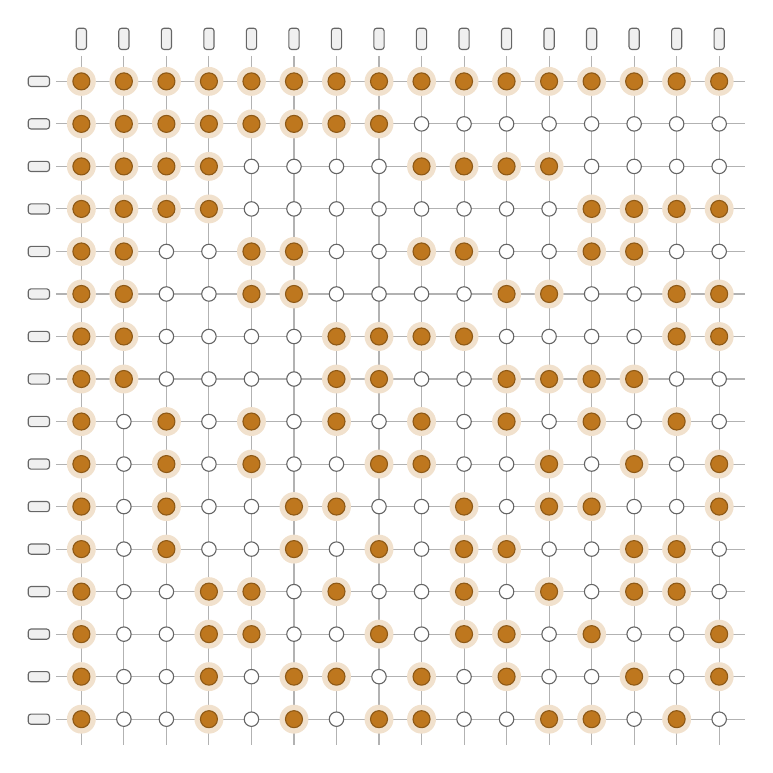
\begin{tikzpicture}[x=5.4mm,y=5.4mm]
  \foreach \i in {0,...,15}{
    \draw[black!30] (-.6,-\i)--(15.6,-\i);
    \draw[black!30] (\i,.6)--(\i,-15.6);
    \draw[rounded corners=1pt,fill=black!6,draw=black!60] (-1.25,-\i-.12) rectangle (-.75,-\i+.12);
    \draw[rounded corners=1pt,fill=black!6,draw=black!60] (\i-.12,.75) rectangle (\i+.12,1.25);
  }
  \foreach \row [count=\i from 0] in {{1,1,1,1,1,1,1,1,1,1,1,1,1,1,1,1},{1,1,1,1,1,1,1,1,0,0,0,0,0,0,0,0},{1,1,1,1,0,0,0,0,1,1,1,1,0,0,0,0},{1,1,1,1,0,0,0,0,0,0,0,0,1,1,1,1},{1,1,0,0,1,1,0,0,1,1,0,0,1,1,0,0},{1,1,0,0,1,1,0,0,0,0,1,1,0,0,1,1},{1,1,0,0,0,0,1,1,1,1,0,0,0,0,1,1},{1,1,0,0,0,0,1,1,0,0,1,1,1,1,0,0},{1,0,1,0,1,0,1,0,1,0,1,0,1,0,1,0},{1,0,1,0,1,0,0,1,1,0,0,1,0,1,0,1},{1,0,1,0,0,1,1,0,0,1,0,1,1,0,0,1},{1,0,1,0,0,1,0,1,0,1,1,0,0,1,1,0},{1,0,0,1,1,0,1,0,0,1,0,1,0,1,1,0},{1,0,0,1,1,0,0,1,0,1,1,0,1,0,0,1},{1,0,0,1,0,1,1,0,1,0,1,0,0,1,0,1},{1,0,0,1,0,1,0,1,1,0,0,1,1,0,1,0}}{
    \foreach \lamp [count=\j from 0] in \row{
      \ifnum\lamp=1
        \fill[glowgold!22] (\j,-\i) circle[radius=.34];
        \filldraw[draw=glowgold!75!black,fill=glowgold] (\j,-\i) circle[radius=.2];
      \else
        \draw[draw=black!60,fill=white] (\j,-\i) circle[radius=.17];
      \fi
    }
  }
\end{tikzpicture}
\caption{The board of $\mathrm{had}_{16.3}$, with 136 lit lamps. With the row and column switches, the best that one can do is 156 lit lamps, and this can be done in 43008 ways, leading to 21504 distinct boards.}\label{fig:board}
\end{figure}

With $H_{jk}=\pm1$ recording the lamps and $a_j,b_k=\pm1$ the switches, the number of lit lamps minus the number of dark ones is
\[
 \Omega=\sum_{jk}H_{jk}a_jb_k=\langle Hb,a\rangle
\]
and the real glow of $H$ is the law of $\Omega$, for random switches \cite{bhm,ba1}. In physical terms, $\Omega$ is, up to a factor, minus the energy of a system of Ising spins. Take 2 layers of $N$ parallel wires, the wires of one layer crossing those of the other at right angles, put an Ising spin on each wire, $a_j$ on the $j$th row wire and $b_k$ on the $k$th column wire, and couple the 2 spins at each crossing:
\[
 E(a,b)=-\frac{1}{\sqrt N}\sum_{jk}H_{jk}a_jb_k=-\frac{\Omega}{\sqrt N}
\]
The game of Gale and Berlekamp is then the search for the ground states, and the real glow is the density of states, normalized to be a probability. When $H$ is Hadamard the coupling matrix $H/\sqrt N$ is orthogonal, and the coupling matrix of all the $2N$ spins is symmetric and orthogonal, with eigenvalues $\pm1$. This is the situation of the random orthogonal model of Marinari, Parisi and Ritort \cite{mp1,mp2}, which was introduced as a disordered version of their deterministic sine and cosine models, and which has a glass transition \cite{cdl,mp2,ppo}. Their fully frustrated hypercube \cite{mp3} is also of this type, and is in fact an Ising array too, for a weighing matrix. The complex version of the array is the one of Chandra, Ioffe and Sherrington \cite{cis}, studied in \cite{cot}, and as explained there, all this is one more beginning of an answer to the old question of Jones on the statistical mechanical meaning of the Hadamard matrices \cite{jo2}.

Our first result is about the 5 arrays of order 16. Let $n_H(\omega)$ be the number of pairs $(a,b)$ with $\Omega=\omega$, and let $r$ be the 2-rank of the core of $H$, that is, of the binary matrix $M$ given by $H_{jk}=(-1)^{M_{jk}}$, after making the first row and column of $H$ positive and removing them.

\begin{samepage}
\begin{introthm}\label{intro:spectrum}
The densities of states of the $5$ Ising arrays of order $16$ form a $1$-parameter family. With $n$ being the density of states of $\mathrm{had}_{16.3}$, we have
\[
 n_H(64-8k)=n(64-8k)+(-1)^k\binom{16}{k}c_H
\]
for $k=0,\ldots,16$, and $n_H(\omega)=n(\omega)$ for $\omega=4(8)$, where $c_H=2^{14-r}-128$ is the number of crystalline ground states, which are $896,384,128,0,0$ for the classes $\mathrm{had}_{16.0},\ldots,\mathrm{had}_{16.4}$.
\end{introthm}
\end{samepage}

Equivalently, the partition functions are related by $Z_H(\beta)=Z(\beta)+c_H(2\sinh\beta)^{16}$. The numbers $384,128$, and the absence of crystalline states for $\mathrm{had}_{16.3},\mathrm{had}_{16.4}$, appear in \cite{scg}, in the language of bent sequences. This contains the 2-adic description of these densities of states, obtained by reduction modulo 16, and we show in fact that for any $N$ the law of $\Omega$ modulo 16 is determined by $N$ and $r$. At $N=20$ the 3 densities of states coincide, so that the 3 inequivalent arrays of order 20 have exactly the same thermodynamics, at $N=24$ the 60 densities of states form a 2-parameter family, given by the number of ground states and by the 4-profile below, and at $N=28$ the 487 densities of states form a 4-parameter family.

Behind Theorem~\ref{intro:spectrum} there is a general fact, the universality of the moments of $\Omega$, which holds up to order 14, and which is broken at order 16 by the 4-profile of $H$, studied by Cooper, Milas and Wallis \cite{cmw}:

\begin{samepage}
\begin{introthm}\label{intro:moments}
For a real Hadamard matrix of order $N$ and $p\leq7$, the moment $E(\Omega^{2p})$ is a polynomial in $N$, which does not depend on $H$. The first cumulants are
\[
 \kappa_2=N^2,\quad\kappa_4=-6N^3+4N^2,\quad\kappa_6=240N^4-480N^3+256N^2
\]
and at order $16$ we have $E(\Omega^{16})=U(N)+\frac{2^8\,16!}{4!}\,P_4(H)$, with $U$ a polynomial, and with
\[
 P_4(H)=\sum_{|I|=4}\Big(\sum_k\prod_{j\in I}H_{jk}\Big)^4
\]
the sum being over the sets of $4$ rows.
\end{introthm}
\end{samepage}

The leading terms of the cumulants are universal at every order, and are those of a Haar orthogonal matrix. This gives the free energy at high temperature, as for the complex arrays in \cite{cot}, and the result agrees with the replica-symmetric free energy of the random orthogonal model computed in \cite{mp2}:

\begin{samepage}
\begin{introthm}\label{intro:free}
For a real Hadamard matrix of order $N$, the cumulants are
\[
 \kappa_{2k}=(-1)^{k-1}(2k-1)!\,Cat_{k-1}N^{k+1}+O(N^k)
\]
with $Cat_j=\binom{2j}{j}/(j+1)$, uniformly in $H$. Thus, coefficientwise in $\beta$, we have
\[
 \frac{1}{N}\log E\left(e^{\beta\Omega/\sqrt N}\right)\to\frac{1}{2}\left(\sqrt{1+4\beta^2}-1-\log\frac{1+\sqrt{1+4\beta^2}}{2}\right)
\]
and the entropy per row wire of this continued paramagnetic solution, $2\log2-\frac{1}{2}\log\frac{1+\sqrt{1+4\beta^2}}{2}$, vanishes at $\beta=\sqrt{240}$.
\end{introthm}
\end{samepage}

The vanishing of this entropy signals that the paramagnetic solution must break down before, presumably at a glass transition, as in the random energy model \cite{der}, and in the normalization of \cite{mp2} it happens at temperature $4/\sqrt{240}\simeq0.258$, just below the replica symmetry breaking temperature $T_{RSB}\simeq0.26$ found there for the random orthogonal model. At low temperature, the regular Hadamard matrices, whose row and column sums are all equal, provide crystalline states of energy exactly $-N$, the analogs of the crystalline states found in \cite{mp2} for the sine model when $2N+1$ is prime, and $\mathrm{had}_{16.3}$ has no such state. The number of its ground states can be read from \cite{gbt}, in the language of Bell inequalities, and what is new here is their structure:

\begin{samepage}
\begin{introthm}\label{intro:ground}
The ground states of the Ising array of $\mathrm{had}_{16.3}$ have energy $-14$, instead of $-16$ for the regular matrices, and they are $43008$ in number. They form $3$ orbits of size $14336$ under the symmetry group of the matrix, which has order $86016$, and in $2$ of these orbits $3$ of the row spins feel no field, and are free, while in $2$ of them the same happens for $3$ of the column spins.
\end{introthm}
\end{samepage}

The number of crystalline states also controls the crystallization temperature, obtained by equating the free energy of the crystal with the paramagnetic free energy of Theorem~\ref{intro:free}, and this predicts the maxima of the specific heat at $N=16$. For the Walsh matrices the crystalline states are the bent functions, whose number is a well-known open problem. In the last section we simulate the dynamics, finding a crystallization for $W_{64},W_{256}$, while for $W_{1024},W_{4096}$ the crystal is missed, as for the sine model, the cooling of $W_{4096}$ ending at about the same energy as for the Paley matrices of order 252 and 1020. We also compute the exact densities of states at $N=24,28$, which form families with 2 and 4 parameters, the ground states being invisible in the moments up to order 22, and which at $N=28$ determine the matrix up to equivalence and transposition, at $N=32$, for 360 matrices, whose densities of states are distinct, and lie in an affine space of dimension 8, and at $N=36$, for 9 regular matrices, where the crystallization temperature predicts the maxima of the specific heat within $0.0025$.

The paper is organized as follows. Section~\ref{sec:ising} recalls the Ising model and its versions, Section~\ref{sec:model} explains our model, Section~\ref{sec:2adic} discusses its energy levels modulo powers of 2, Section~\ref{sec:moments} contains the universality of the moments, Section~\ref{sec:free} the free energy at high temperature, Section~\ref{sec:ground} the ground states, Section~\ref{sec:exact} the exact thermodynamics at $N=16,20$, where Theorem~\ref{intro:spectrum} is proved, and Section~\ref{sec:larger} the dynamics, and the densities of states at $N=24,28,32,36$.

\medskip

{\em Acknowledgements.} We would like to thank Gemini and Grok for useful discussions. We are grateful as well to $\mathrm{had}_{16.3}$: as long as this matrix produces interesting physics, we will not put it in bistochastic form, and we are not in a hurry with our project \cite{com}.

\section{The Ising model and its versions}\label{sec:ising}

We first recall the Ising model, and some of its versions, which lead to the arrays studied in this paper. This section is intended for the readers coming from operator algebras, quantum algebra or combinatorics, and can be skipped by the physicists. For more on all this we refer to the books \cite{bax,mpv}, and for the history to Brush \cite{bru}.

\medskip

\noindent\textbf{The original model.} The Ising model was proposed by Lenz \cite{len}, and studied by his student Ising \cite{isi}, as a model of ferromagnetism. A spin $\sigma_x\in\{\pm1\}$ sits at each vertex $x$ of a graph $\Gamma$, typically the lattice $\mathbb Z^d$, or a finite piece of it, and neighboring spins interact, with energy
\[
 E(\sigma)=-J\sum_{x\sim y}\sigma_x\sigma_y
\]
where $J>0$, the sum being over the edges of $\Gamma$. Aligned neighbors lower the energy, so the ground states are the 2 constant configurations. At temperature $T$, with inverse temperature $\beta=1/T$, the configurations are distributed according to the Gibbs measure $P(\sigma)=e^{-\beta E(\sigma)}/Z$, where $Z=\sum_\sigma e^{-\beta E(\sigma)}$ is the partition function. The free energy per spin is $-\frac{1}{\beta}\lim\frac{1}{|\Gamma|}\log Z$, the limit being over finite pieces of the lattice whose size goes to infinity, and a phase transition is a temperature at which this function is not analytic. At high temperature the spins are disordered, and at low temperature they may align, producing a spontaneous magnetization, as in Figure~\ref{fig:lattice}.

\begin{figure}[htb!]
\centering
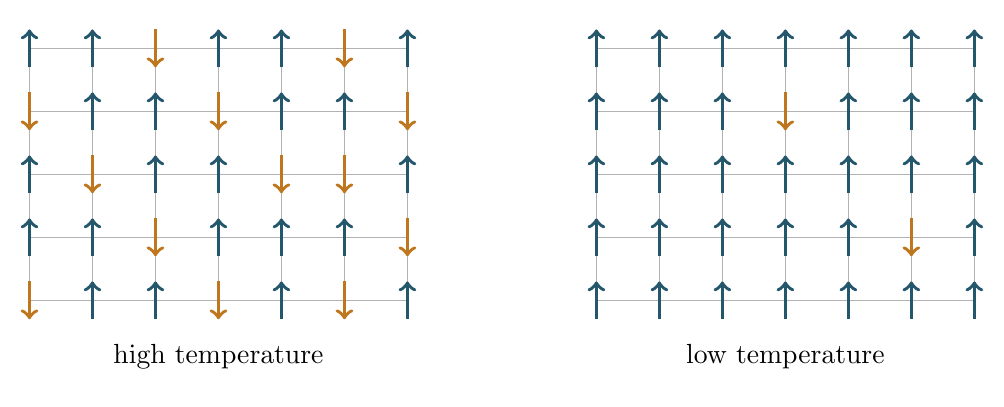
\begin{tikzpicture}[x=8mm,y=8mm]
  \foreach \row [count=\i from 0] in {{1,1,-1,1,1,-1,1},{-1,1,1,-1,1,1,-1},{1,-1,1,1,-1,-1,1},{1,1,-1,1,1,1,-1},{-1,1,1,-1,1,-1,1}}{
    \foreach \s [count=\j from 0] in \row{
      \ifnum\j<6 \draw[black!30] (\j,-\i)--(\j+1,-\i); \fi
      \ifnum\i<4 \draw[black!30] (\j,-\i)--(\j,-\i-1); \fi
      \ifnum\s=1 \draw[->,glowblue,line width=1.3pt] (\j,-\i-.3)--(\j,-\i+.3);
      \else \draw[->,glowgold,line width=1.3pt] (\j,-\i+.3)--(\j,-\i-.3); \fi
    }}
  \begin{scope}[shift={(9,0)}]
  \foreach \row [count=\i from 0] in {{1,1,1,1,1,1,1},{1,1,1,-1,1,1,1},{1,1,1,1,1,1,1},{1,1,1,1,1,-1,1},{1,1,1,1,1,1,1}}{
    \foreach \s [count=\j from 0] in \row{
      \ifnum\j<6 \draw[black!30] (\j,-\i)--(\j+1,-\i); \fi
      \ifnum\i<4 \draw[black!30] (\j,-\i)--(\j,-\i-1); \fi
      \ifnum\s=1 \draw[->,glowblue,line width=1.3pt] (\j,-\i-.3)--(\j,-\i+.3);
      \else \draw[->,glowgold,line width=1.3pt] (\j,-\i+.3)--(\j,-\i-.3); \fi
    }}
  \end{scope}
  \node at (3,-4.9) {high temperature};
  \node at (12,-4.9) {low temperature};
\end{tikzpicture}
\caption{The Ising model on a piece of the square lattice, with typical configurations at high temperature, where the spins are disordered, and at low temperature, where most of them are aligned.}\label{fig:lattice}
\end{figure}

In dimension 1 there is no phase transition, as found by Ising, and his computation is a nice exercise in linear algebra:

\begin{samepage}
\begin{prop}\label{prop:ising1}
For a ring of $n$ spins, with energy $E(\sigma)=-J\sum_x\sigma_x\sigma_{x+1}$, indices modulo $n$, we have
\[
 Z=(2\cosh\beta J)^n+(2\sinh\beta J)^n
\]
so that $\frac{1}{n}\log Z\to\log(2\cosh\beta J)$, which is analytic in $\beta$. Thus there is no phase transition.
\end{prop}
\end{samepage}

\begin{proof}
Consider the transfer matrix
\[
 T=(e^{\beta Jst})_{s,t=\pm1}=\begin{pmatrix}e^{\beta J}&e^{-\beta J}\\e^{-\beta J}&e^{\beta J}\end{pmatrix}
\]
We have then $Z=\sum_\sigma\prod_xT_{\sigma_x\sigma_{x+1}}=Tr(T^n)$, and the eigenvalues of $T$ are $e^{\beta J}\pm e^{-\beta J}$.
\end{proof}

Ising concluded that there should be no transition in higher dimensions either, which turned out to be wrong. In dimension 2, Onsager computed the free energy of the square lattice exactly \cite{ons}, by using a transfer matrix of size $2^n$ for a strip of width $n$, and found a transition at $\sinh(2\beta J)=1$, that is, $\beta J=\log(1+\sqrt2)/2\simeq0.4407$. This was the start of the theory of exactly solved models \cite{bax}.

\medskip

\noindent\textbf{Mean field.} The simplest version where a transition can be seen is the Curie--Weiss model, going back to the molecular field of Weiss \cite{wei}, where all the pairs of spins interact, with strength $J/n$. With $M=\sum_x\sigma_x$ the magnetization, the energy is
\[
 E(\sigma)=-\frac{J}{n}\sum_{x<y}\sigma_x\sigma_y=-\frac{J}{2n}(M^2-n)
\]
so it only depends on $M$, and the partition function is a sum of $n+1$ terms, involving binomial coefficients. With $I(m)=\frac{1+m}{2}\log(1+m)+\frac{1-m}{2}\log(1-m)$, Stirling's formula gives:

\begin{samepage}
\begin{prop}\label{prop:cw}
For the Curie--Weiss model we have
\[
 \frac{1}{n}\log Z\to\log2+\max_{m\in[-1,1]}\left(\frac{\beta Jm^2}{2}-I(m)\right)
\]
and the maximum is attained at solutions of $m=\tanh(\beta Jm)$. For $\beta J\leq1$ the only solution is $m=0$, and for $\beta J>1$ there are $3$ solutions, $0$ and $\pm m_*$, the maximum being attained at $\pm m_*$, giving a phase transition at $\beta J=1$, with spontaneous magnetization $m_*$ below it.
\end{prop}
\end{samepage}

\begin{proof}
The term with $M=nm$ is $\binom{n}{n(1+m)/2}e^{\beta J(nm^2-1)/2}=e^{n(\log2-I(m)+\beta Jm^2/2)+o(n)}$, and since there are $n+1$ terms, the largest one gives the limit. The critical points satisfy $\beta Jm=I'(m)=artanh(m)$, and since $\tanh$ is concave on $[0,\infty)$, with slope 1 at 0, the equation $m=\tanh(\beta Jm)$ has a solution $m>0$ precisely when $\beta J>1$, this solution being then the maximum.
\end{proof}

In our arrays all the spins of one layer interact with all the spins of the other layer, so these are mean field models too. However, the couplings $H_{jk}/\sqrt N$ have both signs, and strength $1/\sqrt N$ instead of $1/n$, and this changes everything.

\medskip

\noindent\textbf{Disorder and frustration.} Spin glasses were introduced by Edwards and Anderson \cite{ean}, as Ising models on the lattice with random couplings $J_{xy}$, of both signs, and with energy $-\sum_{x\sim y}J_{xy}\sigma_x\sigma_y$. Their mean field version is the model of Sherrington and Kirkpatrick \cite{ski}, where all the pairs interact, with independent Gaussian couplings of variance $1/n$. This model has a glass transition at $\beta=1$, and its free energy was found by Parisi \cite{par}, with his replica symmetry breaking, a formula proved by Talagrand \cite{tal}. The key notion here is frustration, due to Toulouse \cite{tou}: a cycle of the graph is frustrated when the product of the couplings around it is negative, because then no configuration can satisfy all the couplings, in the sense of having $J_{xy}\sigma_x\sigma_y>0$ on all its edges, as in Figure~\ref{fig:frustsquare}.

\begin{figure}[htb!]
\centering
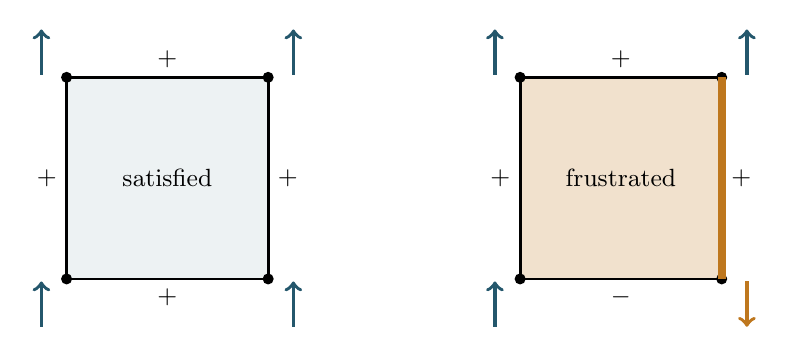
\begin{tikzpicture}[x=16mm,y=16mm,font=\small]
  \foreach \shift/\fr in {0/0,3.6/1}{
    \begin{scope}[shift={(\shift,0)}]
      \ifnum\fr=1 \fill[glowgold!22] (0,0) rectangle (1.6,1.6); \else \fill[glowblue!8] (0,0) rectangle (1.6,1.6); \fi
      \draw[line width=1pt] (0,0) rectangle (1.6,1.6);
      \node[above] at (.8,1.6) {$+$}; \node[left] at (0,.8) {$+$}; \node[right] at (1.6,.8) {$+$};
      \ifnum\fr=1 \node[below] at (.8,0) {$-$}; \node at (.8,.8) {frustrated}; \else \node[below] at (.8,0) {$+$}; \node at (.8,.8) {satisfied}; \fi
      \foreach \x/\y in {0/0,1.6/0,0/1.6,1.6/1.6} \fill (\x,\y) circle[radius=2pt];
      \foreach \x/\y in {-.2/1.8,1.8/1.8,-.2/-.2} \draw[->,glowblue,line width=1.3pt] (\x,\y-.18)--(\x,\y+.18);
      \ifnum\fr=1 \draw[glowgold,line width=3pt] (1.6,0)--(1.6,1.6); \draw[->,glowgold,line width=1.3pt] (1.8,-.02)--(1.8,-.38);
      \else \draw[->,glowblue,line width=1.3pt] (1.8,-.38)--(1.8,-.02); \fi
    \end{scope}}
\end{tikzpicture}
\caption{A square of the lattice, with the signs of the couplings on its edges. On the left all the couplings are satisfied by aligned spins, while on the right, whatever the spins are, at least one coupling is violated, here the one drawn thick.}\label{fig:frustsquare}
\end{figure}

What matters here is the product of the signs around the cycle, and not their number. A square with 2 negative couplings is not frustrated, the spins simply changing sign across them, while a square with 3 negative couplings is frustrated, as in Figure~\ref{fig:frustmore}.

\begin{figure}[htb!]
\centering
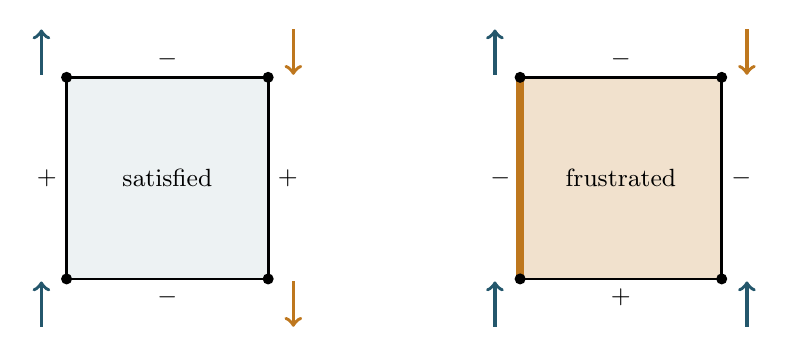
\begin{tikzpicture}[x=16mm,y=16mm,font=\small]
  \fill[glowblue!8] (0,0) rectangle (1.6,1.6);
  \draw[line width=1pt] (0,0) rectangle (1.6,1.6);
  \node[above] at (.8,1.6) {$-$}; \node[below] at (.8,0) {$-$}; \node[left] at (0,.8) {$+$}; \node[right] at (1.6,.8) {$+$};
  \node at (.8,.8) {satisfied};
  \foreach \x/\y in {0/0,1.6/0,0/1.6,1.6/1.6} \fill (\x,\y) circle[radius=2pt];
  \foreach \x/\y in {-.2/1.8,-.2/-.2} \draw[->,glowblue,line width=1.3pt] (\x,\y-.18)--(\x,\y+.18);
  \foreach \x/\y in {1.8/1.8,1.8/-.2} \draw[->,glowgold,line width=1.3pt] (\x,\y+.18)--(\x,\y-.18);
  \begin{scope}[shift={(3.6,0)}]
    \fill[glowgold!22] (0,0) rectangle (1.6,1.6);
    \draw[line width=1pt] (0,0) rectangle (1.6,1.6);
    \draw[glowgold,line width=3pt] (0,0)--(0,1.6);
    \node[above] at (.8,1.6) {$-$}; \node[left] at (0,.8) {$-$}; \node[right] at (1.6,.8) {$-$}; \node[below] at (.8,0) {$+$};
    \node at (.8,.8) {frustrated};
    \foreach \x/\y in {0/0,1.6/0,0/1.6,1.6/1.6} \fill (\x,\y) circle[radius=2pt];
    \foreach \x/\y in {-.2/1.8,1.8/-.2,-.2/-.2} \draw[->,glowblue,line width=1.3pt] (\x,\y-.18)--(\x,\y+.18);
    \draw[->,glowgold,line width=1.3pt] (1.8,1.98)--(1.8,1.62);
  \end{scope}
\end{tikzpicture}
\caption{A square with 2 negative couplings, which is not frustrated, the product of its signs being positive, and a square with 3 negative couplings, which is frustrated: whatever the spins are, at least one coupling is violated, here the one drawn thick.}\label{fig:frustmore}
\end{figure}

On lattices which are not bipartite, such as the triangular lattice of Wannier \cite{wan}, even the antiferromagnet, with all its couplings negative, is frustrated, its triangles having 3 negative couplings. On bipartite graphs this cannot happen, because flipping the spins on one side turns the antiferromagnet into the ferromagnet. This applies to our arrays, which live on the complete bipartite graph $K_{N,N}$, so all their frustration comes from the signs of the couplings.

The energy is invariant under the gauge transformations $\sigma_x\to\varepsilon_x\sigma_x$, $J_{xy}\to\varepsilon_x\varepsilon_yJ_{xy}$, with $\varepsilon_x=\pm1$, and the frustration of the cycles is gauge invariant. Mattis observed that the couplings $J_{xy}=J\xi_x\xi_y$, with $\xi_x$ random signs, look disordered, but are gauge equivalent to the ferromagnet \cite{mat}. In general:

\begin{samepage}
\begin{prop}\label{prop:mattis}
Couplings $J_{xy}\in\{\pm J\}$ on a connected graph are gauge equivalent to the ferromagnet, $J_{xy}=J$, precisely when no cycle is frustrated.
\end{prop}
\end{samepage}

\begin{proof}
If $J_{xy}=J\varepsilon_x\varepsilon_y$, the product around any cycle is a positive power of $J$, times squares. Conversely, choose a spanning tree, put $\varepsilon=1$ at its root, and define $\varepsilon$ along the tree by $\varepsilon_y=\varepsilon_x\,sgn(J_{xy})$. Any other edge closes a cycle with the tree, which is not frustrated, so $J_{xy}=J\varepsilon_x\varepsilon_y$ on this edge too.
\end{proof}

For our arrays the graph is the complete bipartite graph between the 2 layers, and the case of a Mattis ferromagnet is that of a matrix $H=ab^t$ of rank 1. The Hadamard matrices are at the opposite end, being maximally frustrated, in a sense that will be made precise in Section~\ref{sec:model}.

\medskip

\noindent\textbf{Orthogonal couplings.} Marinari, Parisi and Ritort found that disorder is not needed for glassy behavior \cite{mp1,mp2}. They studied deterministic models, coming from the problem of the binary sequences with low autocorrelation, and in particular the sine model, whose couplings are essentially the imaginary parts of a Fourier matrix, and which form an orthogonal matrix. They also introduced its disordered counterpart, the random orthogonal model, whose couplings form a random symmetric orthogonal matrix, and they found the same thermodynamics at high temperature, and the same glass transition. The mean field equations of these models were derived by Parisi and Potters \cite{ppo}, and the role of the spectrum of the couplings was studied by Cherrier, Dean and Lef\`evre \cite{cdl}. For special sizes the sine model also has crystalline ground states, of very low energy, which are not reached by cooling, the system getting stuck in the glass. The same glass transition was found for the fully frustrated hypercube \cite{mp3}, whose couplings are signs on the edges of a hypercube, with all the square faces frustrated, and the glassy phase of these models shows aging, as in the matrix models of Cugliandolo, Kurchan, Parisi and Ritort \cite{ckp}, while the hypercube with planar rotators has no transition at all \cite{mp3}. The Hadamard matrices themselves appear in this context as crystals, being the ground states of the $\pm1$ matrix model in \cite{ckp}, and of the hard matrix model of \cite{del}, which fails to find them upon cooling, and shows all the features of a glass. Our arrays are models of this type, the Hadamard condition making the couplings orthogonal, as summarized in Figure~\ref{fig:tree}.

\begin{figure}[htb!]
\centering
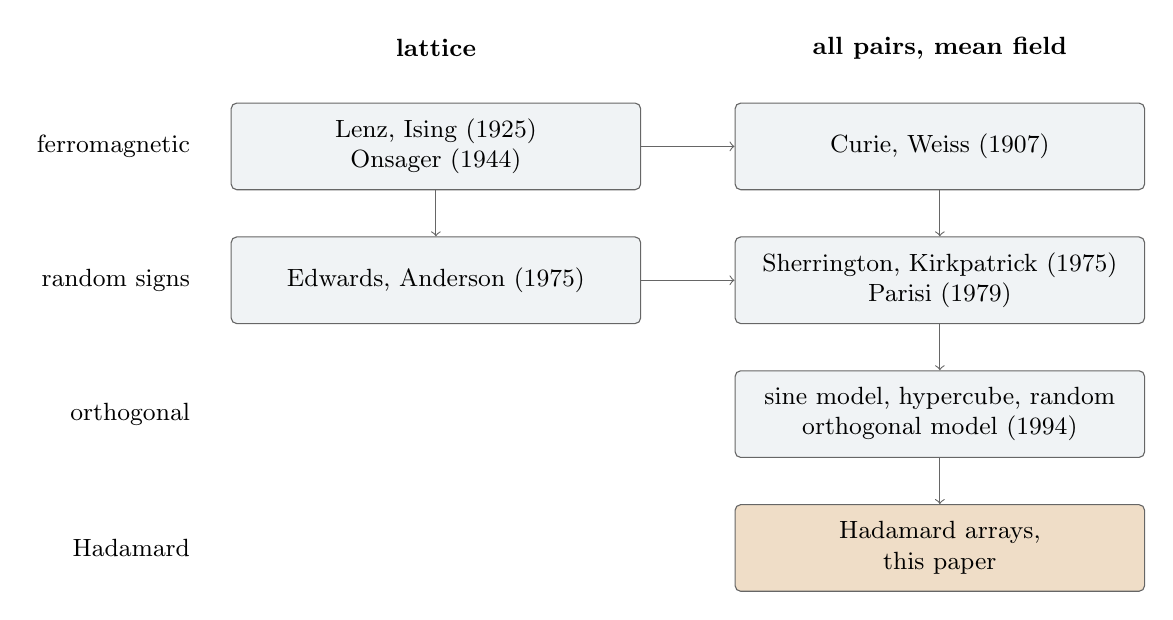
\begin{tikzpicture}[font=\small,box/.style={draw=black!60,rounded corners=2pt,align=center,minimum width=52mm,minimum height=11mm,fill=glowblue!7}]
  \node at (0,1.25) {\textbf{lattice}}; \node at (6.4,1.25) {\textbf{all pairs, mean field}};
  \node[left,align=right] at (-3,0) {ferromagnetic}; \node[left,align=right] at (-3,-1.7) {random signs};
  \node[left,align=right] at (-3,-3.4) {orthogonal}; \node[left,align=right] at (-3,-5.1) {Hadamard};
  \node[box] (a) at (0,0) {Lenz, Ising (1925)\\Onsager (1944)};
  \node[box] (b) at (6.4,0) {Curie, Weiss (1907)};
  \node[box] (c) at (0,-1.7) {Edwards, Anderson (1975)};
  \node[box] (d) at (6.4,-1.7) {Sherrington, Kirkpatrick (1975)\\Parisi (1979)};
  \node[box] (e) at (6.4,-3.4) {sine model, hypercube, random\\orthogonal model (1994)};
  \node[box,fill=glowgold!25] (f) at (6.4,-5.1) {Hadamard arrays,\\this paper};
  \draw[->,black!60] (a)--(b); \draw[->,black!60] (c)--(d);
  \draw[->,black!60] (a)--(c); \draw[->,black!60] (b)--(d); \draw[->,black!60] (d)--(e); \draw[->,black!60] (e)--(f);
\end{tikzpicture}
\caption{Some versions of the Ising model. The arrows go from the lattice to the mean field models, from the ferromagnets to the spin glasses, from the random couplings to the deterministic orthogonal ones, and finally to the Hadamard couplings.}\label{fig:tree}
\end{figure}

Note that the sine model and the random orthogonal model are mean field models too, all the pairs of spins interacting. Many further versions are possible. For our arrays, a natural one is to add couplings inside the layers, for instance Ising chains along each layer, with correlation $\tanh(K)^{|j-l|}$ between the wires $j,l$, as done in \cite{cot} with Villain chains for the complex arrays. This would interpolate between the density of states and the fully aligned limit, where $\Omega$ becomes the sum of the entries of $H$, and it would be interesting to study this crossover.

\medskip

\noindent\textbf{High temperature.} The basic tool at high temperature is the expansion of van der Waerden \cite{vdw}. Since $\sigma_x\sigma_y=\pm1$, we have $e^{\beta J_{xy}\sigma_x\sigma_y}=\cosh(\beta J_{xy})(1+\sigma_x\sigma_y\tanh(\beta J_{xy}))$, and expanding the product over the edges gives a sum over the subsets of edges, as in Figure~\ref{fig:loops}. At high temperature the numbers $\tanh(\beta J_{xy})$ are small, and the partition function is governed by the short loops, the frustrated loops having negative weights. In Section~\ref{sec:moments} we will use the same idea for the moments of the density of states, which will be sums over bipartite multigraphs, reducing to graphs with all degrees even, the smallest graph which feels the Hadamard matrix, beyond its orthogonality, being the complete bipartite graph $K_{4,4}$.

\begin{figure}[htb!]
\centering
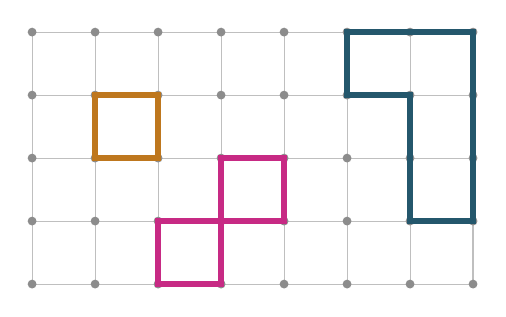
\begin{tikzpicture}[x=8mm,y=8mm]
  \foreach \i in {0,...,4}\foreach \j in {0,...,7}{
    \ifnum\j<7 \draw[black!25] (\j,-\i)--(\j+1,-\i); \fi
    \ifnum\i<4 \draw[black!25] (\j,-\i)--(\j,-\i-1); \fi
    \fill[black!45] (\j,-\i) circle[radius=1.6pt];}
  \draw[glowgold,line width=2pt] (1,-1) rectangle (2,-2);
  \draw[glowblue,line width=2pt] (5,0)--(7,0)--(7,-3)--(6,-3)--(6,-1)--(5,-1)--cycle;
  \draw[magenta!80!black,line width=2pt] (2,-3) rectangle (3,-4);
  \draw[magenta!80!black,line width=2pt] (3,-2) rectangle (4,-3);
\end{tikzpicture}
\caption{An even subgraph of the square lattice, where each vertex has even degree, here 0, 2 or 4. Such subgraphs are edge-disjoint unions of cycles, and they are the terms of the high-temperature expansion.}\label{fig:loops}
\end{figure}

In formulas, the expansion is as follows, and this is the basic structure behind all the high-temperature expansions in statistical mechanics:

\begin{samepage}
\begin{thm}\label{thm:vdw}
For a finite graph $\Gamma$, with vertex set $V$, edge set $E$, and couplings $J_e$ on its edges, the partition function of the Ising model with energy $-\sum_{xy\in E}J_{xy}\sigma_x\sigma_y$ is
\[
 Z=2^{|V|}\prod_{e\in E}\cosh(\beta J_e)\sum_F\prod_{e\in F}\tanh(\beta J_e)
\]
the sum being over the subsets $F\subset E$ such that each vertex has even degree in $F$.
\end{thm}
\end{samepage}

\begin{proof}
By expanding the product $\prod_{xy\in E}(1+\sigma_x\sigma_y\tanh(\beta J_{xy}))$, the partition function is $\prod_e\cosh(\beta J_e)$ times the sum over $F\subset E$ of $\prod_{e\in F}\tanh(\beta J_e)\sum_\sigma\prod_x\sigma_x^{d_F(x)}$, with $d_F(x)$ being the degree of $x$ in $F$. The sum over $\sigma$ is $2^{|V|}$ if all the degrees $d_F(x)$ are even, and $0$ otherwise.
\end{proof}

\section{Ising spins on crossed wires}\label{sec:model}

We now explain our model, and its relation with the switching game, with frustration, and with the orthogonal couplings.

\medskip

\noindent\textbf{The array.}
Let $H\in M_N(\pm1)$. The Ising array of $H$ consists of 2 layers of $N$ parallel wires, crossing at right angles, with an Ising spin on each wire, $a_j\in\{\pm1\}$ on the $j$th row wire and $b_k\in\{\pm1\}$ on the $k$th column wire, and with the 2 spins at the crossing $jk$ coupled with strength $H_{jk}/\sqrt N$, as in Figure~\ref{fig:array}. The energy is
\[
 E(a,b)=-\frac{1}{\sqrt N}\sum_{jk}H_{jk}a_jb_k
\]
and at inverse temperature $\beta$ the partition function is
\[
 Z_H(\beta)=\sum_{a,b}e^{-\beta E(a,b)}=4^NE\left(e^{\beta\Omega/\sqrt N}\right)
\]
with $\Omega=\langle Hb,a\rangle$ and with $a,b$ uniform. The normalization $1/\sqrt N$ is the one which makes the free energy extensive, and when $H$ is Hadamard it makes the coupling matrix orthogonal.

\begin{figure}[htb!]
\centering
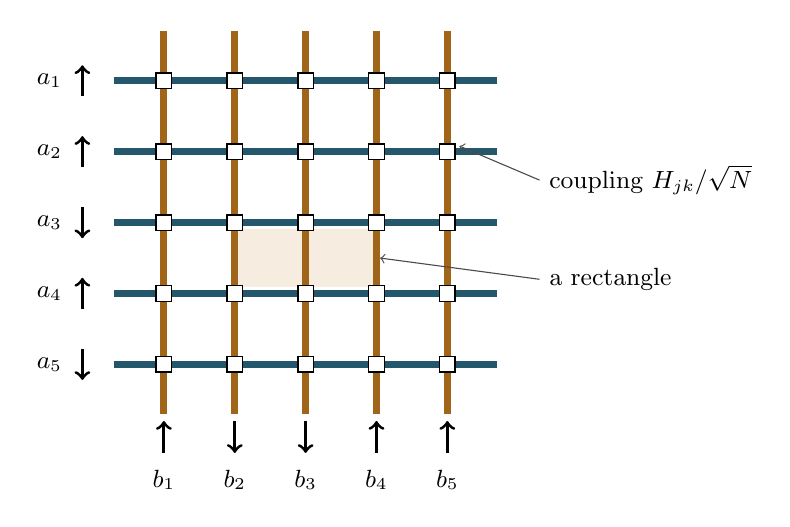
\begin{tikzpicture}[x=9mm,y=9mm,font=\small]
  \fill[glowgold!14] (1,1) rectangle (3,2);
  \foreach \k/\lab/\s in {0/1/1,1/2/-1,2/3/-1,3/4/1,4/5/1}{
    \draw[glowgold!85!black,line width=2.6pt] (\k,-.7)--(\k,4.7);
    \node[below] at (\k,-1.35) {$b_\lab$};
    \ifnum\s=1 \draw[->,line width=1.1pt,black] (\k,-1.25)--(\k,-.8);
    \else \draw[->,line width=1.1pt,black] (\k,-.8)--(\k,-1.25); \fi
  }
  \foreach \j/\lab/\s in {0/1/1,1/2/1,2/3/-1,3/4/1,4/5/-1}{
    \draw[white,line width=4.6pt] (-.7,4-\j)--(4.7,4-\j);
    \draw[glowblue,line width=2.6pt] (-.7,4-\j)--(4.7,4-\j);
    \node[left] at (-1.3,4-\j) {$a_\lab$};
    \ifnum\s=1 \draw[->,line width=1.1pt,black] (-1.15,4-\j-.22)--(-1.15,4-\j+.22);
    \else \draw[->,line width=1.1pt,black] (-1.15,4-\j+.22)--(-1.15,4-\j-.22); \fi
  }
  \foreach \j in {0,...,4}\foreach \k in {0,...,4}
    \filldraw[draw=black,fill=white,line width=.5pt] (\k-.11,\j-.11) rectangle (\k+.11,\j+.11);
  \draw[->,black!70] (5.3,2.6) node[right,text=black] {coupling $H_{jk}/\sqrt N$} -- (4.17,3.08);
  \draw[->,black!70] (5.3,1.2) node[right,text=black] {a rectangle} -- (3.05,1.5);
\end{tikzpicture}
\caption{The Ising array with $N=5$. The row wires carry the spins $a_j$, the column wires the spins $b_k$, and the 2 spins at each crossing are coupled. The shaded rectangle has corners at 4 crossings, and is frustrated when the product of the 4 couplings is negative.}\label{fig:array}
\end{figure}

In the language of the switching game, $H$ is the board, the spins are the switches, and $\Omega$ is the number of lit lamps minus the number of dark ones, so that the lowest energy is the best score. Berlekamp built such a board with 100 lamps for the common room at Bell Labs, and the game on that board was solved by Fishburn and Sloane \cite{fsl}. In coding terms, the boards reachable from the all-dark one form a binary linear code, and the best score is related to the covering radius of that code \cite{slo}, whose computation is hard \cite{rvi}, with good approximation schemes being available \cite{kas}.

\medskip

\noindent\textbf{Gauge and frustration.}
Reversing the spin of the $j$th row wire, while changing the sign of the $j$th row of $H$, does not change the energy, and the same holds for the columns. Thus the physics of the array depends only on the equivalence class of $H$ under sign changes of its rows and columns, and since the spins of a layer are all coupled in the same way to the other layer, permuting the wires changes nothing either. Thus the Ising array is an invariant of the Hadamard equivalence class of $H$. The gauge invariant quantities are the products of couplings around closed loops, as explained in Section~\ref{sec:ising}, and the simplest loops are the rectangles. A rectangle with corners at the crossings $aj,al,bj,bl$ is frustrated when
\[
 H_{aj}H_{al}H_{bj}H_{bl}=-1
\]
because then no choice of the 4 spins can satisfy the 4 couplings. In terms of fluxes, as in \cite{cot}, a frustrated rectangle carries half a flux quantum.

\begin{figure}[htb!]
\centering
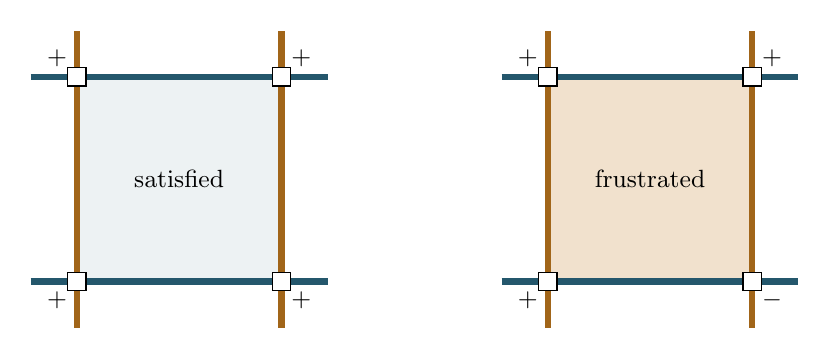
\begin{tikzpicture}[x=13mm,y=13mm,font=\small]
  \foreach \shift/\fr in {0/0,4.6/1}{
    \begin{scope}[shift={(\shift,0)}]
      \ifnum\fr=1 \fill[glowgold!22] (0,0) rectangle (2,2); \else \fill[glowblue!8] (0,0) rectangle (2,2); \fi
      \draw[glowgold!85!black,line width=2.2pt] (0,-.45)--(0,2.45);
      \draw[glowgold!85!black,line width=2.2pt] (2,-.45)--(2,2.45);
      \draw[glowblue,line width=2.2pt] (-.45,2)--(2.45,2);
      \draw[glowblue,line width=2.2pt] (-.45,0)--(2.45,0);
      \foreach \x/\y in {0/0,2/0,0/2,2/2}
        \filldraw[draw=black,fill=white,line width=.5pt] (\x-.09,\y-.09) rectangle (\x+.09,\y+.09);
      \node[above left] at (0,2) {$+$}; \node[above right] at (2,2) {$+$};
      \node[below left] at (0,0) {$+$};
      \ifnum\fr=1 \node[below right] at (2,0) {$-$}; \node at (1,1) {frustrated};
      \else \node[below right] at (2,0) {$+$}; \node at (1,1) {satisfied}; \fi
    \end{scope}}
\end{tikzpicture}
\caption{2 rectangles, with the signs of the couplings at their corners. On the left the 4 couplings can be satisfied by aligning the spins, while on the right one of them must be violated.}\label{fig:frustration}
\end{figure}

The Hadamard condition has a simple interpretation in these terms. For 2 rows $a\neq b$ consider the vector $d_k=H_{ak}H_{bk}$, so that the rectangle with corners $aj,al,bj,bl$ is frustrated when $d_jd_l=-1$. If $d$ has $u$ entries $1$ and $v$ entries $-1$, then the number of frustrated rectangles with sides on the rows $a,b$ is $uv$, and since $u+v=N$, this number is at most $N^2/4$, with equality precisely when $u=v$, that is, when the rows $a,b$ are orthogonal. Thus:

\begin{samepage}
\begin{prop}\label{prop:frustration}
A matrix $H\in M_N(\pm1)$ is Hadamard precisely when, for any $2$ row wires, the number of frustrated rectangles having $2$ of their sides on these wires is $N^2/4$, which is the maximal possible value.
\end{prop}
\end{samepage}

\begin{proof}
This follows from the above discussion, the maximal value of $uv$ subject to $u+v=N$ being attained at $u=v=N/2$, which means $\sum_kH_{ak}H_{bk}=0$.
\end{proof}

In other words, the Hadamard arrays are maximally and uniformly frustrated, at the opposite end from the Mattis ferromagnets of Proposition~\ref{prop:mattis}. For comparison, in a random sign matrix about half of the rectangles are frustrated, while here the proportion is exactly $\frac{N^2/4}{N(N-1)/2}=\frac{N}{2(N-1)}$, slightly more than half, for any 2 rows.

\medskip

\noindent\textbf{Orthogonal couplings.}
Put $\sigma=(a,b)\in\{\pm1\}^{2N}$, and consider the symmetric matrix
\[
 J=\frac{1}{\sqrt N}\begin{pmatrix}0&H\\H^t&0\end{pmatrix}
\]
Then $E=-\frac{1}{2}\langle J\sigma,\sigma\rangle$, so $J$ is the coupling matrix of the $2N$ spins, with no coupling inside the layers. When $H$ is Hadamard we have $J^2=1$, and since $Tr(J)=0$, the eigenvalues of $J$ are $1$ and $-1$, each with multiplicity $N$. This is exactly the spectrum of the couplings in the random orthogonal model of \cite{mp2}, with Hamiltonian $\langle O\sigma,\sigma\rangle$ for a random symmetric orthogonal matrix $O$, discussed in Section~\ref{sec:ising}. In our arrays the orthogonality is not imposed by an averaging, but by the Hadamard condition.

The spectrum of $J$ gives the lower bound for the energy. Since $\|\sigma\|^2=2N$, we have $E\geq-N$, with equality precisely when $J\sigma=\sigma$, that is, when $Hb=\sqrt Na$. In this case all the row sums of the matrix $D_aHD_b$ are equal to $\sqrt N$, and since $\sum_{jk}H_{jk}a_jb_k=N^{3/2}$, so are its column sums. In other words, $D_aHD_b$ is a regular Hadamard matrix, and this requires $N$ to be a square, by integrality.

\begin{samepage}
\begin{defn}
A crystalline state of the Ising array of a Hadamard matrix $H$ is a configuration of energy $-N$, that is, a pair of sign vectors $(a,b)$ such that $D_aHD_b$ has all its row and column sums equal to $\sqrt N$.
\end{defn}
\end{samepage}

The terminology is borrowed from \cite{mp2}, where the sine model is shown to have, when $2N+1$ is prime, a ground state of energy equal to the lower bound, built from a Legendre sequence, and separated from the glassy states by a first order transition. Here the crystalline states are the real bistochastic forms of $H$, studied in \cite{com}.

\medskip

\noindent\textbf{Weighing matrices.} The above makes sense for any matrix $A\in M_N(0,\pm1)$ satisfying $AA^t=w1_N$, called a weighing matrix of weight $w$ \cite{gse}, with couplings $A_{jk}/\sqrt w$. The coupling matrix is then orthogonal, we have $E\geq-N$, and there is equality only if $w$ is a square. The Hadamard matrices are the case $w=N$, and the opposite case, with $w$ of the order of $\log N$, is the fully frustrated hypercube of Marinari, Parisi and Ritort \cite{mp3}:

\begin{samepage}
\begin{prop}\label{prop:hypercube}
Consider signs on the edges of the hypercube $\{0,1\}^D$, and let $A$ be the matrix of the couplings between the $2^{D-1}$ even vertices and the $2^{D-1}$ odd ones. Then all the square faces are frustrated precisely when $AA^t=D1$, that is, when $A$ is a weighing matrix of weight $D$.
\end{prop}
\end{samepage}

\begin{proof}
The hypercube is bipartite, so the couplings are those of an array, given by $A$. The diagonal entries of $AA^t$ are equal to $D$. For 2 even vertices $x\neq z$, the entry $(AA^t)_{xz}$ is a sum over the common neighbors of $x,z$. There are none when $x,z$ are at distance at least 4, and there are 2 of them, $y,y'$, when $x,z$ are at distance 2, in which case $(AA^t)_{xz}=J_{xy}J_{yz}+J_{xy'}J_{y'z}$ vanishes precisely when the face $xyzy'$ is frustrated. Since each face has exactly one diagonal joining even vertices, this gives the result.
\end{proof}

Such signs exist for any $D$, for instance $J_{x,x+e_\nu}=(-1)^{x_1+\ldots+x_{\nu-1}}$, as in \cite{mp3}, and Figure~\ref{fig:cube} shows them for $D=3$, where the program \texttt{pictures.py} checks that the 6 faces are frustrated, and computes $A$. The program \texttt{hypercube.py} checks the above for $D\leq8$, and computes the ground states for $D\leq5$. Thus the fully frustrated hypercube is the Ising array of a weighing matrix of order $2^{D-1}$ and weight $D$, normalized exactly as ours, and the bound of $-1/2$ per spin is reached only when $D$ is a square, as observed in \cite{mp3}.

\begin{figure}[htb!]
\centering
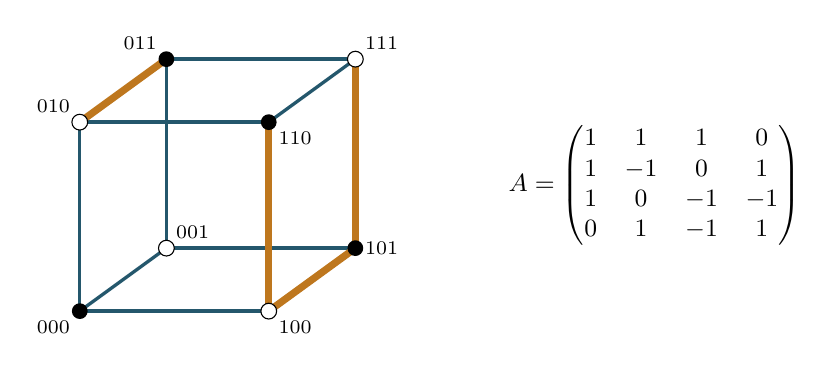
\begin{tikzpicture}[x=10mm,y=10mm,font=\small]
  \foreach \v/\x/\y in {000/0/0,100/2.4/0,010/0/2.4,110/2.4/2.4,001/1.1/.8,101/3.5/.8,011/1.1/3.2,111/3.5/3.2} \coordinate (v\v) at (\x,\y);
  \foreach \p/\q in {000/100,000/010,000/001,001/101,001/011,010/110,011/111,110/111} \draw[glowblue,line width=1.2pt] (v\p)--(v\q);
  \foreach \p/\q in {010/011,100/110,100/101,101/111} \draw[glowgold,line width=2.6pt] (v\p)--(v\q);
  \foreach \v in {000,011,101,110} \fill (v\v) circle (.1);
  \foreach \v in {001,010,100,111} \filldraw[fill=white] (v\v) circle (.1);
  \foreach \v/\a in {000/below left,100/below right,010/above left,110/below right,001/above right,101/right,011/above left,111/above right} \node[\a,font=\scriptsize] at (v\v) {$\v$};
  \node at (7.3,1.6) {$A=\begin{pmatrix}1&1&1&0\\1&-1&0&1\\1&0&-1&-1\\0&1&-1&1\end{pmatrix}$};
\end{tikzpicture}
\caption{The fully frustrated cube, $D=3$, with the positive couplings in blue, and the negative ones drawn thick, in gold, each face having an odd number of them. The even vertices are black, the odd ones white, and the couplings between them form a weighing matrix $A$ of order 4 and weight 3, with rows indexed by $000,011,101,110$, and columns indexed by $001,010,100,111$.}\label{fig:cube}
\end{figure}

The program \texttt{hypercubedos.py} computes the exact densities of states for $D\leq6$, with the C program \texttt{dos.c} of Section~\ref{sec:larger}. It finds the following ground states, with $m=\Omega/(N\sqrt D)$ being the normalized energy, equal to 1 for the crystalline states, and the maximum $c_{max}$ of the specific heat per row wire, defined in Section~\ref{sec:exact}, reached at the temperature $T_{max}$:

\medskip

\begin{center}
\begin{tabular}{|c|c|c|c|c|c|}
\hline
$D$ & $N$ & $m$ & ground states & $c_{max}$ & $T_{max}$\\
\hline
$2$ & $2$ & $1/\sqrt2\simeq0.707$ & $8$ & $0.220$ & $1.179$\\
$3$ & $4$ & $\sqrt3/2\simeq0.866$ & $16$ & $0.341$ & $0.517$\\
$4$ & $8$ & $1$ & $16$ & $0.896$ & $0.371$\\
$5$ & $16$ & $2/\sqrt5\simeq0.894$ & $10240$ & $0.376$ & $0.424$\\
$6$ & $32$ & $9/(4\sqrt6)\simeq0.919$ & $5816320$ & $0.480$ & $0.259$\\
\hline
\end{tabular}
\end{center}

\medskip

For $D=2$ this is the Hadamard matrix of order 2. The bound $m=1$ is reached at $D=4$ only, by 16 crystalline states, and there $T_{max}\simeq0.3705$ is close to the crystallization temperature $T_c\simeq0.3729$ of Section~\ref{sec:exact}. For $D=5,6$ the ground states are frustrated, and very degenerate, and the specific heat only has broad maxima. The Hadamard arrays are the other extreme, of maximal weight. We can now summarize the above, for them, and also introduce the density of states:

\begin{samepage}
\begin{thm}\label{thm:model}
Let $H$ be a real Hadamard matrix of order $N$, and consider its Ising array.
\begin{enumerate}
\item The array is maximally frustrated, in the sense of Proposition~\ref{prop:frustration}.

\item The coupling matrix $J$ is symmetric and orthogonal, with eigenvalues $\pm1$, each of multiplicity $N$, and the energy satisfies $E\geq-N$.

\item There are crystalline states, of energy $-N$, precisely when $H$ is equivalent to a regular Hadamard matrix.

\item The normalized density of states, namely the law of $-E\sqrt N$ under the uniform measure on configurations, is the real glow of $H$, the law of $\Omega=\langle Hb,a\rangle$.
\end{enumerate}
\end{thm}
\end{samepage}

\begin{proof}
All these assertions follow from the above discussion, the last one being a reformulation of the definition of the real glow, from \cite{ba1}.
\end{proof}

\section{The energy levels, 2-adically}\label{sec:2adic}

In this section we look at the density of states modulo powers of 2. It is shown in \cite{ba1} that for $N\geq4$ the law of $\Omega$ is supported by $4\mathbb Z$, and is split $\frac{3}{4}-\frac{1}{4}$ between $8\mathbb Z$ and $8\mathbb Z+4$ when $N=0(8)$, and $\frac{1}{4}-\frac{3}{4}$ when $N=4(8)$, as shown in Figure~\ref{fig:dosfull} for $\mathrm{had}_{16.3}$. The following identity explains this, and shows how to go further.

\begin{figure}[htb!]
\centering
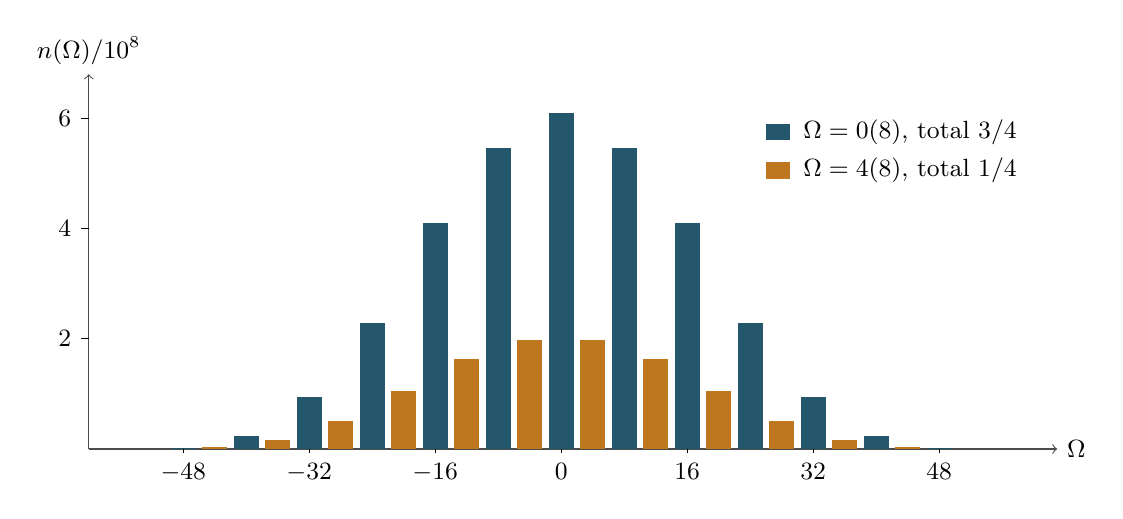
\begin{tikzpicture}[x=1mm,y=7mm,font=\small]
  \draw[->,black!70] (-60,0)--(63,0) node[right,text=black] {$\Omega$};
  \draw[->,black!70] (-60,0)--(-60,6.8) node[above,text=black] {$n(\Omega)/10^8$};
  \foreach \x in {-48,-32,-16,0,16,32,48} \draw (\x,0)--++(0,-.08) node[below] {$\x$};
  \foreach \y in {2,4,6} \draw (-60,\y)--++(-1,0) node[left] {$\y$};
  \foreach \x/\v in {-48/0.026,-40/0.236,-32/0.946,-24/2.285,-16/4.099,-8/5.468,0/6.090,8/5.468,16/4.099,24/2.285,32/0.946,40/0.236,48/0.026} \fill[glowblue] (\x-1.6,0) rectangle (\x+1.6,\v);
  \foreach \x/\v in {-44/0.030,-36/0.171,-28/0.513,-20/1.059,-12/1.626,-4/1.969,4/1.969,12/1.626,20/1.059,28/0.513,36/0.171,44/0.030} \fill[glowgold] (\x-1.6,0) rectangle (\x+1.6,\v);
  \fill[glowblue] (26,5.6) rectangle (29,5.9); \node[right] at (29.5,5.75) {$\Omega=0(8)$, total $3/4$};
  \fill[glowgold] (26,4.9) rectangle (29,5.2); \node[right] at (29.5,5.05) {$\Omega=4(8)$, total $1/4$};
\end{tikzpicture}
\caption{The density of states of $\mathrm{had}_{16.3}$, in units of $10^8$ configurations, with the levels $\Omega=0(8)$ in blue, and the levels $\Omega=4(8)$ in gold. The 2 interlaced profiles carry $3/4$ and $1/4$ of the $4^{16}$ configurations, as for all the Hadamard matrices of order $N=0(8)$.}\label{fig:dosfull}
\end{figure}

\begin{samepage}
\begin{prop}\label{prop:2adic}
Write $H_{jk}=(-1)^{M_{jk}}$, $a_j=(-1)^{\alpha_j}$, $b_k=(-1)^{\beta_k}$, with $M\in M_N(0,1)$ and $\alpha,\beta\in\{0,1\}^N$, and let $\rho=M1$ and $\gamma=M^t1$ be the row and column weights of $M$. Then $\Omega$ equals
\[
 N^2-2|M|-2N(|\alpha|+|\beta|)+4(\langle\alpha,\rho\rangle+\langle\beta,\gamma\rangle+|\alpha||\beta|)-8\langle\alpha,M\beta\rangle
\]
where $|\cdot|$ denotes the sum of entries.
\end{prop}
\end{samepage}

\begin{proof}
We have $\Omega=N^2-2|X|$, where $X_{jk}=M_{jk}\oplus\alpha_j\oplus\beta_k$, and for bits $u,v,w$ we have $u\oplus v\oplus w=u+v+w-2(uv+vw+wu)+4uvw$. Summing over $j,k$ gives the result.
\end{proof}

Thus $\Omega$ modulo 8 only involves linear data, the magnetizations $|\alpha|,|\beta|$ and their overlaps with the weights, while $\Omega$ modulo 16 involves the bilinear form $\langle\alpha,M\beta\rangle$ over $\mathbb F_2$, $\Omega$ modulo 32 involves the same form over $\mathbb Z_4$, and so on. In short, the energy is a 2-adic tower of bilinear forms. When $16|N$ the 2nd level has a neat formulation, as a partition function at an imaginary temperature:

\begin{samepage}
\begin{prop}\label{prop:imaginary}
Assume $16|N$, and that $H$ is dephased, with first row and column positive. Then
\[
 P(\Omega=4(16))=P(\Omega=12(16))=\frac{1}{8}\quad,\quad P(\Omega=0(16))-P(\Omega=8(16))=E\left(i^{\langle\alpha,H\beta\rangle}\right)
\]
with $\alpha,\beta\in\{0,1\}^N$ uniform on the right, this latter quantity being real.
\end{prop}
\end{samepage}

\begin{proof}
For $H$ dephased we have $\rho=\gamma=(0,N/2,\ldots,N/2)$ and $|M|=N(N-1)/2$. Since $16|N$, all the terms in Proposition~\ref{prop:2adic} vanish modulo 16, except for the last 2, so $\Omega=4|\alpha||\beta|-8\langle\alpha,M\beta\rangle\,(16)$. When $|\alpha||\beta|$ is odd, which happens with probability $\frac{1}{4}$, we have $\Omega=4,12(16)$, and these 2 values are equally likely, because $a\to-a$ maps $\Omega\to-\Omega$. When $|\alpha||\beta|$ is even we have $\Omega/8=|\alpha||\beta|/2+\langle\alpha,M\beta\rangle\,(2)$, and so
\[
 P(\Omega=0(16))-P(\Omega=8(16))=Re\,E\left(i^{|\alpha||\beta|+2\langle\alpha,M\beta\rangle}\right)
\]
because the real part vanishes when $|\alpha||\beta|$ is odd. Now $|\alpha||\beta|+2\langle\alpha,M\beta\rangle=\sum_{jk}(1+2M_{jk})\alpha_j\beta_k$, and $1+2M_{jk}=H_{jk}\,(4)$, which gives the formula. Finally, replacing $\alpha$ by $1-\alpha$ changes $\langle\alpha,H\beta\rangle$ into $N\beta_1-\langle\alpha,H\beta\rangle$, because the column sums of $H$ are $N,0,\ldots,0$, so the expectation equals its conjugate.
\end{proof}

The real Hadamard matrices of order $N\leq20$ that we use are taken from McKay's catalogue \cite{mck}, and are in the folder \texttt{matrices} of the code, together with the Paley matrix of order 12. At $N=16$, the program \texttt{glowlaw.py} computes the exact densities of states, for all the 5 classes, by grouping the vectors $b$ according to the multiset of the numbers $|(Hb)_j|$, which determines the law of $\Omega$ over $a$. The program \texttt{twoadic.py} then computes the residues modulo 16, and checks Proposition~\ref{prop:imaginary} by computing the right hand side independently, via $E(i^{\langle\alpha,H\beta\rangle})=E_\beta\prod_j\frac{1+i^{(H\beta)_j}}{2}$. We obtain the following table, where $p_x=P(\Omega=x(16))$, and where $r$ is the 2-rank of the core of the dephased binary matrix, as in the introduction:

\medskip

\begin{center}
\begin{tabular}{|l|c|c|c|c|}
\hline
$H$ & $r$ & $p_4=p_{12}$ & $p_0-p_8$ & $2^{-8}+2^{-2-r}$\\
\hline
$\mathrm{had}_{16.0}=W_{16}$ & $4$ & $1/8$ & $5/256$ & $5/256$\\
$\mathrm{had}_{16.1}$ & $5$ & $1/8$ & $3/256$ & $3/256$\\
$\mathrm{had}_{16.2}$ & $6$ & $1/8$ & $2/256$ & $2/256$\\
$\mathrm{had}_{16.3}$ & $7$ & $1/8$ & $3/512$ & $3/512$\\
$\mathrm{had}_{16.4}$ & $7$ & $1/8$ & $3/512$ & $3/512$\\
\hline
\end{tabular}
\end{center}

\medskip

At the other orders, Proposition~\ref{prop:2adic} with the values of $\rho,\gamma,|M|$ from the above proof gives $\Omega=N(1-2\alpha_1-2\beta_1)+4|\alpha||\beta|-8\langle\alpha,M\beta\rangle$, for $H$ dephased, and the same argument shows that, with $n=N/4$, we have
\[
 p_0-p_8=i^nE\left((-1)^{n(\alpha_1+\beta_1)}i^{\langle\alpha,H\beta\rangle}\right)
\]
The program \texttt{residues.py} checks this for $N\leq20$, and computes the law modulo 16 at all the orders where we know the densities of states, namely for all the classes with $N\leq28$, from Sections~\ref{sec:exact} and \ref{sec:larger}, and for the 360 matrices of order 32 and the 9 regular matrices of order 36 of Section~\ref{sec:larger}. We obtain the following table, where the 2-rank $r$ takes all the values from 4 to 7 at $N=16$, and from 5 to 15 at $N=32$:

\medskip

\begin{center}
\begin{tabular}{|c|c|c|c|c|}
\hline
$N$ & matrices & $r$ & $p_4=p_{12}$ & $p_0-p_8$\\
\hline
$4$ & $1$ & $2$ & $3/8$ & $2^{-3}$\\
$8$ & $1$ & $3$ & $1/8$ & $-3\cdot2^{-5}$\\
$12$ & $1$ & $10$ & $3/8$ & $-2^{-7}$\\
$16$ & $5$ & $4$--$7$ & $1/8$ & $2^{-8}+2^{-2-r}$\\
$20$ & $3$ & $18$ & $3/8$ & $2^{-11}$\\
$24$ & $60$ & $11$ & $1/8$ & $-3\cdot2^{-13}$\\
$28$ & $487$ & $26$ & $3/8$ & $-2^{-15}$\\
$32$ & $360$ & $5$--$15$ & $1/8$ & $2^{-16}+2^{-2-r}$\\
$36$ & $9$ & $34$ & $3/8$ & $2^{-19}$\\
\hline
\end{tabular}
\end{center}

\medskip

Thus $p_0-p_8=(-1)^{(N-4)/8}2^{-N/2-1}$ for $N=4(8)$, and $p_0-p_8=(-1)^{N/8}(2^{-N/2}+2^{-2-r})$ for $N=0(8)$, for all these matrices. As for the 2-rank, it is $N-2$ for $N=4(8)$, and $N/2-1$ for $N=8(16)$, the latter value corresponding to the fact that the binary code of $H$, spanned by the rows of the 0-1 matrix obtained by replacing the entries $-1$ of $H$ by 0, which has dimension $r+1$, is self-dual \cite{hcb}. In short, the law modulo 16 only varies with $H$ at the orders $N=0(16)$, as illustrated in Figure~\ref{fig:residues}. All this can be proved, by computing the above partition functions at imaginary temperature, as follows:

\begin{figure}[htb!]
\centering
\begin{tikzpicture}[x=3mm,y=3mm,font=\small]
  \draw[->,black!70] (0,0)--(39,0) node[right,text=black] {$N$};
  \draw[->,black!70] (0,0)--(0,21) node[above,text=black] {$-\log_2|p_0-p_8|$};
  \foreach \x in {4,8,...,36} \draw (\x,0)--++(0,-.3) node[below] {$\x$};
  \foreach \y in {5,10,15,20} \draw (0,\y)--++(-.3,0) node[left] {$\y$};
  \draw[black!40,densely dashed] (2,2)--(38,20) node[right,text=black!60] {$N/2+1$};
  \foreach \x/\y in {4/3.000,16/5.678,16/6.415,16/7.000,16/7.415,20/11.000,32/6.997,32/7.994,32/8.989,32/9.978,32/10.956,32/11.913,32/12.830,32/13.678,32/14.415,32/15.000,32/15.415,36/19.000} \fill[glowblue] (\x,\y) circle (.28);
  \foreach \x/\y in {8/3.415,12/7.000,24/11.415,28/15.000} \fill[glowgold] (\x,\y) circle (.28);
  \node[right,font=\scriptsize] at (32.4,6.997) {$r=5$}; \node[right,font=\scriptsize] at (32.4,15.415) {$r=15$};
  \node[left,font=\scriptsize] at (15.6,5.678) {$r=4$}; \node[left,font=\scriptsize] at (15.6,7.415) {$r=7$};
  \fill[glowblue] (3,18) circle (.28); \node[right] at (3.5,18) {$p_0>p_8$};
  \fill[glowgold] (3,16) circle (.28); \node[right] at (3.5,16) {$p_0<p_8$};
\end{tikzpicture}
\caption{The values of $-\log_2|p_0-p_8|$, at all the orders where we know the densities of states. The dashed line $N/2+1$ is reached at $N=4(8)$, the points at $N=8(16)$ are $\log_23$ below it, and at $N=16,32$ the values depend on the 2-rank $r$, which takes the values $4,\ldots,7$ and $5,\ldots,15$.}\label{fig:residues}
\end{figure}

\begin{samepage}
\begin{lem}\label{lem:gauss}
Let $H$ be a dephased Hadamard matrix of order $N\geq4$, write $H=(-1)^M$ with $M\in M_N(0,1)$, and let $r$ be the $2$-rank of $M$. With $\alpha,\beta\in\{0,1\}^N$ uniform, we have $E(i^{\langle\alpha,H\beta\rangle})=2^{-N/2}+2^{-2-r}$ when $N=0(8)$, and $E((-1)^{\alpha_1+\beta_1}i^{\langle\alpha,H\beta\rangle})=-i\cdot2^{-N/2-1}$ when $N=4(8)$.
\end{lem}
\end{samepage}

\begin{proof}
Since $H_{jk}=1+2M_{jk}\,(4)$, we have $i^{\langle\alpha,H\beta\rangle}=i^{|\alpha||\beta|}(-1)^{\langle\alpha,M\beta\rangle}$. Let $v\in\{0,1\}^N$ be the sum modulo 2 of the rows of $M$ selected by $\alpha$. The rows of $M$ other than the first one have $N/2$ entries 1, any 2 of them having $N/4$ common entries 1, by orthogonality, so by inclusion-exclusion, if $s$ of them are selected, the weight of $v$ is $|v|=sN/2-s(s-1)N/4\,(4)$. Thus $|v|=0(4)$ when $N=0(8)$, and $|v|=s(3-s)\,(4)$ when $N=4(8)$. Now for $t\in\{0,1\}$, and $u=v+te_1$, summing over $\beta$ gives
\[
 E_\beta\left(i^{|\alpha||\beta|}(-1)^{\langle u,\beta\rangle}\right)=\prod_k\frac{1+i^{|\alpha|}(-1)^{u_k}}{2}
\]
which is $[u=0]$ for $|\alpha|=0(4)$, is $[u=1]$ for $|\alpha|=2(4)$, where $1$ is the all-one vector, and is $2^{-N/2}e^{i\pi\varepsilon(N-2|u|)/4}$ for $|\alpha|$ odd, where $i^{|\alpha|}=i\varepsilon$.

For $N=0(8)$ we take $t=0$. Since $v_1=0$, the case $u=1$ never occurs, and for $|\alpha|$ odd the above quantity is $2^{-N/2}$, because $e^{i\pi N/4}=1$ and $|v|=0(4)$. The vectors $\alpha$ with $v=0$ form a binary code $K$ of dimension $N-r$, whose orthogonal $K^\perp$ is spanned by the columns of $M$, so that the elements of $K^\perp$ have weights $0(4)$, by the above argument for $H^t$. By the Poisson summation formula, we obtain
\[
 \sum_{\alpha\in K}i^{|\alpha|}=\frac{|K|}{2^N}\sum_{w\in K^\perp}\prod_k\left(1+i(-1)^{w_k}\right)=\frac{|K|}{2^N}\sum_{w\in K^\perp}2^{N/2}i^{-|w|}=2^{N/2}
\]
Since $e_1\in K$, half of the elements of $K$ have odd weight, so $K$ has $(|K|+2^{N/2+1})/4$ elements of weight $0(4)$. Thus $E(i^{\langle\alpha,H\beta\rangle})=2^{-N}(2^{N-r-2}+2^{N/2-1})+2^{-N/2-1}$, as stated.

For $N=4(8)$ we take $t=1$, and multiply by $(-1)^{\alpha_1}$. Here $u_1=1$, so $u\neq0$, and $u=1$ would mean $|v|=N-1$, which is odd, so only the vectors $\alpha$ of odd weight contribute, and since $e^{i\pi\varepsilon N/4}=-1$, the contribution of $\alpha$ is $-2^{-N/2}(-1)^{\alpha_1}i^{-\varepsilon(|v|+1)}$. With $s=|\alpha|-\alpha_1$, which is odd when $\alpha_1=0$, and even when $\alpha_1=1$, the formula $|v|=s(3-s)\,(4)$ shows that $(-1)^{\alpha_1}i^{-\varepsilon(|v|+1)}=i$ in all the 4 cases for $s$ modulo 4. Thus the expectation is $-\frac{1}{2}\cdot2^{-N/2}i$, as stated.
\end{proof}

Now back to the densities of states, we obtain the following result, which at $N=16$ is a shadow of a much more precise statement, Theorem~\ref{intro:spectrum}, describing the full densities of states, as we will see in Section~\ref{sec:exact}, the next step being to go up the 2-adic tower:

\begin{samepage}
\begin{thm}\label{thm:2adic}
Let $H$ be a real Hadamard matrix of order $N\geq4$, and $r$ the $2$-rank of the core of its dephased binary matrix. With $p_x=P(\Omega=x(16))$ we have $p_4=p_{12}$, and
\[
 p_0-p_8=\begin{cases}
 (-1)^{N/8}(2^{-N/2}+2^{-2-r})&{\rm if}\ N=0(8)\\
 (-1)^{(N-4)/8}2^{-N/2-1}&{\rm if}\ N=4(8)
 \end{cases}
\]
so that the law of the real glow modulo $16$ is determined by $N$ and $r$. At $N=16$ we have $p_4=p_{12}=\frac{1}{8}$ and $p_0-p_8=2^{-8}+2^{-2-r}$, for all $5$ classes.
\end{thm}
\end{samepage}

\begin{proof}
Since the density of states only depends on the equivalence class of $H$, we can assume that $H$ is dephased. Since $a\to-a$ maps $\Omega\to-\Omega$, we have $p_4=p_{12}$, and since $\Omega\in4\mathbb Z$, we have $p_0-p_8=E(i^{\Omega/4})$. By the formula for $\Omega$ before the table, we have $i^{\Omega/4}=i^n(-1)^{n(\alpha_1+\beta_1)}i^{\langle\alpha,H\beta\rangle}$, with $n=N/4$, and Lemma~\ref{lem:gauss} gives the result, with $i^n=(-1)^{N/8}$ when $N=0(8)$, and $i^n\cdot(-i)=(-1)^{(N-4)/8}$ when $N=4(8)$. The law modulo 16 is then determined, because the law of $\Omega$ modulo 8 is known from \cite{ba1}. At $N=16$ this is the above computation, the 5 classes being all the Hadamard matrices of order 16, up to equivalence \cite{hal}.
\end{proof}

\section{Universal moments and the 4-profile}\label{sec:moments}

We now look at the moments of the density of states, $E(\Omega^{2p})$, the odd ones being zero, because $a\to-a$ maps $\Omega\to-\Omega$. These moments are the coefficients of the high-temperature expansion of the partition function $Z_H(\beta)=4^NE(e^{\beta\Omega/\sqrt N})$. We use cumulants, because the free energy is their generating function.

\medskip

\noindent\textbf{Graphs.}
For a uniform random sign $u$ we have $E(e^{tu})=\cosh t$, and the cumulants $c_m$ of $u$ are the coefficients of $\log\cosh t=\sum_mc_mt^m/m!$, namely $c_2=1$, $c_4=-2$, $c_6=16$, $c_8=-272$, the odd ones being 0. Consider the $2p$ factors of $\Omega^{2p}$ as $2p$ positions, and take a partition $\pi$ of these positions for the row indices, and a partition $\rho$ for the column indices. This gives a bipartite multigraph $D_{\pi\rho}$, whose row vertices are the blocks of $\pi$, whose column vertices are the blocks of $\rho$, and with an edge for each position, joining its 2 blocks. The free contraction of a matrix $A\in M_N(\mathbb R)$ along this graph is
\[
 S_{\pi\rho}(A)=\sum_{x,y}\prod_{s=1}^{2p}A_{x(s)y(s)}
\]
the sum being over all labelings $x$ of the row vertices and $y$ of the column vertices by $1,\ldots,N$, not necessarily injective, with $x(s),y(s)$ being the labels of the 2 ends of the edge $s$.

\begin{samepage}
\begin{lem}\label{lem:graphs}
For $A\in M_N(\mathbb R)$ and $\Omega_A=\langle Ab,a\rangle$, with $a,b$ uniform sign vectors, we have
\[
 E(\Omega_A^{2p})=\sum_{\pi,\rho}c_\pi c_\rho\,S_{\pi\rho}(A)\quad,\quad\kappa_{2p}(\Omega_A)=\sum_{\pi,\rho\ \mathrm{connected}}c_\pi c_\rho\,S_{\pi\rho}(A)
\]
where $c_\pi=\prod_{B\in\pi}c_{|B|}$, the 2nd sum being over the pairs whose graph is connected.
\end{lem}
\end{samepage}

\begin{proof}
For fixed labels, the moment-cumulant formula gives $E(a_{x_1}\ldots a_{x_{2p}})=\sum_\pi\prod_Bc_{|B|}$, the sum being over the partitions $\pi$ such that $x$ is constant on the blocks, because the joint cumulants of independent variables vanish unless all the variables coincide. Doing the same for $b$, and summing over the labels, gives the first formula. The 2nd one follows from the first by the formula of Leonov and Shiryaev for the cumulants of products \cite{lsh}, exactly as in the complex case, explained in \cite{cot}.
\end{proof}

\begin{figure}[htb!]
\centering
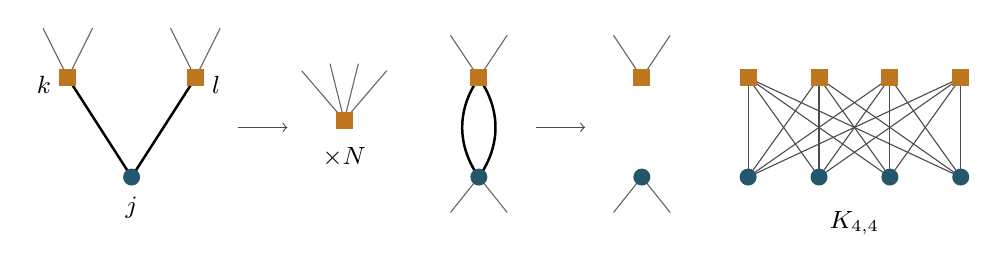
\begin{tikzpicture}[x=9mm,y=9mm,font=\small]
  \draw[black!60] (0,2)--(-.35,2.7) (0,2)--(.35,2.7) (1.8,2)--(1.45,2.7) (1.8,2)--(2.15,2.7);
  \draw[line width=.9pt] (0,2)--(.9,.6)--(1.8,2);
  \fill[glowblue] (.9,.6) circle (.12);
  \fill[glowgold] (-.12,1.88) rectangle (.12,2.12); \fill[glowgold] (1.68,1.88) rectangle (1.92,2.12);
  \node[below] at (.9,.45) {$j$}; \node[left] at (-.1,1.9) {$k$}; \node[right] at (1.9,1.9) {$l$};
  \draw[->,black!70] (2.4,1.3)--(3.1,1.3);
  \draw[black!60] (3.9,1.4)--(3.3,2.1) (3.9,1.4)--(3.7,2.2) (3.9,1.4)--(4.1,2.2) (3.9,1.4)--(4.5,2.1);
  \fill[glowgold] (3.78,1.28) rectangle (4.02,1.52);
  \node[below] at (3.9,1.15) {$\times N$};
  \begin{scope}[shift={(5.8,0)}]
    \draw[black!60] (0,.6)--(-.4,.1) (0,.6)--(.4,.1) (0,2)--(-.4,2.6) (0,2)--(.4,2.6);
    \draw[line width=.9pt] (0,.6) to[bend left=35] (0,2); \draw[line width=.9pt] (0,.6) to[bend right=35] (0,2);
    \fill[glowblue] (0,.6) circle (.12); \fill[glowgold] (-.12,1.88) rectangle (.12,2.12);
    \draw[->,black!70] (.8,1.3)--(1.5,1.3);
    \draw[black!60] (2.3,.6)--(1.9,.1) (2.3,.6)--(2.7,.1) (2.3,2)--(1.9,2.6) (2.3,2)--(2.7,2.6);
    \fill[glowblue] (2.3,.6) circle (.12); \fill[glowgold] (2.18,1.88) rectangle (2.42,2.12);
  \end{scope}
  \begin{scope}[shift={(9.6,0)}]
    \foreach \i in {0,...,3} \foreach \k in {0,...,3} \draw[black!70] (\i,.6)--(\k,2);
    \foreach \i in {0,...,3} {\fill[glowblue] (\i,.6) circle (.12); \fill[glowgold] (\i-.12,1.88) rectangle (\i+.12,2.12);}
    \node at (1.5,-.05) {$K_{4,4}$};
  \end{scope}
\end{tikzpicture}
\caption{The reduction rules for the graphs of Lemma~\ref{lem:graphs}, at $A=H$, with the row vertices in blue, and the column vertices in gold. On the left, a vertex of degree 2 is removed, with a factor $N$, and its 2 neighbors are identified. In the middle, a pair of parallel edges is removed. On the right, the graph $K_{4,4}$, which survives the reduction, and produces the 4-profile at order 16.}\label{fig:graphs}
\end{figure}

When $AA^t=A^tA=N1_N$, as is the case for $A=H$, a vertex of degree 2 can be removed: if its 2 neighbors have labels $k,l$, summing over its label gives $\sum_jA_{jk}A_{jl}=N\delta_{kl}$, so we can remove the vertex, multiply by $N$, and identify its 2 neighbors. When $A$ has entries $\pm1$, a pair of parallel edges can be removed too, because $A_{jk}^2=1$, and an isolated vertex contributes a factor $N$. Applying these rules as long as possible, we end up with a simple graph whose vertices all have even degree, either 0 or at least 4. Now a simple bipartite graph whose vertices have degree at least 4 has at least 4 vertices on each side, and therefore at least 16 edges, with equality only for the complete bipartite graph $K_{4,4}$, shown in Figure~\ref{fig:graphs}, together with the reduction rules. This gives:

\begin{samepage}
\begin{thm}\label{thm:moments}
Let $H$ be a real Hadamard matrix of order $N$.
\begin{enumerate}
\item For $p\leq7$, the moment $E(\Omega^{2p})$ is given by a polynomial $U_p(N)$, which is the same for all real Hadamard matrices, including those of order $1,2$.

\item We have $\kappa_2=N^2$, $\kappa_4=-6N^3+4N^2$, $\kappa_6=240N^4-480N^3+256N^2$, and $\kappa_8=-25200N^5+104160N^4-153216N^3+73984N^2$.

\item At order $16$ we have $E(\Omega^{16})=U_8(N)+\frac{2^8\,16!}{4!}\,P_4(H)$, with $U_8$ a polynomial, where $P_4(H)$ is the sum, over the sets $I$ of $4$ rows, of $(\sum_k\prod_{j\in I}H_{jk})^4$.
\end{enumerate}
\end{thm}
\end{samepage}

\begin{proof}
(1) By Lemma~\ref{lem:graphs}, the moment is a finite sum of contractions along graphs with $2p\leq14$ edges, and by the above discussion, each of them reduces to a power of $N$.

(2) For the cumulants, the connected graphs give at most $N^{p+1}$, as explained in Section~\ref{sec:free} below, so $\kappa_{2p}$ is a polynomial of degree at most $p+1$. The program \texttt{universal.py} computes it by interpolation, from the exact moments at $N=1,2,4,8,12,16,20$, computed by \texttt{glowlaw.py} and \texttt{moments.py}, the polynomials of degree at most 5 being then checked on the remaining orders.

(3) At $2p=16$ the reduction ends with a power of $N$, except for the graphs which are already $K_{4,4}$, with no reduction possible. These graphs correspond to the arrangements of the 16 positions in a $4\times4$ grid, up to permutations of the rows and of the columns of the grid, so there are $16!/(4!)^2$ of them, all with weight $c_4^8=2^8$. Their contraction is
\[
 S_{K_{4,4}}(H)=\sum_{j_1,\ldots,j_4}\Big(\sum_k\prod_{s=1}^4H_{j_sk}\Big)^4
\]
and the terms with distinct indices give $4!\,P_4(H)$, while those with $j_s=j_t$ for some $s\neq t$ reduce to powers of $N$, because $H_{jk}^2=1$, and the rows are orthogonal. Thus the dependence on $H$ is $2^8\cdot\frac{16!}{(4!)^2}\cdot4!\,P_4(H)$, as stated.
\end{proof}

Here $E(\Omega^2)=N^2$ and $E(\Omega^4)=3N^4-6N^3+4N^2$ give $\kappa_2$ and $\kappa_4$, and for instance $E(\Omega^6)=15N^6-90N^5+300N^4-480N^3+256N^2$. As a check, the program \texttt{moments.py} verifies, in exact rational arithmetic, that the 5 classes of order 16 have the same moments up to $E(\Omega^{14})$, and that their 16th moments differ as predicted by (3).

\medskip

\noindent\textbf{The 4-profile.}
The distribution of the numbers $|\sum_k\prod_{j\in I}H_{jk}|$, over the sets $I$ of 4 rows, is the 4-profile of Cooper, Milas and Wallis \cite{cmw}, a classical invariant for the equivalence of Hadamard matrices, and $P_4(H)$ is the sum of their 4th powers. With $p=\sum_k\prod_{j\in I}H_{jk}$ we have $p=N(8)$, and at $N=16$ the possible values are $p=0,\pm8,\pm16$, the value $\pm16$ meaning that the product of the 4 rows is constant. The program \texttt{moments.py} finds the following numbers of sets of 4 rows with each absolute value:

\medskip

\begin{center}
\begin{tabular}{|l|c|c|c|c|}
\hline
$H$ & $|p|=0$ & $|p|=8$ & $|p|=16$ & $r$\\
\hline
$\mathrm{had}_{16.0}=W_{16}$ & $1680$ & $0$ & $140$ & $4$\\
$\mathrm{had}_{16.1}$ & $1488$ & $256$ & $76$ & $5$\\
$\mathrm{had}_{16.2}$ & $1392$ & $384$ & $44$ & $6$\\
$\mathrm{had}_{16.3},\mathrm{had}_{16.4}$ & $1344$ & $448$ & $28$ & $7$\\
\hline
\end{tabular}
\end{center}

\medskip

Thus the number of sets of 4 rows with constant product is $12+2^{11-r}$, and the 4-profile is a function of the 2-rank. At $N=20$ the 3 classes have the same 4-profile, with $4560$ sets of 4 rows with $|p|=4$, and $285$ with $|p|=12$. Since the sum of $p^2$ over the sets of 4 rows is universal, by the same argument as in the proof of Theorem~\ref{thm:moments}, at $N=16$ the 16th moment only depends on the number of sets with $|p|=16$. Summarizing, we have:

\begin{samepage}
\begin{thm}\label{thm:profile}
At $N=16$, the moments of the density of states of the Ising array coincide up to order $14$, and the $16$th moments are given by
\[
 E(\Omega^{16})=E_{16.3}(\Omega^{16})+2^{19}\cdot16!\,(2^{11-r}-16)
\]
with $E_{16.3}$ denoting the moments of $\mathrm{had}_{16.3}$. At $N=20$, all the moments of the $3$ classes coincide.
\end{thm}
\end{samepage}

\begin{proof}
The difference of 16th moments is $\frac{2^8\,16!}{4!}$ times the difference of the numbers $P_4$, which is $(16^4-4\cdot8^4)\,(2^{11-r}-16)=49152\,(2^{11-r}-16)$, by the table, the constraint on the sum of $p^2$ forcing the numbers with $|p|=8$ to decrease by 4 when those with $|p|=16$ increase by 1. Since $49152\cdot2^8/24=2^{19}$, this gives the formula. The statement at $N=20$ follows from the coincidence of the densities of states, found in Section~\ref{sec:exact}.
\end{proof}

\section{The free energy at high temperature}\label{sec:free}

As explained in Section~\ref{sec:ising}, Marinari, Parisi and Ritort observed that the high-temperature expansion of a model with orthogonal couplings only uses their orthogonality, and coincides with the one of a random orthogonal matrix \cite{mp1,mp2}. We will now prove this for our arrays, at leading order, along the lines of the complex case treated in \cite{cot}.

\medskip

\noindent\textbf{The leading term.}
At a vertex of degree 2 the reduction rule of Section~\ref{sec:moments} only uses $AA^t=A^tA=N1_N$, and not the fact that the entries are signs. For a connected graph with $2k$ edges, apply this rule as long as possible. If the graph reduces to a single vertex, its contraction is exactly $N^{k+1}$, with $k$ factors $N$ coming from the reductions, and one from the remaining free label. Otherwise, after $k-s$ reductions there remain $2s$ edges, with $s\geq1$, and all the remaining vertices have degree at least 4, so their number $v$ satisfies $4v\leq4s$. For $A=H$ all the products of entries have modulus 1, so the contraction is bounded by $N^{k-s}N^v\leq N^k$. Thus:
\[
 \kappa_{2k}(\Omega_H)=L_kN^{k+1}+O_k(N^k)
\]
uniformly in $H$, where $L_k$ is the total weight of the connected graphs which reduce completely, and which does not depend on $H$.

\medskip

\noindent\textbf{The Haar orthogonal computation.}
To compute $L_k$, we use the same graphs with $A=\sqrt NO$, where $O$ is a Haar orthogonal matrix, independent of $a,b$. A column of $O$ is uniform on the sphere, and its first coordinate $x$ satisfies $E(x^{2m})=\frac{(2m-1)!!}{N(N+2)\ldots(N+2m-2)}$. In particular the entries of $A$ have bounded moments, and the degree 2 rule holds exactly for $A$. The graphs which do not reduce completely contribute $O_k(N^k)$ in every $L^p$ norm, by H\"older's inequality. More precisely, with $K_j(O)$ being the $j$th cumulant of $\Omega_A$ at fixed $O$, we have $K_{2j}(O)=L_jN^{j+1}+R_j$ with $\|R_j\|_{L^p}=O_{j,p}(N^j)$, and the law of total cumulance expresses $\kappa_{2k}(\Omega_A)$ as a sum over set partitions of joint cumulants of the variables $K_{|B|}(O)$. In the terms with at least 2 blocks the constants $L_jN^{j+1}$ disappear, the odd $K_j$ vanish, and the H\"older inequality bounds these terms by $O_k(N^k)$, while the one-block term carries $L_kN^{k+1}$. Thus, exactly as in \cite{cot}, we obtain, coefficientwise:
\[
 \frac{1}{N}\log E_OE\left(e^{\beta\Omega_A/\sqrt N}\right)\to\sum_k\frac{L_k\beta^{2k}}{(2k)!}
\]
On the other hand, for fixed $a,b$, which have norm $\sqrt N$, the variable $\Omega_A/\sqrt N=\langle Ob,a\rangle$ has the law of $Nx$, by invariance of the Haar measure. With $M=N/2$ and $(M)_m=M(M+1)\ldots(M+m-1)$, this gives
\[
 E_OE\left(e^{\beta\Omega_A/\sqrt N}\right)=\sum_m\frac{\beta^{2m}N^{2m}(2m-1)!!}{(2m)!\,N(N+2)\ldots(N+2m-2)}=\sum_m\frac{M^{2m}\beta^{2m}}{m!\,(M)_m}
\]
which is the series $F_M(\beta^2)$ of \cite{cot}, for which it is shown there that $M^{-1}\log F_M(x)\to\Phi_0(x)$ coefficientwise, with
\[
 \Phi_0(x)=\sqrt{1+4x}-1-\log\frac{1+\sqrt{1+4x}}{2}
\]
Since $N=2M$, we obtain $\sum_kL_k\beta^{2k}/(2k)!=\Phi_0(\beta^2)/2$, and since the coefficients of $\Phi_0$ are $(-1)^{k-1}Cat_{k-1}/k$, we obtain $L_k=(-1)^{k-1}(2k-1)!\,Cat_{k-1}$. For instance $L_1,L_2,L_3,L_4=1,-6,240,-25200$, in agreement with Theorem~\ref{thm:moments}.

\medskip

\noindent\textbf{Thermodynamics.}
Put $\Psi(\beta)=\Phi_0(\beta^2)/2$. Then $N^{-1}\log Z_H(\beta)\to2\log2+\Psi(\beta)$, coefficientwise, so the predicted free energy per row wire is $-(2\log2+\Psi(\beta))/\beta$. The mean energy per row wire, divided by the ground state bound $-1$, is
\[
 m(\beta)=\Psi'(\beta)=\frac{\sqrt{1+4\beta^2}-1}{2\beta}
\]
which is the energy curve $\beta/(1+\sqrt{1+\beta^2})$ of the complex arrays in \cite{cot}, at the doubled inverse temperature $2\beta$. The entropy per row wire is
\[
 s(\beta)=2\log2+\Psi(\beta)-\beta\Psi'(\beta)=2\log2-\frac{1}{2}\log\frac{1+\sqrt{1+4\beta^2}}{2}
\]
which decreases from $2\log2$ at $\beta=0$, and vanishes when $1+\sqrt{1+4\beta^2}=32$, that is, at $\beta=\sqrt{240}\simeq15.49$, where $m=\sqrt{15}/4\simeq0.968$. Since the entropy of Ising spins cannot be negative, the paramagnetic solution must break down before, as in the random energy model of Derrida \cite{der}. Figure~\ref{fig:entropy}, computed by \texttt{pictures.py}, shows how the exact arrays avoid this, their entropies tending at low temperature to the ground state entropies, which are positive, and dropping sharply at the crystallization temperature, for the regular matrices.

\begin{figure}[htb!]
\centering
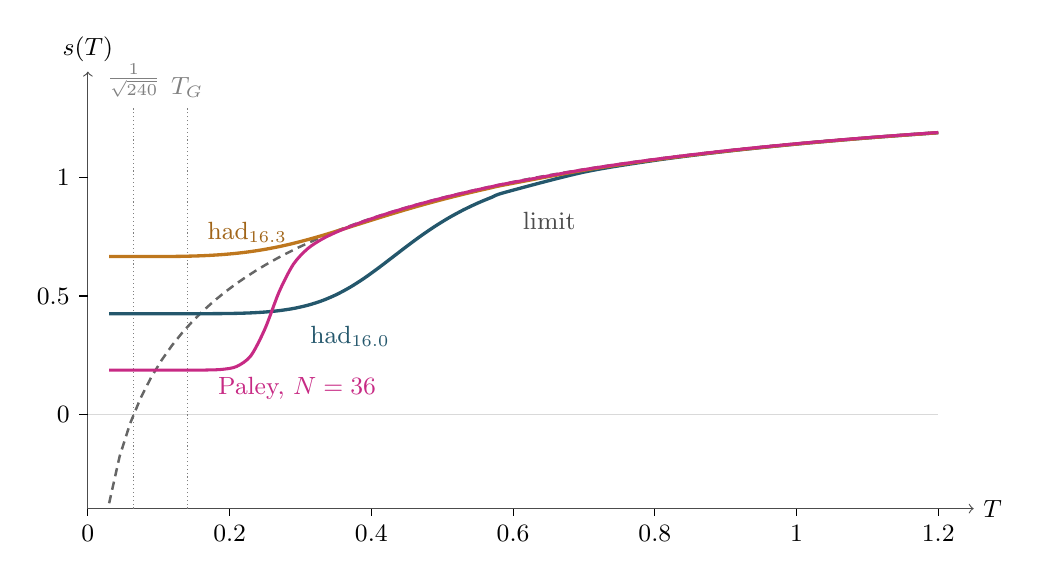
\begin{tikzpicture}[x=90mm,y=30mm,font=\small]
  \draw[black!15] (0,0)--(1.2,0);
  \draw[->,black!70] (0,-.4)--(1.25,-.4) node[right,text=black] {$T$};
  \draw[->,black!70] (0,-.4)--(0,1.45) node[above,text=black] {$s(T)$};
  \foreach \x in {0,0.2,0.4,0.6,0.8,1,1.2} \draw (\x,-.4)--++(0,-.03) node[below] {$\x$};
  \foreach \y in {0,0.5,1} \draw (0,\y)--++(-.012,0) node[left] {$\y$};
  \draw[black!50,densely dotted] (0.0645,-.4)--(0.0645,1.3) node[above] {$\frac{1}{\sqrt{240}}$};
  \draw[black!50,densely dotted] (0.14,-.4)--(0.14,1.3) node[above] {$T_G$};
  \draw[black!60,densely dashed,line width=.9pt] plot[domain=0.03:1.2,samples=80] (\x,{2*ln(2)-0.5*ln((1+sqrt(1+4/(\x*\x)))/2)});
  \draw[glowblue,line width=1.2pt] plot[smooth] coordinates {(0.03,0.4249) (0.05,0.4249) (0.07,0.4249) (0.09,0.4249) (0.11,0.4249) (0.13,0.4249) (0.15,0.4249) (0.17,0.4251) (0.19,0.4255) (0.21,0.4265) (0.23,0.4285) (0.25,0.4321) (0.27,0.4380) (0.29,0.4471) (0.31,0.4606) (0.33,0.4795) (0.35,0.5049) (0.37,0.5370) (0.39,0.5754) (0.41,0.6186) (0.43,0.6643) (0.45,0.7103) (0.47,0.7545) (0.49,0.7953) (0.51,0.8321) (0.53,0.8646) (0.55,0.8931) (0.57,0.9180) (0.59,0.9399) (0.7,1.0244) (0.8,1.0741) (0.9,1.1121) (1,1.1431) (1.1,1.1691) (1.2,1.1913)};
  \draw[glowgold,line width=1.2pt] plot[smooth] coordinates {(0.03,0.6668) (0.05,0.6668) (0.07,0.6668) (0.09,0.6669) (0.11,0.6671) (0.13,0.6678) (0.15,0.6692) (0.17,0.6716) (0.19,0.6754) (0.21,0.6808) (0.23,0.6881) (0.25,0.6975) (0.27,0.7091) (0.29,0.7228) (0.31,0.7384) (0.33,0.7554) (0.35,0.7736) (0.37,0.7924) (0.39,0.8114) (0.41,0.8302) (0.43,0.8487) (0.45,0.8666) (0.47,0.8838) (0.49,0.9003) (0.51,0.9160) (0.53,0.9309) (0.55,0.9451) (0.57,0.9587) (0.59,0.9715) (0.7,1.0324) (0.8,1.0765) (0.9,1.1129) (1,1.1434) (1.1,1.1692) (1.2,1.1913)};
  \draw[magenta!80!black,line width=1.1pt] plot[smooth] coordinates {(0.03,0.1862) (0.05,0.1862) (0.07,0.1862) (0.09,0.1862) (0.11,0.1862) (0.13,0.1862) (0.15,0.1863) (0.17,0.1868) (0.19,0.1895) (0.21,0.2017) (0.23,0.2471) (0.25,0.3619) (0.27,0.5185) (0.29,0.6344) (0.31,0.6999) (0.33,0.7400) (0.35,0.7695) (0.37,0.7943) (0.39,0.8164) (0.41,0.8368) (0.43,0.8559) (0.45,0.8738) (0.47,0.8907) (0.49,0.9067) (0.51,0.9218) (0.53,0.9362) (0.55,0.9499) (0.57,0.9630) (0.59,0.9755) (0.7,1.0349) (0.8,1.0784) (0.9,1.1145) (1,1.1447) (1.1,1.1703) (1.2,1.1923)};
  \node[glowgold!85!black,right] at (0.155,0.77) {$\mathrm{had}_{16.3}$};
  \node[glowblue,right] at (0.3,0.33) {$\mathrm{had}_{16.0}$};
  \node[magenta!80!black,right] at (0.17,0.11) {Paley, $N=36$};
  \node[black!70,right] at (0.6,0.82) {limit};
\end{tikzpicture}
\caption{The entropy per row wire of the paramagnetic solution, dashed, which vanishes at $T=1/\sqrt{240}$, and the exact entropies of the arrays of $\mathrm{had}_{16.3}$, $\mathrm{had}_{16.0}$, and of the Paley matrix of order 36. These tend to the ground state entropies $\log(43008)/16$, $\log(896)/16$ and $\log(816)/36$, the 2 regular arrays dropping to them at their crystallization temperatures. The dotted lines mark $1/\sqrt{240}$ and the dynamical glass temperature $T_G$ of the hypercube.}\label{fig:entropy}
\end{figure}

In the normalization of \cite{mp2}, the Hamiltonian of the random orthogonal model is $2N'-2\langle O\sigma,\sigma\rangle$, with $N'$ spins, and for our arrays this is $4(E+N)$, so their temperatures are 4 times ours. Their replica-symmetric energy per spin, $e=2-\frac{\sqrt{1+64\beta'^2}-1}{4\beta'}$, becomes exactly $2(1-m(\beta))$ with $\beta=4\beta'$, so the high-temperature thermodynamics of all the Hadamard arrays is, at leading order, that of the random orthogonal model. Their replica symmetry breaking temperature $T_{RSB}\simeq0.26$, where the entropy is tiny, becomes $T\simeq0.065$, just above our $1/\sqrt{240}\simeq0.0645$, and their 1-step replica symmetry breaking ground state energy, close to $0.063$ per spin, becomes $m\simeq0.968$, in agreement with $\sqrt{15}/4$. In the normalization of the fully frustrated hypercube \cite{mp3}, which is ours, the replica symmetric entropy vanishes at $T\simeq0.0625$, and the dynamical glass transition, located by a marginality condition, is at $T_G\simeq0.14$, with energy about $-0.47$ per spin, that is, $m\simeq0.94$. These landmarks are as follows, all in our normalization, together with the glass reached by cooling, and the crystallization of the Walsh arrays, both discussed in Sections~\ref{sec:exact} and \ref{sec:larger}:

\medskip

\begin{center}
\begin{tabular}{|l|c|c|c|}
\hline
landmark & $T$ & $m$ & from\\
\hline
entropy crisis of the paramagnetic solution & $0.0645$ & $0.968$ & Theorem~\ref{thm:free}\\
replica symmetry breaking, random orthogonal model & $0.065$ & & \cite{mp2}\\
1-step ground state, random orthogonal model & $0$ & $0.968$ & \cite{mp2}\\
vanishing entropy, fully frustrated hypercube & $0.0625$ & & \cite{mp3}\\
dynamical glass transition, hypercube & $0.14$ & $0.94$ & \cite{mp3}\\
glass reached by cooling, $N=1020,4096$ & & $0.936$ & Section~\ref{sec:larger}\\
crystallization, Walsh arrays, $N\to\infty$ & $0.178$--$0.295$ & $1$ & Section~\ref{sec:exact}\\
\hline
\end{tabular}
\end{center}

\medskip

Strictly speaking, the random model behind our computation is not the random orthogonal model, but its bipartite version, with coupling matrix $\begin{pmatrix}0&O\\O^t&0\end{pmatrix}$, where $O$ is Haar orthogonal, which is only invariant under $O_N\times O_N$. The 2 models have the same spectrum, and the same annealed free energy to leading order per wire, as the above shows, but not beyond, the variance over the couplings of the normalized energy of a fixed configuration being for instance $1/(N+1)$ for the full model on $2N$ spins, with $N$ eigenvalues of each sign, and $1/N$ for the bipartite one, and it is not clear that they have the same replica symmetry breaking, and the comparison of the low temperature values is with this caveat. As in the complex case, whether the limiting formula holds at fixed temperature is open, even for the Walsh matrices. For random couplings which are orthogonally invariant in law, the replica symmetric formula was proved at high temperature by Bhattacharya and Sen \cite{bse}, and by Fan and Wu \cite{fwu} in the presence of a field, and it would be interesting to adapt their methods to the bipartite and to the deterministic cases. For deterministic orthogonal couplings, the high temperature free energy is discussed by Contucci, Graffi and Isola \cite{cgi}, based on the expansion in \cite{ppo}, and the above is a rigorous, coefficientwise version of this, for the Hadamard arrays, the unitary version being in \cite{cot}. Some delocalization of the couplings is needed here, because a block diagonal coupling matrix, with blocks $\begin{pmatrix}0&1\\1&0\end{pmatrix}$, is orthogonal too, with the free energy of independent pairs of spins. The physics of the random orthogonal model suggests that the formula holds above a glass transition, with the arrays of regular matrices also having a crystallization transition, at a higher temperature, discussed in Section~\ref{sec:exact}, and it would be interesting to prove this, and to compute the next order of the expansion, in the spirit of the $1/N$ corrections for the complex arrays in \cite{cot}. Summarizing, we have:

\begin{samepage}
\begin{thm}\label{thm:free}
For a real Hadamard matrix $H$ of order $N$, we have
\[
 \kappa_{2k}(\Omega)=(-1)^{k-1}(2k-1)!\,Cat_{k-1}N^{k+1}+O_k(N^k)
\]
uniformly in $H$. Thus $N^{-1}\log Z_H(\beta)\to2\log2+\Psi(\beta)$ coefficientwise, where $\Psi(\beta)=\frac{1}{2}\Phi_0(\beta^2)$, the predicted energy curve is $m(\beta)=(\sqrt{1+4\beta^2}-1)/(2\beta)$, and the predicted entropy vanishes at $\beta=\sqrt{240}$.
\end{thm}
\end{samepage}

\begin{proof}
This follows from the above discussion.
\end{proof}

\section{Crystals and frustrated states}\label{sec:ground}

We now look at the lowest energies. By Theorem~\ref{thm:model}, the ground state energy is $-N$ precisely when $H$ is equivalent to a regular Hadamard matrix, and in this case the ground states are the crystalline states, which correspond to the real bistochastic forms of $H$. Their number is the top atom of the real glow:

\begin{samepage}
\begin{prop}\label{prop:atom}
For a real Hadamard matrix $H\in M_N(\pm1)$, the atom of the real glow at $N^{3/2}$ is
\[
 P(\Omega=N^{3/2})=\frac{c_H}{4^N}\quad,\quad c_H=\#\left\{b\in\{\pm1\}^N\Big||(Hb)_j|=\sqrt N,\forall j\right\}
\]
and $c_H$ is the number of crystalline states.
\end{prop}
\end{samepage}

\begin{proof}
We have $\Omega=\sum_ja_j(Hb)_j\leq\sum_j|(Hb)_j|\leq N^{3/2}$, the last inequality being Cauchy--Schwarz, with $\|Hb\|^2=N^2$. There is equality precisely when $|(Hb)_j|=\sqrt N$ for all $j$, and $a_j$ is the sign of $(Hb)_j$, so the crystalline states $(a,b)$ correspond to the vectors $b$ counted by $c_H$.
\end{proof}

For the Walsh matrix $W_N$ with $N=4^s$, the numbers $(W_Nb)_j$ are the Walsh coefficients of $b$, and the vectors counted by $c_H$ are the bent functions of Rothaus \cite{rot}, in $2s$ variables, the corresponding Ising Hamiltonian being used in \cite{hlr} for finding bent functions by quantum annealing. Their numbers are known for $s\leq4$ \cite{lle}, and are as follows, with the crystallization temperatures $T_c$ of Section~\ref{sec:exact}, computed by \texttt{crystal.py} and \texttt{pictures.py}:

\medskip

\begin{center}
\begin{tabular}{|c|c|c|c|c|}
\hline
$N$ & variables & $c_H$ & $\log_2c_H$ & $T_c$\\
\hline
$4$ & $2$ & $8$ & $3$ & $0.551$\\
$16$ & $4$ & $896$ & $9.807$ & $0.444$\\
$64$ & $6$ & $5425430528$ & $32.337$ & $0.376$\\
$256$ & $8$ & $99270589265934370305785861242880$ & $106.291$ & $0.328$\\
\hline
\end{tabular}
\end{center}

\medskip

Their asymptotics is a well-known open problem, the known constructions giving $\log_2c_H$ of order $\sqrt N\log N$ \cite{ptt,tok}, and the best upper bound being $\log_2c_H<\frac{11}{32}N(1+o(1))$ \cite{pot}. For a general Hadamard matrix $H$, the vectors counted by $c_H$ are the bent sequences attached to $H$, introduced by Sol\'e, Cheng, Guilley and Rioul \cite{scg}, for applications to physically unclonable functions. The self-dual ones, with $Hb=\sqrt Nb$, correspond to the crystalline states with $a=b$, a notion which depends on $H$, and not only on its equivalence class, and they were studied in \cite{slc}. For instance $W_{16}$ has $20$ of them, out of its $896$ crystalline states.

In general, the ground state energy is $-\sigma(H)/\sqrt N$, where $\sigma(H)$ is the maximum of $\sum_j|(Hb)_j|$, which is the maximal sum of entries of a matrix equivalent to $H$. This maximal excess is a classical topic, with general bounds and constructions for the extremal values over the matrices of a given order \cite{bes,fko,kha}, and with the maximal excess of each class being known for the small orders \cite{ckh}. For the ground states themselves, the following notion is useful:

\begin{samepage}
\begin{defn}
The local field felt by the spin of the $j$th row wire, in the configuration $(a,b)$, is $(Hb)_j/\sqrt N$, the one felt by the spin of the $k$th column wire is $(H^ta)_k/\sqrt N$, and a spin is free when its local field vanishes.
\end{defn}
\end{samepage}

In a ground state each spin is aligned with its local field, and a free spin can be reversed at no cost. Thus a vector $b$ maximizing $\sum_j|(Hb)_j|$, with $z$ zeros among the numbers $(Hb)_j$, gives $2^z$ ground states. Free spins are a typical sign of frustration.

\medskip

\noindent\textbf{Computation.} The program \texttt{groundstates.py} searches over the $2^{N-1}$ vectors $b$ with $b_1=1$, and finds the following ground states, where the lit lamps are those of the switching game, $(N^2+\sigma)/2$:

\medskip

\begin{center}
\begin{tabular}{|l|c|c|c|c|c|}
\hline
$H$ & $\sigma(H)$ & $\sigma(H)/N^{3/2}$ & ground states & lit lamps & free spins\\
\hline
$W_4$ & $8$ & $1$ & $8$ & $12$ & $0$\\
$W_8$ & $20$ & $0.884$ & $128$ & $42$ & $0$\\
$P_{12}$ & $36$ & $0.866$ & $5280$ & $90$ & $0,3$\\
$\mathrm{had}_{16.0}$ & $64$ & $1$ & $896$ & $160$ & $0$\\
$\mathrm{had}_{16.1}$ & $64$ & $1$ & $384$ & $160$ & $0$\\
$\mathrm{had}_{16.2}$ & $64$ & $1$ & $128$ & $160$ & $0$\\
$\mathrm{had}_{16.3},\mathrm{had}_{16.4}$ & $56$ & $0.875$ & $43008$ & $156$ & $0,3$\\
$\mathrm{had}_{20.0}$--$\mathrm{had}_{20.2}$ & $80$ & $0.894$ & $40128$ & $240$ & $0$\\
\hline
\end{tabular}
\end{center}

\medskip

\noindent The numbers of ground states of $\mathrm{had}_{16.3},\mathrm{had}_{16.4}$ and of the matrices of order 20 can be read as well from \cite{gbt}, where $21504$ and $20064$ maximizing vertices are found, each vertex corresponding to 2 ground states $\pm(a,b)$. At $N=16$ the crystalline states of the 3 regular classes have $|(Hb)_j|=4$ for all $j$, and Figure~\ref{fig:crystal} shows one of them, for $W_{16}$, as a sign matrix $D_aHD_b$, whose row and column sums are the numbers $|(Hb)_j|$ and $|(H^ta)_k|$. For $\mathrm{had}_{16.3}$ the ground states come in 3 types, each formed by 14336 of them. In the first type the row sums are $6$ on 6 rows and $2$ on 10 rows, while the column sums are $8$ on 1 column, $4$ on 12 columns and $0$ on 3 columns, as in Figure~\ref{fig:crystal}. The 2nd type is the transposed one, and in the 3rd type both the row and the column sums are $8,4,0$, with multiplicities $1,12,3$. Thus every ground state has 3 free row spins, or 3 free column spins, or both, and \texttt{pictures.py} finds these types, and computes the data of the pictures.

\begin{figure}[htb!]
\centering
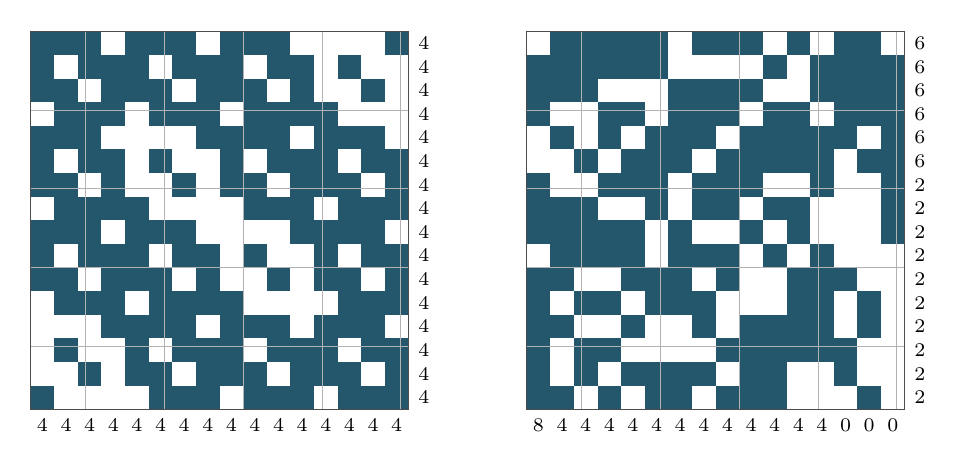
\begin{tikzpicture}[x=3mm,y=3mm,font=\scriptsize]
  \foreach \row [count=\j] in {{1,1,1,0,1,1,1,0,1,1,1,0,0,0,0,1},{1,0,1,1,1,0,1,1,1,0,1,1,0,1,0,0},{1,1,0,1,1,1,0,1,1,1,0,1,0,0,1,0},{0,1,1,1,0,1,1,1,0,1,1,1,1,0,0,0},{1,1,1,0,0,0,0,1,1,1,1,0,1,1,1,0},{1,0,1,1,0,1,0,0,1,0,1,1,1,0,1,1},{1,1,0,1,0,0,1,0,1,1,0,1,1,1,0,1},{0,1,1,1,1,0,0,0,0,1,1,1,0,1,1,1},{1,1,1,0,1,1,1,0,0,0,0,1,1,1,1,0},{1,0,1,1,1,0,1,1,0,1,0,0,1,0,1,1},{1,1,0,1,1,1,0,1,0,0,1,0,1,1,0,1},{0,1,1,1,0,1,1,1,1,0,0,0,0,1,1,1},{0,0,0,1,1,1,1,0,1,1,1,0,1,1,1,0},{0,1,0,0,1,0,1,1,1,0,1,1,1,0,1,1},{0,0,1,0,1,1,0,1,1,1,0,1,1,1,0,1},{1,0,0,0,0,1,1,1,0,1,1,1,0,1,1,1}}
    \foreach \e [count=\k] in \row {\ifnum\e=1 \fill[glowblue] (\k,-\j) rectangle ++(1,1); \fi}
  \draw[black!30,line width=.3pt] (1,-16) grid (17,0); \draw[black!70] (1,-16) rectangle (17,0);
  \foreach \t [count=\j] in {4,4,4,4,4,4,4,4,4,4,4,4,4,4,4,4} \node[right] at (17,-\j+.5) {$\t$};
  \foreach \t [count=\k] in {4,4,4,4,4,4,4,4,4,4,4,4,4,4,4,4} \node[below] at (\k+.5,-16) {$\t$};
  \begin{scope}[shift={(21,0)}]
    \foreach \row [count=\j] in {{0,1,1,1,1,1,0,1,1,1,0,1,0,1,1,0},{1,1,1,1,1,1,0,0,0,0,1,0,1,1,1,1},{1,1,1,0,0,0,1,1,1,1,0,0,1,1,1,1},{1,0,0,1,1,0,1,1,1,0,1,1,0,1,1,1},{0,1,0,1,0,1,1,1,0,1,1,1,1,1,0,1},{0,0,1,0,1,1,1,0,1,1,1,1,1,0,1,1},{1,0,0,1,1,1,0,1,1,1,0,0,1,0,0,1},{1,1,1,0,0,1,0,1,1,0,1,1,0,0,0,1},{1,1,1,1,1,0,1,0,0,1,0,1,0,0,0,1},{0,1,1,1,1,0,1,1,1,0,1,0,1,0,0,0},{1,1,0,0,1,1,1,0,1,0,0,1,1,1,0,0},{1,0,1,1,0,1,1,1,0,0,0,1,1,0,1,0},{1,1,0,0,1,0,0,1,0,1,1,1,1,0,1,0},{1,0,1,1,0,0,0,0,1,1,1,1,1,1,0,0},{1,0,1,0,1,1,1,1,0,1,1,0,0,1,0,0},{1,1,0,1,0,1,1,0,1,1,1,0,0,0,1,0}}
      \foreach \e [count=\k] in \row {\ifnum\e=1 \fill[glowblue] (\k,-\j) rectangle ++(1,1); \fi}
    \draw[black!30,line width=.3pt] (1,-16) grid (17,0); \draw[black!70] (1,-16) rectangle (17,0);
    \foreach \t [count=\j] in {6,6,6,6,6,6,2,2,2,2,2,2,2,2,2,2} \node[right] at (17,-\j+.5) {$\t$};
    \foreach \t [count=\k] in {8,4,4,4,4,4,4,4,4,4,4,4,4,0,0,0} \node[below] at (\k+.5,-16) {$\t$};
  \end{scope}
\end{tikzpicture}
\caption{On the left, the crystalline state of $W_{16}$ coming from the bent function $x_1x_2+x_3x_4$, as the sign matrix $D_aW_{16}D_b$, with the entries $1$ in blue, and with all its row and column sums equal to $4$. On the right, a ground state of $\mathrm{had}_{16.3}$, with the rows and the columns sorted by their sums, which add up to $56$ instead of $64$. The last 3 column sums vanish, so that 3 column spins are free.}\label{fig:crystal}
\end{figure}

The symmetry group of $\mathrm{had}_{16.3}$ is formed by the pairs $(P,Q)$ of signed permutation matrices with $PHQ=H$, and it has order $86016=2^{12}\cdot21$, as computed by the program \texttt{autgroup.py}, by backtracking on the signed images of the columns. Such a pair maps a ground state $(a,b)$ to the ground state $(P^ta,Qb)$, since $\langle HQb,P^ta\rangle=\langle PHQb,a\rangle$, and \texttt{groundstates.py} finds 3 orbits, which are the 3 types above. Thus $\mathrm{had}_{16.3}$ pays for its lack of a crystal both in energy, $-14$ instead of $-16$, and in degeneracy, with many more ground states than the crystals, as is typical for frustrated systems. In the complex array of \cite{cot} the situation is different: every complex Hadamard matrix has ground states of energy exactly $-N$, by the Idel--Wolf theorem, and the difficulty is in their arithmetic \cite{com}. For larger regular matrices, such as the Walsh matrices $W_{4^n}$, the dynamics is simulated in Section~\ref{sec:larger}, and the crystalline states are reached by cooling for $W_{64},W_{256}$, but not for $W_{1024},W_{4096}$, as for the sine model \cite{mp2}. Summarizing, we have:

\begin{samepage}
\begin{thm}\label{thm:ground}
The Ising array of $\mathrm{had}_{16.3}$ has ground state energy $-14$, with $43008$ ground states, forming $3$ orbits of size $14336$ under the symmetry group, with stabilizers of order $6$. In $2$ of these orbits $3$ of the $16$ row spins are free, and in $2$ of them $3$ of the $16$ column spins are free. The ground state entropy per row wire is $\log(43008)/16\simeq0.667$, while for the regular matrices it is $\log(896)/16\simeq0.425$, $\log(384)/16\simeq0.372$ and $\log(128)/16\simeq0.303$.
\end{thm}
\end{samepage}

\begin{proof}
This is the above computation.
\end{proof}

\section{Exact thermodynamics at small N}\label{sec:exact}

Since we know the exact densities of states, we can compute the exact thermodynamics of the small arrays, at all temperatures. We first prove Theorem~\ref{intro:spectrum}.

\medskip

\noindent\textbf{The arrays of order 16.}
The program \texttt{spectrum16.py} compares the 5 densities of states computed by \texttt{glowlaw.py}, in exact integer arithmetic. The density of states $n$ of $\mathrm{had}_{16.3}$ is given by the following numbers of configurations, the values at $-\Omega$ being the same, and the other classes are obtained by adding $c_H$ times the alternating binomial coefficients $(-1)^k\binom{16}{k}$, at the levels $\Omega=64-8k$:

\medskip

\begin{center}
\begin{tabular}{|c|c|c||c|c|c||c|c|c|}
\hline
$\Omega$ & $n(\Omega)$ & $(-1)^k\binom{16}{k}$ & $\Omega$ & $n(\Omega)$ & $(-1)^k\binom{16}{k}$ & $\Omega$ & $n(\Omega)$ & $(-1)^k\binom{16}{k}$\\
\hline
$0$ & $608993280$ & $12870$ & $24$ & $228501504$ & $-4368$ & $48$ & $2580480$ & $120$\\
$4$ & $196933632$ &  & $28$ & $51287040$ &  & $52$ & $161280$ & \\
$8$ & $546846720$ & $-11440$ & $32$ & $94617600$ & $1820$ & $56$ & $43008$ & $-16$\\
$12$ & $162593280$ &  & $36$ & $17052672$ &  & $60$ & $0$ & \\
$16$ & $409903104$ & $8008$ & $40$ & $23623680$ & $-560$ & $64$ & $0$ & $1$\\
$20$ & $105853440$ &  & $44$ & $2989568$ &  &  &  & \\
\hline
\end{tabular}
\end{center}

\medskip

In terms of generating functions, $\sum_\omega n_H(\omega)x^\omega=\sum_\omega n(\omega)x^\omega+c_H(x^4-x^{-4})^{16}$, and with $x=e^{\beta/4}$ this is the formula $Z_H(\beta)=Z(\beta)+c_H(2\sinh\beta)^{16}$ for the partition functions. In particular, each crystalline state comes with the removal of 16 configurations at $\Omega=56$, and the numbers $n_H(56)+16\,n_H(64)=43008$ do not depend on $H$. We can now formulate our main result, already stated as Theorem~\ref{intro:spectrum} in the introduction:

\begin{samepage}
\begin{thm}\label{thm:spectrum}
The densities of states of the $5$ Ising arrays of order $16$ form a $1$-parameter family. With $n$ being the density of states of $\mathrm{had}_{16.3}$, we have
\[
 n_H(64-8k)=n(64-8k)+(-1)^k\binom{16}{k}c_H
\]
for $k=0,\ldots,16$, and $n_H(\omega)=n(\omega)$ for $\omega=4(8)$, where $c_H=2^{14-r}-128$ is the number of crystalline ground states, which are $896,384,128,0,0$ for the classes $\mathrm{had}_{16.0},\ldots,\mathrm{had}_{16.4}$.
\end{thm}
\end{samepage}

\begin{proof}
This is the above computation, for the 5 classes. Conceptually, the difference of 2 densities of states of order 16 is symmetric, it is supported on $8\mathbb Z$ by the computation, and its moments vanish up to order 14, by Theorem~\ref{thm:moments}. On the 17 points $-64,-56,\ldots,64$, the only such vectors are the multiples of $k\to(-1)^k\binom{16}{k}$, because a symmetric vector on these points is determined by its 9 values at $0,8,\ldots,64$, and the 8 conditions on the even moments up to order 14 are independent, by a Vandermonde argument. The formula $c_H=2^{14-r}-128$ then follows from Theorem~\ref{thm:profile}, by comparing 16th moments, since $\sum_k(-1)^k\binom{16}{k}(64-8k)^{16}=8^{16}\,16!$.
\end{proof}

The reduction modulo 16 recovers Theorem~\ref{thm:2adic}, since the alternating binomial row contributes $c_H\sum_k\binom{16}{k}=2^{16}c_H$ to the difference between the numbers of configurations with $\Omega=0(16)$ and $\Omega=8(16)$, and nothing to the residues $4,12$. Figure~\ref{fig:dos} shows the top of the densities of states of $\mathrm{had}_{16.0}$ and $\mathrm{had}_{16.3}$, where the differences are visible.

\begin{figure}[htb!]
\centering
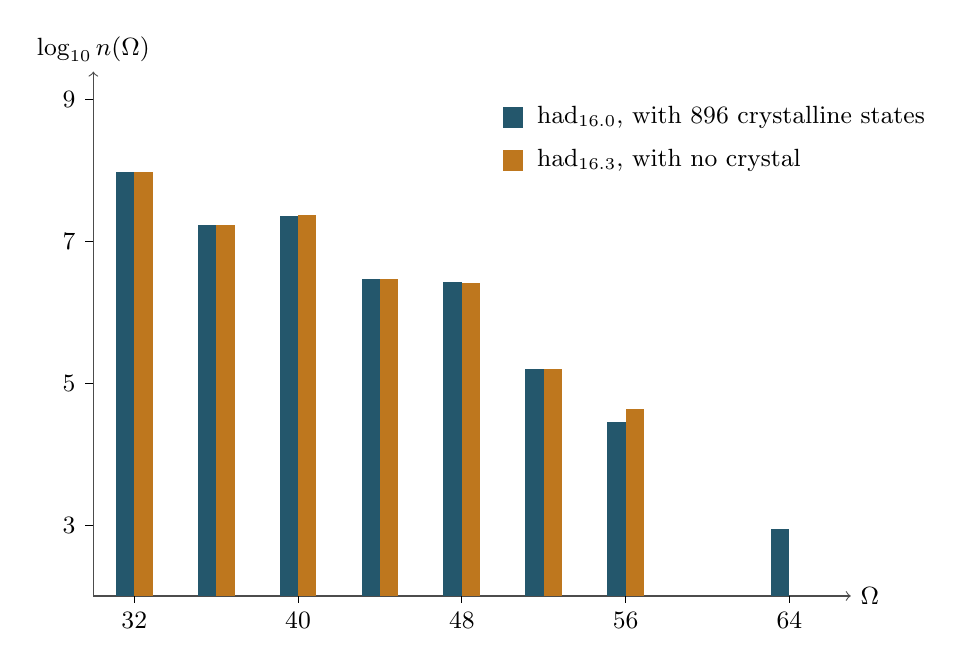
\begin{tikzpicture}[x=2.6mm,y=9mm,font=\small]
  \draw[->,black!70] (30,2)--(67,2) node[right,text=black] {$\Omega$};
  \draw[->,black!70] (30,2)--(30,9.4) node[above,text=black] {$\log_{10}n(\Omega)$};
  \foreach \y in {3,5,7,9} \draw (30,\y)--++(-.4,0) node[left] {$\y$};
  \foreach \x in {32,40,48,56,64} \draw (\x,2)--++(0,-.1) node[below] {$\x$};
  \foreach \x/\v in {32/7.983,36/7.232,40/7.364,44/6.476,48/6.429,52/5.208,56/4.457,64/2.952}
    \fill[glowblue] (\x-.9,2) rectangle (\x,\v);
  \foreach \x/\v in {32/7.976,36/7.232,40/7.373,44/6.476,48/6.412,52/5.208,56/4.634}
    \fill[glowgold] (\x,2) rectangle (\x+.9,\v);
  \fill[glowblue] (50,8.6) rectangle (51,8.9); \node[right] at (51.2,8.75) {$\mathrm{had}_{16.0}$, with 896 crystalline states};
  \fill[glowgold] (50,8.0) rectangle (51,8.3); \node[right] at (51.2,8.15) {$\mathrm{had}_{16.3}$, with no crystal};
\end{tikzpicture}
\caption{The top of the densities of states of $\mathrm{had}_{16.0}$ and $\mathrm{had}_{16.3}$, on a logarithmic scale. The crystalline states at $\Omega=64$ exist only for $\mathrm{had}_{16.0}$, which in return has fewer states at $\Omega=56$. The levels $\Omega=4(8)$ are the same for all classes.}\label{fig:dos}
\end{figure}

\medskip

\noindent\textbf{Energy and specific heat.}
From the exact partition functions, the program \texttt{thermo.py} computes the normalized mean energy $m=E_\beta(\Omega)/N^{3/2}$, the specific heat per row wire $c=\beta^2Var_\beta(\Omega/\sqrt N)/N$, and the entropy per row wire, and \texttt{figures.py} produces the coordinates of the following plots. At high temperature, all the arrays follow the limiting curve of Theorem~\ref{thm:free} very closely, the values of $m$ at $\beta=1/4,1/2,1$ being $0.2365,0.4161,0.6226$ for $\mathrm{had}_{16.0}$, against $0.2361,0.4142,0.6180$ for the limiting curve. At lower temperature, the regular matrices crystallize, while $\mathrm{had}_{16.3}$ stays close to the limiting curve down to $\beta\simeq3$, where it starts freezing towards its ground state value $m=56/64=0.875$.

\begin{figure}[htb!]
\centering
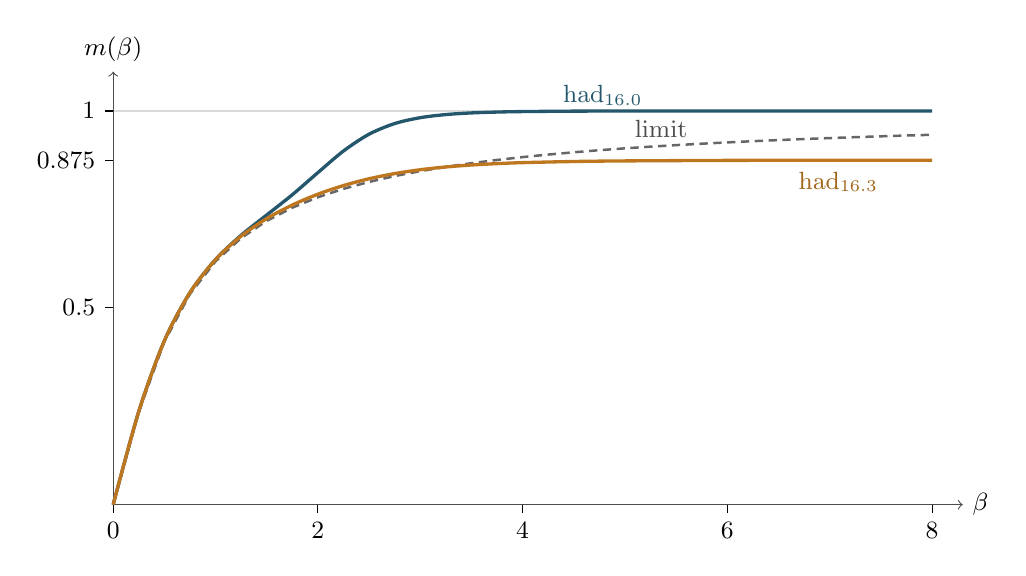
\begin{tikzpicture}[x=13mm,y=50mm,font=\small]
  \draw[black!15] (0,1)--(8,1);
  \draw[->,black!70] (0,0)--(8.3,0) node[right,text=black] {$\beta$};
  \draw[->,black!70] (0,0)--(0,1.1) node[above,text=black] {$m(\beta)$};
  \foreach \x in {0,2,4,6,8} \draw (\x,0)--++(0,-.02) node[below] {$\x$};
  \foreach \y in {0.5,0.875,1} \draw (0,\y)--++(-.08,0) node[left] {$\y$};
  \draw[black!60,densely dashed,line width=.9pt] plot coordinates {(0,0.0000) (0.25,0.2361) (0.5,0.4142) (0.75,0.5352) (1,0.6180) (1.25,0.6770) (1.5,0.7208) (1.75,0.7543) (2,0.7808) (2.25,0.8022) (2.5,0.8198) (2.75,0.8346) (3,0.8471) (3.25,0.8579) (3.5,0.8673) (3.75,0.8755) (4,0.8828) (4.25,0.8892) (4.5,0.8950) (4.75,0.9003) (5,0.9050) (5.25,0.9093) (5.5,0.9132) (5.75,0.9168) (6,0.9201) (6.25,0.9232) (6.5,0.9260) (6.75,0.9287) (7,0.9311) (7.25,0.9334) (7.5,0.9356) (7.75,0.9376) (8,0.9395)};
  \draw[glowblue,line width=1.2pt] plot[smooth] coordinates {(0,0.0000) (0.25,0.2365) (0.5,0.4161) (0.75,0.5385) (1,0.6226) (1.25,0.6842) (1.5,0.7357) (1.75,0.7872) (2,0.8434) (2.25,0.8983) (2.5,0.9410) (2.75,0.9680) (3,0.9829) (3.25,0.9908) (3.5,0.9950) (3.75,0.9972) (4,0.9984) (4.5,0.9995) (5,0.9998) (6,1.0000) (7,1.0000) (8,1.0000)};
  \draw[glowgold,line width=1.2pt] plot[smooth] coordinates {(0,0.0000) (0.25,0.2365) (0.5,0.4161) (0.75,0.5385) (1,0.6223) (1.25,0.6821) (1.5,0.7266) (1.75,0.7611) (2,0.7886) (2.25,0.8105) (2.5,0.8278) (2.75,0.8409) (3,0.8507) (3.25,0.8577) (3.5,0.8627) (3.75,0.8662) (4,0.8687) (4.5,0.8716) (5,0.8731) (6,0.8744) (7,0.8748) (8,0.8749)};
  \node[glowblue,right] at (4.3,1.04) {$\mathrm{had}_{16.0}$};
  \node[glowgold!85!black,right] at (6.6,0.82) {$\mathrm{had}_{16.3}$};
  \node[black!70,right] at (5.0,0.955) {limit};
\end{tikzpicture}
\caption{The normalized energy $m(\beta)$ of the arrays of $\mathrm{had}_{16.0}$, which crystallizes, and of $\mathrm{had}_{16.3}$, which freezes at $0.875$. The dashed line is the limiting curve $(\sqrt{1+4\beta^2}-1)/(2\beta)$.}\label{fig:energy}
\end{figure}

The specific heat, shown in Figure~\ref{fig:heat}, makes the difference even clearer. The 3 regular arrays of order 16 have a sharp maximum, of height about 1, at the temperatures $T\simeq0.451,0.400,0.335$, the more crystalline states the higher the temperature, while $\mathrm{had}_{16.3}$ only has a broad maximum, of height $0.40$, at $T\simeq0.463$, as computed by \texttt{crystal.py}. This is the finite size picture of a crystallization, against a smooth freezing. At low temperature the crystalline term $c_H(2\sinh\beta)^{16}$ of Theorem~\ref{intro:spectrum} dominates the partition function, and the specific heat of the regular arrays then decays like the one of a gapped system, the first excitations being at $\Omega=56$, while for $\mathrm{had}_{16.3}$ the gap is between $56$ and $52$, and its ground states are much more numerous.

\medskip

\noindent\textbf{Crystallization.} These temperatures can be predicted. Per row wire, the crystalline states have free energy $-1-\log(c_H)/(N\beta)$, while the paramagnetic phase has, in the large $N$ limit, the free energy $-(2\log2+\Psi(\beta))/\beta$ of Theorem~\ref{thm:free}. These cross when
\[
 \beta+\frac{\log c_H}{N}=2\log2+\Psi(\beta)
\]
and the program \texttt{crystal.py} finds that at $N=16$ the solutions are $T_c=0.444,0.394,0.339$ for $\mathrm{had}_{16.0},\mathrm{had}_{16.1},\mathrm{had}_{16.2}$, very close to the maxima of the specific heat, and this works even better at $N=36$, as explained in Section~\ref{sec:larger}. For the Walsh matrices, $c_H$ is the number of bent functions, and the table in Section~\ref{sec:ground} gives $T_c=0.551,0.444,0.376,0.328$ at $N=4,16,64,256$. As $N\to\infty$, the limit points of $T_c$ lie between $0.178$, which is the solution when $\log c_H=o(N)$, and $0.295$, coming from the upper bound in \cite{pot}, and finding the limit would require the asymptotics of the number of bent functions. In all cases the crystallization temperature is well above the dynamical glass temperature $T_G\simeq0.14$ of the fully frustrated hypercube \cite{mp3}, so the arrays of regular matrices should behave as the sine model of \cite{mp2}, with a first order transition to the crystal at $T_c$, which is missed when cooling, the system staying in the supercooled paramagnetic phase down to the glass transition.

\begin{figure}[htb!]
\centering
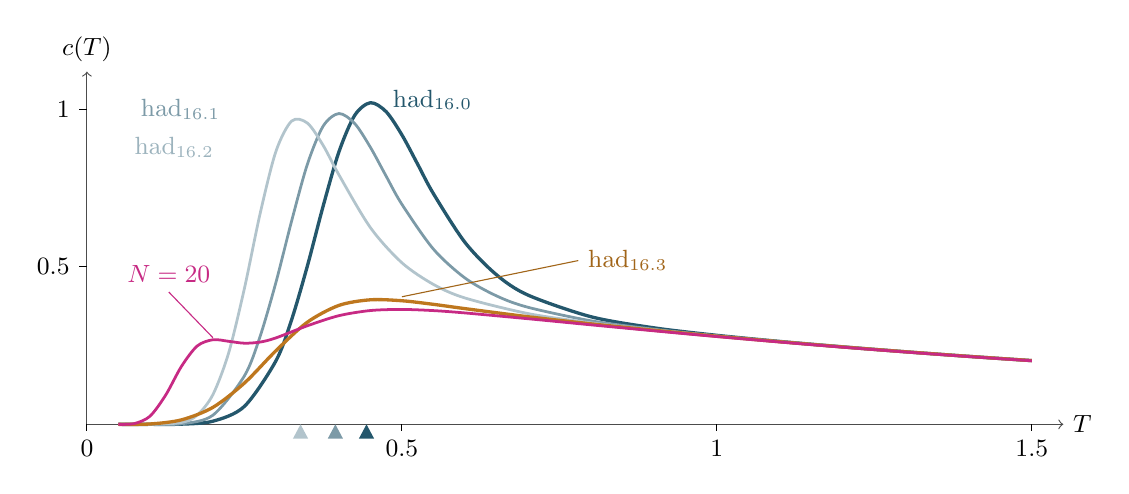
\begin{tikzpicture}[x=80mm,y=40mm,font=\small]
  \draw[->,black!70] (0,0)--(1.55,0) node[right,text=black] {$T$};
  \draw[->,black!70] (0,0)--(0,1.12) node[above,text=black] {$c(T)$};
  \foreach \x in {0,0.5,1,1.5} \draw (\x,0)--++(0,-.02) node[below] {$\x$};
  \foreach \y in {0.5,1} \draw (0,\y)--++(-.012,0) node[left] {$\y$};
  \draw[glowblue,line width=1.2pt] plot[smooth] coordinates {(0.050,0.0000) (0.100,0.0000) (0.150,0.0006) (0.200,0.0100) (0.250,0.0571) (0.300,0.2015) (0.325,0.3326) (0.350,0.5032) (0.375,0.6930) (0.400,0.8649) (0.425,0.9808) (0.450,1.0211) (0.475,0.9926) (0.500,0.9190) (0.525,0.8260) (0.550,0.7325) (0.600,0.5780) (0.650,0.4751) (0.700,0.4105) (0.800,0.3417) (0.900,0.3064) (1.000,0.2826) (1.100,0.2632) (1.200,0.2460) (1.300,0.2303) (1.400,0.2158) (1.500,0.2023)};
  \draw[glowblue!60,line width=1pt] plot[smooth] coordinates {(0.050,0.0000) (0.100,0.0000) (0.150,0.0017) (0.200,0.0291) (0.250,0.1539) (0.275,0.2798) (0.300,0.4505) (0.325,0.6461) (0.350,0.8261) (0.375,0.9469) (0.400,0.9868) (0.425,0.9552) (0.450,0.8796) (0.475,0.7879) (0.500,0.6986) (0.550,0.5564) (0.600,0.4648) (0.650,0.4080) (0.700,0.3717) (0.800,0.3288) (0.900,0.3020) (1.000,0.2810) (1.100,0.2626) (1.200,0.2458) (1.300,0.2302) (1.400,0.2158) (1.500,0.2023)};
  \draw[glowblue!35,line width=1pt] plot[smooth] coordinates {(0.050,0.0000) (0.100,0.0000) (0.150,0.0058) (0.175,0.0291) (0.200,0.0944) (0.225,0.2270) (0.250,0.4316) (0.275,0.6697) (0.300,0.8666) (0.325,0.9630) (0.350,0.9564) (0.375,0.8856) (0.400,0.7923) (0.450,0.6246) (0.500,0.5130) (0.550,0.4443) (0.600,0.4012) (0.700,0.3518) (0.800,0.3223) (0.900,0.2998) (1.000,0.2802) (1.100,0.2623) (1.200,0.2457) (1.300,0.2302) (1.400,0.2157) (1.500,0.2023)};
  \draw[glowgold,line width=1.2pt] plot[smooth] coordinates {(0.050,0.0000) (0.100,0.0011) (0.150,0.0142) (0.200,0.0539) (0.250,0.1311) (0.300,0.2337) (0.350,0.3244) (0.400,0.3776) (0.450,0.3954) (0.500,0.3924) (0.550,0.3810) (0.600,0.3674) (0.700,0.3417) (0.800,0.3191) (0.900,0.2987) (1.000,0.2798) (1.100,0.2621) (1.200,0.2456) (1.300,0.2302) (1.400,0.2157) (1.500,0.2023)};
  \draw[magenta!80!black,line width=1pt] plot[smooth] coordinates {(0.050,0.0000) (0.075,0.0023) (0.100,0.0257) (0.125,0.0929) (0.150,0.1839) (0.175,0.2487) (0.200,0.2686) (0.225,0.2636) (0.250,0.2576) (0.275,0.2612) (0.300,0.2744) (0.350,0.3130) (0.400,0.3450) (0.450,0.3613) (0.500,0.3648) (0.550,0.3611) (0.600,0.3537) (0.700,0.3353) (0.800,0.3159) (0.900,0.2969) (1.000,0.2786) (1.100,0.2613) (1.200,0.2449) (1.300,0.2296) (1.400,0.2152) (1.500,0.2018)};
  \node[glowblue,right] at (0.47,1.03) {$\mathrm{had}_{16.0}$};
  \node[glowblue!60,right] at (0.07,1.0) {$\mathrm{had}_{16.1}$};
  \node[glowblue!45,right] at (0.06,0.88) {$\mathrm{had}_{16.2}$};
  \draw[glowgold!85!black] (0.5,0.405)--(0.78,0.52) node[right] {$\mathrm{had}_{16.3}$};
  \draw[magenta!80!black] (0.2,0.275)--(0.13,0.42) node[above] {$N=20$};
  \foreach \t/\c in {0.4438/glowblue,0.3944/glowblue!60,0.3391/glowblue!35} \fill[\c] (\t,0)--(\t-.012,-.045)--(\t+.012,-.045)--cycle;
\end{tikzpicture}
\caption{The specific heat per row wire of the arrays of order 16 and 20, as a function of the temperature. The 3 regular arrays of order 16 crystallize, near the temperatures $T_c$ marked by triangles, while $\mathrm{had}_{16.3}$ and the arrays of order 20 freeze smoothly.}\label{fig:heat}
\end{figure}

\medskip

\noindent\textbf{The arrays of order 20.}
There are 3 Hadamard matrices of order 20, up to equivalence \cite{ha2}, and \texttt{glowlaw.py} finds that their densities of states coincide, at all the 41 levels $\Omega=-80,-76,\ldots,80$. Thus the 3 arrays are thermodynamically indistinguishable, at all temperatures, although they are inequivalent, their symmetry groups having orders $5760$, $3840$ and $6840$. None of them has a crystalline state, since 20 is not a square, and their ground states, at $\Omega=80$, are $40128$ in number, with $|Hb|$ given by $6$ on 10 rows and $2$ on 10 rows, and with no free spins. Their specific heat has 2 maxima, a shoulder at $T\simeq0.2$, coming from the 40128 ground states and the next level at $\Omega=76$, and a broad maximum at $T\simeq0.5$. In other words, one cannot hear the shape of a Hadamard array of order 20. This coincidence goes far beyond the universality of the moments up to order 14, and it even holds at a finer level: the program \texttt{multisets.py} finds that the 3 matrices have the same distribution of the multisets of numbers $|(Hb)_j|$, with the same 15 multisets, having the same multiplicities. We have no explanation for this, and it would be interesting to find a general mechanism producing inequivalent Hadamard matrices with the same density of states, as for the isospectral graphs. We obtain:

\begin{samepage}
\begin{thm}\label{thm:exact}
The $3$ Ising arrays of order $20$ have the same density of states, and therefore the same thermodynamics at all temperatures. At $N=16$, the specific heat of the $3$ regular arrays has a maximum of height about $1$, at a temperature which increases with the number of crystalline states, and is close to the crystallization temperature $T_c$, while the array of $\mathrm{had}_{16.3}$ has a broad maximum of height about $0.4$.
\end{thm}
\end{samepage}

\begin{proof}
This is the above computation, done in exact integer arithmetic for the densities of states, and in floating point for the thermodynamic functions and for $T_c$.
\end{proof}

\section{Dynamics and larger orders}\label{sec:larger}

In this section we look at larger arrays, first with the Metropolis dynamics, in the spirit of \cite{mp2,mp3}, and then with exact computations at $N=24,28,36$.

\medskip

\noindent\textbf{Dynamics.} The program \texttt{dynamics.py} simulates the Metropolis dynamics of the arrays, with single spin flips, by using the C program \texttt{mc.c}, which keeps the integer local fields $Hb$ and $H^ta$ up to date, so that a flip costs $O(N)$. We use the Walsh matrices $W_{64}$ and $W_{256}$, which have crystalline states, and the Paley matrix of order 252, coming from $q=251$ \cite{pal}, which has none, 252 not being a square. We cool slowly, from $T=1$ down to $T=0.02$, by steps of $0.025$, with $10^4$ sweeps at each temperature, starting from 8 random configurations. For the Walsh matrices we also heat, starting from a crystalline state, built from the bent function $(-1)^{\langle x,y\rangle}$ of Maiorana and McFarland \cite{tok}. The results are shown in Figure~\ref{fig:dynamics}.

\begin{figure}[htb!]
\centering
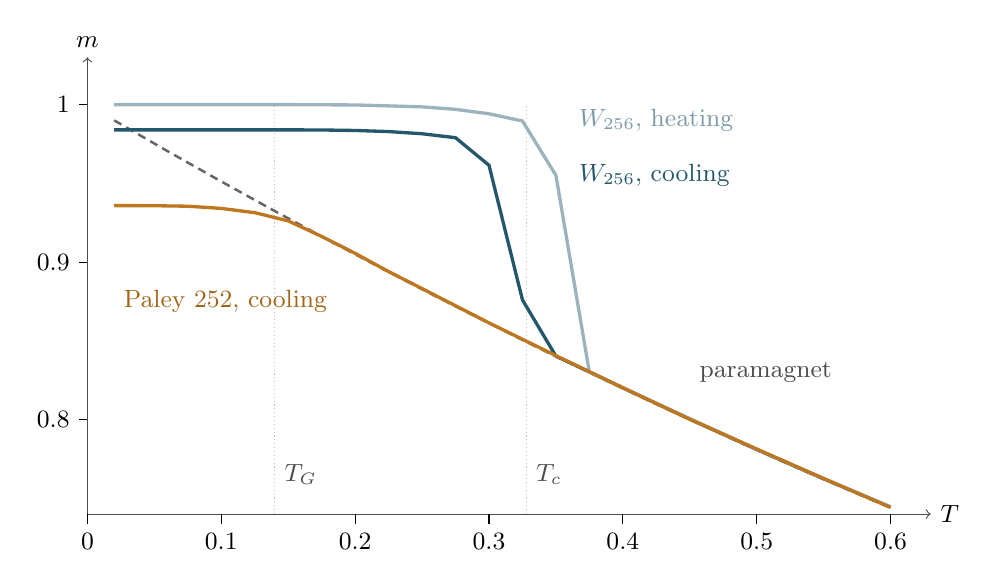
\begin{tikzpicture}[x=170mm,y=200mm,font=\small]
 \begin{scope}[shift={(0,-0.74)}]
  \draw[->,black!70] (0,0.74)--(0.63,0.74) node[right,text=black] {$T$};
  \draw[->,black!70] (0,0.74)--(0,1.03) node[above,text=black] {$m$};
  \foreach \x in {0,0.1,0.2,0.3,0.4,0.5,0.6} \draw (\x,0.74)--++(0,-.006) node[below] {$\x$};
  \foreach \y in {0.8,0.9,1} \draw (0,\y)--++(-.006,0) node[left] {$\y$};
  \draw[black!25,densely dotted] (0.328,0.74)--(0.328,1.0); \node[right,black!70] at (0.328,0.765) {$T_c$};
  \draw[black!25,densely dotted] (0.14,0.74)--(0.14,1.0); \node[right,black!70] at (0.14,0.765) {$T_G$};
  \draw[black!60,densely dashed,line width=.9pt] plot coordinates {(0.020,0.9900) (0.040,0.9802) (0.060,0.9704) (0.080,0.9608) (0.100,0.9512) (0.120,0.9418) (0.140,0.9324) (0.160,0.9232) (0.180,0.9140) (0.200,0.9050) (0.220,0.8960) (0.240,0.8872) (0.260,0.8784) (0.280,0.8698) (0.300,0.8612) (0.320,0.8527) (0.340,0.8443) (0.360,0.8361) (0.380,0.8279) (0.400,0.8198) (0.420,0.8118) (0.440,0.8039) (0.460,0.7961) (0.480,0.7884) (0.500,0.7808) (0.520,0.7732) (0.540,0.7658) (0.560,0.7585) (0.580,0.7512) (0.600,0.7440)};
  \draw[glowblue,line width=1.2pt] plot coordinates {(0.020,0.9840) (0.050,0.9840) (0.100,0.9840) (0.150,0.9840) (0.175,0.9839) (0.200,0.9836) (0.225,0.9829) (0.250,0.9815) (0.275,0.9790) (0.300,0.9615) (0.325,0.8760) (0.350,0.8403) (0.375,0.8303) (0.400,0.8202) (0.450,0.8004) (0.500,0.7810) (0.550,0.7624) (0.600,0.7445)};
  \draw[glowblue!45,line width=1.2pt] plot coordinates {(0.020,1.0000) (0.150,1.0000) (0.200,0.9998) (0.250,0.9986) (0.275,0.9970) (0.300,0.9942) (0.325,0.9896) (0.350,0.9551) (0.375,0.8301) (0.400,0.8202) (0.450,0.8006) (0.500,0.7812) (0.550,0.7626) (0.600,0.7446)};
  \draw[glowgold,line width=1.2pt] plot coordinates {(0.020,0.9359) (0.050,0.9358) (0.075,0.9355) (0.100,0.9341) (0.125,0.9314) (0.150,0.9262) (0.175,0.9163) (0.200,0.9056) (0.225,0.8940) (0.250,0.8832) (0.300,0.8614) (0.350,0.8406) (0.400,0.8202) (0.450,0.8002) (0.500,0.7813) (0.550,0.7626) (0.600,0.7442)};
  \node[glowblue!60,right] at (0.36,0.99) {$W_{256}$, heating};
  \node[glowblue,right] at (0.36,0.955) {$W_{256}$, cooling};
  \node[glowgold!85!black,right] at (0.02,0.875) {Paley 252, cooling};
  \node[black!70,right] at (0.45,0.83) {paramagnet};
 \end{scope}
\end{tikzpicture}
\caption{The normalized energy $m$ of the arrays of $W_{256}$, on cooling from random configurations and on heating from a crystalline state, and of the Paley matrix of order 252, on cooling, averaged over the runs. The dashed line is the paramagnetic curve of Theorem~\ref{thm:free}, and the dotted lines mark the crystallization temperature $T_c$ of Section~\ref{sec:exact}, and the dynamical glass temperature $T_G$ of the hypercube \cite{mp3}.}\label{fig:dynamics}
\end{figure}

At high temperature all the arrays follow the paramagnetic curve of Theorem~\ref{thm:free}, within $0.003$ for $T\geq0.5$. The array of $W_{64}$ crystallizes reversibly, the cooling and heating curves coinciding, with a maximum of the specific heat at $T\simeq0.375$, in agreement with the value $T_c=0.376$ of Section~\ref{sec:exact}. For $W_{256}$ there is hysteresis, as for a first order transition. On cooling, the array stays paramagnetic down to $T=0.35$, and crystallizes around $T\simeq0.32$, while on heating the crystal survives up to $T=0.325$, and melts around $T\simeq0.35$, so that the hysteresis loop contains $T_c=0.328$. On cooling the crystal is not always reached, the energy after a final quench at $T=0$ being $m=0.984$ on average, between $0.973$ and $1$. The Paley array follows the paramagnetic curve down to $T\simeq0.175$, then freezes, with no sharp maximum of the specific heat, and ends at $m=0.936$ on average, between $0.935$ and $0.938$, in agreement with the values $T_G\simeq0.14$ and $m\simeq0.94$ found in \cite{mp3} for the hypercube. Thus a local search finds, for this Paley matrix, an equivalent matrix with excess about $0.936N^{3/2}$, against the lower bound $N^22^{-N}\binom{N}{N/2}\simeq\sqrt{2/\pi}N^{3/2}\simeq0.80N^{3/2}$ of Best \cite{bes}.

This is the scenario of \cite{mp2}, with a crystallization at $T_c$ for the regular matrices, and a glass transition near $T_G$ for all the matrices, with the difference that at $N=256$ the crystal is still found by a slow cooling, $T_c$ being well above $T_G$. As $N\to\infty$, the crystallization temperature of the Walsh arrays decreases, as explained in Section~\ref{sec:exact}, and the nucleation of a crystal should become harder. In order to see this, we have simulated larger arrays on a laptop, with the script \texttt{stipe.py}, using the same program \texttt{mc.c}, for $W_{1024}$, $W_{4096}$, and the Paley matrix of order 1020, from $q=1019$, the results being summarized by \texttt{dynlarge.py}, as follows:

\begin{center}
\begin{tabular}{|l|c|c|c|}
\hline
matrix & on cooling & final $m$ & crystal melts at\\
\hline
$W_{64}$ & crystallizes & $1$ & $T\simeq0.375$, reversibly\\
$W_{256}$ & crystallizes, mostly & $0.973-1$ & $T\simeq0.35-0.375$\\
$W_{1024}$ & partial order at $T\simeq0.2$ & $0.948-0.956$ & $T\simeq0.375-0.4$\\
$W_{4096}$ & glass & $0.936$ & $T\simeq0.4$\\
Paley 252 & glass & $0.935-0.938$ & no crystal\\
Paley 1020 & glass & $0.936$ & no crystal\\
\hline
\end{tabular}
\end{center}

For $W_{1024}$ the cooling, with 4 runs of $10^4$ sweeps per temperature, leaves the paramagnetic curve around $T\simeq0.2$, and ends in a partially ordered state, and this does not change when cooling 10 times slower in the window $0.45\geq T\geq0.1$, the crystal being never reached. For $W_{4096}$ there is no such ordering at all, and the single cooling run ends at $m=0.9362$, close to the values $0.9365,0.9364$ found for the Paley matrix of order 1020, and to those found for the Paley matrix of order 252. On heating, the crystals survive up to $T\simeq0.375$, well above $T_c$, before melting. Thus, as $N$ grows the crystal is missed, as for the sine model \cite{mp2}, and the energy reached by cooling, $m\simeq0.936$, appears to be about the same for all the large arrays, in our finite runs, in agreement with the energy $m\simeq0.94$ found for the hypercube \cite{mp3}. The cooling curves are shown in Figure~\ref{fig:largedyn}.

\begin{figure}[htb!]
\centering
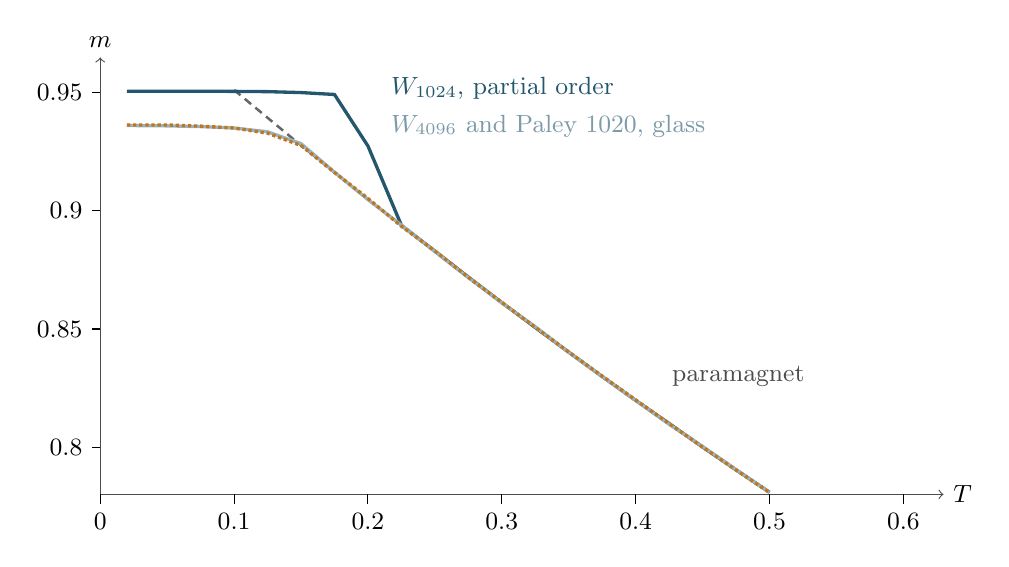
\begin{tikzpicture}[x=170mm,y=300mm,font=\small]
 \begin{scope}[shift={(0,-0.78)}]
  \draw[->,black!70] (0,0.78)--(0.63,0.78) node[right,text=black] {$T$};
  \draw[->,black!70] (0,0.78)--(0,0.965) node[above,text=black] {$m$};
  \foreach \x in {0,0.1,0.2,0.3,0.4,0.5,0.6} \draw (\x,0.78)--++(0,-.004) node[below] {$\x$};
  \foreach \y in {0.8,0.85,0.9,0.95} \draw (0,\y)--++(-.006,0) node[left] {$\y$};
  \draw[black!60,densely dashed,line width=.9pt] plot coordinates {(0.100,0.9512) (0.120,0.9418) (0.140,0.9324) (0.160,0.9232) (0.180,0.9140) (0.200,0.9050) (0.220,0.8960) (0.240,0.8872) (0.260,0.8784) (0.280,0.8698) (0.300,0.8612) (0.320,0.8527) (0.340,0.8443) (0.360,0.8361) (0.380,0.8279) (0.400,0.8198) (0.420,0.8118) (0.440,0.8039) (0.460,0.7961) (0.480,0.7884) (0.500,0.7808)};
  \draw[glowblue,line width=1.2pt] plot coordinates {(0.020,0.9507) (0.030,0.9507) (0.040,0.9507) (0.050,0.9507) (0.075,0.9507) (0.100,0.9506) (0.125,0.9505) (0.150,0.9501) (0.175,0.9493) (0.200,0.9275) (0.225,0.8939) (0.250,0.8830) (0.275,0.8720) (0.300,0.8612) (0.325,0.8507) (0.350,0.8402) (0.375,0.8299) (0.400,0.8198) (0.425,0.8100) (0.450,0.8001) (0.475,0.7904) (0.500,0.7809)};
  \draw[glowblue!45,line width=1.2pt] plot coordinates {(0.020,0.9362) (0.030,0.9361) (0.040,0.9361) (0.050,0.9360) (0.075,0.9357) (0.100,0.9351) (0.125,0.9335) (0.150,0.9285) (0.175,0.9164) (0.200,0.9048) (0.225,0.8940) (0.250,0.8828) (0.275,0.8718) (0.300,0.8611) (0.325,0.8510) (0.350,0.8401) (0.375,0.8299) (0.400,0.8198) (0.425,0.8097) (0.450,0.8003) (0.475,0.7905) (0.500,0.7808)};
  \draw[glowgold,line width=1.2pt,densely dotted] plot coordinates {(0.020,0.9364) (0.030,0.9364) (0.040,0.9364) (0.050,0.9364) (0.075,0.9359) (0.100,0.9351) (0.125,0.9329) (0.150,0.9277) (0.175,0.9163) (0.200,0.9053) (0.225,0.8935) (0.250,0.8831) (0.275,0.8719) (0.300,0.8613) (0.325,0.8507) (0.350,0.8403) (0.375,0.8301) (0.400,0.8200) (0.425,0.8100) (0.450,0.8000) (0.475,0.7903) (0.500,0.7808)};
  \node[glowblue,right] at (0.21,0.952) {$W_{1024}$, partial order};
  \node[glowblue!60,right] at (0.21,0.936) {$W_{4096}$ and Paley 1020, glass};
  \node[black!70,right] at (0.42,0.83) {paramagnet};
 \end{scope}
\end{tikzpicture}
\caption{The cooling curves of the arrays of $W_{1024}$, averaged over 4 runs, of $W_{4096}$, and of the Paley matrix of order 1020, dotted, averaged over 2 runs. The array of $W_{1024}$ jumps to a partially ordered state around $T\simeq0.2$, while the 2 others freeze into a glass, at about the same energy $m\simeq0.936$.}\label{fig:largedyn}
\end{figure}

\noindent\textbf{Exact computations.} Our exact computations of densities of states are summarized in the following table, the cases $N=16,20$ being those of Section~\ref{sec:exact}, and the other ones being explained below. For each order we indicate the number of matrices used, the number of distinct densities of states, the number of parameters of the family that they form, and the ground state energies:

\begin{center}
\begin{tabular}{|c|c|c|c|c|}
\hline
$N$ & matrices & densities of states & parameters & ground states\\
\hline
$16$ & $5$, all & $4$ & $1$ & $m=1$, and $0.875$ for 2 classes\\
$20$ & $3$, all & $1$ & $0$ & $m=0.894$\\
$24$ & $60$, all & $27$ & $2$ & $m=0.953$, and $0.919$ for 4 classes\\
$28$ & $487$, all & $294$ & $4$ & $m=0.945$\\
$32$ & $360$ & $360$ & $\geq8$ & $m=0.928$, except for 5 matrices\\
$36$ & $9$, regular & $9$ & $\geq8$ & $m=1$\\
\hline
\end{tabular}
\end{center}

\medskip

\medskip

\begin{figure}[htb!]
\centering
\begin{tikzpicture}[x=5mm,y=11mm,font=\small]
  \draw[->,black!70] (17,0)--(40,0) node[right,text=black] {$P_4/10^6$};
  \draw[->,black!70] (17,0)--(17,4.6) node[above,text=black] {$n_H(112)/10^3$};
  \foreach \x in {20,25,30,35} \draw (\x,0)--++(0,-.08) node[below] {$\x$};
  \foreach \y/\l in {1/1,2/4,3/9,4/16} \draw (17,\y)--++(-.2,0) node[left] {$\l$};
  \fill[glowblue] (18.653,0.000) circle[radius=1.7pt];
  \fill[glowblue] (23.962,0.000) circle[radius=1.7pt];
  \fill[glowblue] (25.141,0.438) circle[radius=2.2pt];
  \fill[glowblue] (26.321,0.620) circle[radius=2.2pt];
  \fill[glowblue] (26.518,0.716) circle[radius=1.7pt];
  \fill[glowblue] (26.714,0.593) circle[radius=2.2pt];
  \fill[glowblue] (26.714,0.704) circle[radius=1.7pt];
  \fill[glowblue] (27.107,0.566) circle[radius=2.2pt];
  \fill[glowblue] (27.501,0.657) circle[radius=2.7pt];
  \fill[glowblue] (27.501,0.930) circle[radius=3.2pt];
  \fill[glowblue] (27.894,0.912) circle[radius=2.2pt];
  \fill[glowblue] (28.680,0.438) circle[radius=2.2pt];
  \fill[glowblue] (28.680,0.876) circle[radius=3.2pt];
  \fill[glowblue] (28.680,1.159) circle[radius=2.2pt];
  \fill[glowblue] (29.073,1.145) circle[radius=1.7pt];
  \fill[glowblue] (29.467,1.131) circle[radius=1.7pt];
  \fill[glowblue] (30.253,0.800) circle[radius=3.2pt];
  \fill[glowblue] (30.253,1.103) circle[radius=1.7pt];
  \fill[glowblue] (31.039,1.200) circle[radius=3.2pt];
  \fill[glowblue] (31.826,1.497) circle[radius=3.2pt];
  \fill[glowblue] (33.399,1.960) circle[radius=1.7pt];
  \fill[glowblue] (38.117,0.000) circle[radius=2.2pt];
  \fill[glowblue] (38.117,1.315) circle[radius=3.2pt];
  \fill[glowblue] (38.117,1.859) circle[radius=3.2pt];
  \fill[glowblue] (38.117,2.277) circle[radius=2.2pt];
  \fill[glowblue] (38.117,2.939) circle[radius=2.2pt];
  \fill[glowblue] (38.117,4.360) circle[radius=1.7pt];
\end{tikzpicture}
\caption{The 27 densities of states of order 24, as points $(P_4(H),n_H(112))$, the size of each point indicating the number of matrices, from 1 to 4, having this density of states, and the vertical scale being quadratic. The family is affine in these 2 parameters, by Theorem~\ref{thm:order24}.}\label{fig:order24}
\end{figure}

\begin{figure}[htb!]
\centering
\begin{tikzpicture}[x=40mm,y=200mm,font=\small]
  \draw[->,black!70] (2.15,0.1)--(4.65,0.1) node[right,text=black] {ground states};
  \draw[->,black!70] (2.15,0.1)--(2.15,0.42) node[above,text=black] {$T_{max}$};
  \foreach \x/\l in {2.301/200,3/1000,3.699/5000,4.301/20000} \draw (\x,0.1)--++(0,-.004) node[below] {$\l$};
  \foreach \y in {0.2,0.3,0.4} \draw (2.15,\y)--++(-.02,0) node[left] {$\y$};
  \foreach \x/\y/\k in {4.279/0.320/1,3.584/0.254/1,3.350/0.231/4,3.158/0.214/4,2.806/0.190/4,3.715/0.267/2,3.539/0.250/4,3.107/0.210/1,2.885/0.194/4,3.085/0.208/1,2.505/0.172/2,3.128/0.211/2,2.283/0.162/2,3.118/0.210/1,2.920/0.196/2,2.547/0.174/2,2.937/0.197/4,2.584/0.176/2,3.238/0.222/4,2.635/0.179/3,2.695/0.182/1,2.283/0.161/2,2.709/0.183/1,3.937/0.288/2} \fill[glowblue] (\x,\y) circle[radius=0.8pt+0.6pt*\k];
  \foreach \x/\y in {2.505/0.356,2.283/0.364,2.547/0.353,2.584/0.351,2.635/0.345,2.695/0.339,2.283/0.366,2.709/0.337} \draw[glowblue] (\x,\y) circle[radius=1.6pt];
  \foreach \x/\y in {3.848/0.129,3.848/0.385,4.406/0.161,4.406/0.376,4.510/0.171,4.510/0.377} \fill[glowgold] (\x,\y) circle[radius=1.8pt];
\end{tikzpicture}
\caption{The maxima of the specific heat of the arrays of order 24, against their numbers of ground states, on a logarithmic scale. In blue, the 56 matrices with ground states at $\Omega=112$, the size of each point indicating the number of matrices, with the second, smaller maxima in hollow blue, and in gold, the 4 matrices with ground states at $\Omega=108$, which have 2 maxima.}\label{fig:heat24}
\end{figure}

\noindent\textbf{The arrays of order 24.} There are 60 Hadamard matrices of order 24, up to equivalence \cite{ill,ki1,spe}, which are taken from McKay's catalogue \cite{mck}, and converted by \texttt{mckay.py}. The program \texttt{dosall.py} computes their exact densities of states, by using the C program \texttt{dos.c}, which enumerates the $2^{23}$ vectors $b$ with $b_1=1$ in Gray code order, updating $Hb$ in $O(N)$ at each step, and counts them according to the multiset of the numbers $|(Hb)_j|$, the law over $a$ being then obtained by an exact convolution. The program \texttt{structure.py} then analyzes the results, in exact rational arithmetic.

The moments of the 60 densities of states agree up to order 14, and at order 16 their differences are given by the 4-profile, exactly as in Theorem~\ref{thm:moments}, which is a good check. However, the 60 densities of states are far from being independent. There are only 27 of them, the matrices coming in 9 singletons, 10 pairs, 1 triple and 7 quadruples. Part of this is trivial, because the arrays of $H$ and $H^t$ have the same density of states, $\Omega=\langle Hb,a\rangle$ being also equal to $\langle H^ta,b\rangle$. The program \texttt{transpose.py} finds that 2 matrices have the same density of states precisely when they have the same distributions of the multisets of numbers $|(Hb)_j|$ and $|(H^ta)_k|$, up to interchanging them. Among the 55 pairs of matrices having the same density of states, a finer invariant, namely the 4-row profile seen from each row, shows that at least 20 pairs are not related by transposition, so the phenomenon at $N=20$ is present here too. In fact, by \cite{wls} there are 36 classes up to equivalence and transposition, so exactly 24 of these 55 pairs come from transposition, and 31 do not. The program \texttt{permanent.py} computes the permanents, with the C program \texttt{perm.c}, which uses the formula of Glynn, and finds that 2 matrices have the same density of states precisely when they have the same permanent, up to sign, the 27 values of $|per(H)|$ being those found in \cite{wls}. Moreover, the densities of states depend on 2 parameters only. The first one is the number $n_H(112)$ of configurations at $\Omega=112$, where 56 of the 60 matrices have their ground states, the 4 others having them at $\Omega=108$, as in \cite{ckh}, and so having $n_H(112)=0$. A configuration with $\Omega=112$ must have $|Hb|$ given by $4$ on 20 rows and $8$ on 4 rows, because of $\sum_j|(Hb)_j|=112$ and $\sum_j(Hb)_j^2=576$, and because the numbers $(Hb)_j$ are all congruent modulo 4, 2 rows of $H$ differing in $N/2$ positions, so these ground states contribute to the generating function $\sum_\omega n_H(\omega)x^\omega$ by $(x^4+x^{-4})^{20}(x^8+x^{-8})^4$, just as the crystalline states at $N=16$ contribute by $(x^4+x^{-4})^{16}$. As in Theorem~\ref{intro:spectrum}, the correction is the alternating version of this. The second parameter is the quantity $P_4(H)$ of Theorem~\ref{thm:moments}, and the pair $(n_H(112),P_4(H))$ takes 27 values, shown in Figure~\ref{fig:order24}. The temperature of the main maximum of the specific heat is an increasing function of the number of ground states, as shown in Figure~\ref{fig:heat24}, computed by \texttt{pictures.py}, the arrays with fewer ground states having a second, smaller maximum, near $T\simeq0.35$, and with the 4 arrays having their ground states at $\Omega=108$ behaving differently. We obtain:

\begin{samepage}
\begin{thm}\label{thm:order24}
The densities of states of the $60$ Ising arrays of order $24$ form a $2$-parameter family, namely
\[
 n_H=A+n_H(112)V+P_4(H)U
\]
with $A,U$ not depending on $H$, and with $V(\omega)$ being the coefficients of $(x^4-x^{-4})^{20}(x^8-x^{-8})^4$. Thus $2$ arrays of order $24$ have the same density of states precisely when they have the same number of configurations at $\Omega=112$, and the same value of $P_4$, and this happens precisely when they have the same permanent, up to sign.
\end{thm}
\end{samepage}

\begin{proof}
This is the above computation, done in exact arithmetic, the vector $U$ being given in \texttt{structure24.log}, and the permanents in \texttt{permanent24.log}. The generating function of $V$ has a zero of order $24$ at $x=1$, so the ground states are invisible in the moments up to order $22$, which only see $P_4$, and this is indeed what \texttt{structure.py} finds.
\end{proof}

\medskip



\begin{figure}[htb!]
\centering
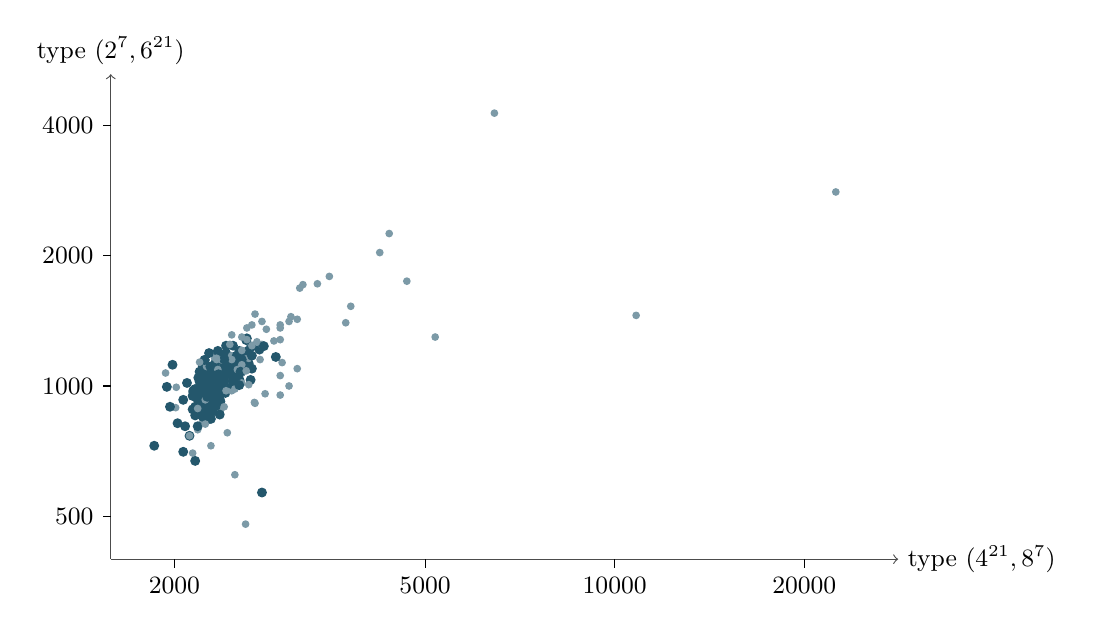
\begin{tikzpicture}[x=80mm,y=55mm,font=\small]
  \draw[->,black!70] (3.2,2.6)--(4.45,2.6) node[right,text=black] {type $(4^{21},8^7)$};
  \draw[->,black!70] (3.2,2.6)--(3.2,3.72) node[above,text=black] {type $(2^7,6^{21})$};
  \foreach \x/\l in {3.301/2000,3.699/5000,4/10000,4.301/20000} \draw (\x,2.6)--++(0,-.02) node[below] {$\l$};
  \foreach \y/\l in {2.699/500,3/1000,3.301/2000,3.602/4000} \draw (3.2,\y)--++(-.012,0) node[left] {$\l$};
  \fill[glowblue!60] (3.400,3.024) circle[radius=1.4pt];
  \fill[glowblue!100] (3.416,3.110) circle[radius=1.8pt];
  \fill[glowblue!60] (3.420,3.089) circle[radius=1.4pt];
  \fill[glowblue!100] (3.394,3.017) circle[radius=1.8pt];
  \fill[glowblue!100] (3.365,3.003) circle[radius=2.6pt];
  \fill[glowblue!100] (3.379,2.988) circle[radius=1.8pt];
  \fill[glowblue!60] (3.397,3.030) circle[radius=1.4pt];
  \fill[glowblue!100] (3.358,3.005) circle[radius=1.8pt];
  \fill[glowblue!100] (3.374,3.043) circle[radius=1.8pt];
  \fill[glowblue!100] (3.367,3.045) circle[radius=1.8pt];
  \fill[glowblue!100] (3.346,3.045) circle[radius=1.8pt];
  \fill[glowblue!100] (3.349,3.060) circle[radius=1.8pt];
  \fill[glowblue!100] (3.370,3.069) circle[radius=1.8pt];
  \fill[glowblue!100] (3.349,3.015) circle[radius=1.8pt];
  \fill[glowblue!100] (3.347,3.027) circle[radius=1.8pt];
  \fill[glowblue!100] (3.385,3.069) circle[radius=1.8pt];
  \fill[glowblue!100] (3.352,2.995) circle[radius=1.8pt];
  \fill[glowblue!60] (3.386,3.049) circle[radius=1.4pt];
  \fill[glowblue!60] (3.414,3.076) circle[radius=1.4pt];
  \fill[glowblue!100] (3.382,3.041) circle[radius=1.8pt];
  \fill[glowblue!60] (3.353,3.020) circle[radius=1.4pt];
  \fill[glowblue!60] (3.374,3.017) circle[radius=1.4pt];
  \fill[glowblue!100] (3.392,3.049) circle[radius=1.8pt];
  \fill[glowblue!100] (3.397,3.020) circle[radius=1.8pt];
  \fill[glowblue!60] (3.374,3.037) circle[radius=1.4pt];
  \fill[glowblue!100] (3.374,2.964) circle[radius=1.8pt];
  \fill[glowblue!60] (3.397,3.052) circle[radius=1.4pt];
  \fill[glowblue!100] (3.394,3.093) circle[radius=1.8pt];
  \fill[glowblue!100] (3.347,2.986) circle[radius=1.8pt];
  \fill[glowblue!100] (3.367,3.057) circle[radius=1.8pt];
  \fill[glowblue!60] (3.374,2.944) circle[radius=1.4pt];
  \fill[glowblue!60] (3.371,2.993) circle[radius=1.4pt];
  \fill[glowblue!100] (3.365,3.020) circle[radius=1.8pt];
  \fill[glowblue!100] (3.397,3.061) circle[radius=1.8pt];
  \fill[glowblue!100] (3.331,2.986) circle[radius=1.8pt];
  \fill[glowblue!100] (3.339,3.019) circle[radius=1.8pt];
  \fill[glowblue!100] (3.339,2.943) circle[radius=1.8pt];
  \fill[glowblue!60] (3.346,2.918) circle[radius=1.4pt];
  \fill[glowblue!60] (3.387,3.054) circle[radius=1.4pt];
  \fill[glowblue!100] (3.347,3.014) circle[radius=1.8pt];
  \fill[glowblue!100] (3.341,3.033) circle[radius=1.8pt];
  \fill[glowblue!100] (3.373,3.019) circle[radius=1.8pt];
  \fill[glowblue!100] (3.393,3.063) circle[radius=1.8pt];
  \fill[glowblue!100] (3.336,2.973) circle[radius=1.8pt];
  \fill[glowblue!100] (3.349,2.950) circle[radius=1.8pt];
  \fill[glowblue!100] (3.362,3.017) circle[radius=1.8pt];
  \fill[glowblue!100] (3.339,2.966) circle[radius=1.8pt];
  \fill[glowblue!100] (3.364,3.029) circle[radius=1.8pt];
  \fill[glowblue!100] (3.330,2.977) circle[radius=1.8pt];
  \fill[glowblue!60] (3.370,2.995) circle[radius=1.4pt];
  \fill[glowblue!100] (3.344,2.960) circle[radius=1.8pt];
  \fill[glowblue!100] (3.379,2.988) circle[radius=1.8pt];
  \fill[glowblue!100] (3.361,2.988) circle[radius=1.8pt];
  \fill[glowblue!100] (3.347,2.993) circle[radius=1.8pt];
  \fill[glowblue!100] (3.386,3.030) circle[radius=1.8pt];
  \fill[glowblue!100] (3.352,2.988) circle[radius=1.8pt];
  \fill[glowblue!100] (3.419,3.052) circle[radius=1.8pt];
  \fill[glowblue!100] (3.379,3.035) circle[radius=1.8pt];
  \fill[glowblue!100] (3.394,3.024) circle[radius=1.8pt];
  \fill[glowblue!100] (3.376,3.048) circle[radius=1.8pt];
  \fill[glowblue!60] (3.385,2.892) circle[radius=1.4pt];
  \fill[glowblue!100] (3.341,2.960) circle[radius=1.8pt];
  \fill[glowblue!60] (3.416,3.134) circle[radius=1.4pt];
  \fill[glowblue!100] (3.383,3.076) circle[radius=1.8pt];
  \fill[glowblue!100] (3.355,2.995) circle[radius=1.8pt];
  \fill[glowblue!60] (3.418,3.063) circle[radius=1.4pt];
  \fill[glowblue!100] (3.370,2.973) circle[radius=1.8pt];
  \fill[glowblue!100] (3.407,3.032) circle[radius=1.8pt];
  \fill[glowblue!100] (3.352,3.025) circle[radius=1.8pt];
  \fill[glowblue!60] (3.472,3.054) circle[radius=1.4pt];
  \fill[glowblue!100] (3.392,3.010) circle[radius=1.8pt];
  \fill[glowblue!100] (3.355,3.019) circle[radius=1.8pt];
  \fill[glowblue!100] (3.401,3.051) circle[radius=1.8pt];
  \fill[glowblue!100] (3.383,3.030) circle[radius=1.8pt];
  \fill[glowblue!100] (3.341,2.982) circle[radius=1.8pt];
  \fill[glowblue!60] (3.303,2.950) circle[radius=1.4pt];
  \fill[glowblue!100] (3.415,3.106) circle[radius=1.8pt];
  \fill[glowblue!60] (3.365,3.064) circle[radius=1.4pt];
  \fill[glowblue!60] (3.424,3.141) circle[radius=1.4pt];
  \fill[glowblue!100] (3.383,3.093) circle[radius=1.8pt];
  \fill[glowblue!100] (3.370,3.081) circle[radius=1.8pt];
  \fill[glowblue!60] (3.380,3.024) circle[radius=1.4pt];
  \fill[glowblue!60] (3.429,3.166) circle[radius=1.4pt];
  \fill[glowblue!60] (3.392,3.118) circle[radius=1.4pt];
  \fill[glowblue!100] (3.331,2.989) circle[radius=1.8pt];
  \fill[glowblue!60] (3.349,2.977) circle[radius=1.4pt];
  \fill[glowblue!60] (3.627,3.308) circle[radius=1.4pt];
  \fill[glowblue!60] (3.368,2.989) circle[radius=1.4pt];
  \fill[glowblue!100] (3.325,2.885) circle[radius=1.8pt];
  \fill[glowblue!100] (3.350,2.986) circle[radius=1.8pt];
  \fill[glowblue!60] (3.386,3.010) circle[radius=1.4pt];
  \fill[glowblue!60] (3.382,3.057) circle[radius=1.4pt];
  \fill[glowblue!100] (3.356,3.024) circle[radius=1.8pt];
  \fill[glowblue!100] (3.341,3.010) circle[radius=1.8pt];
  \fill[glowblue!100] (3.350,3.033) circle[radius=1.8pt];
  \fill[glowblue!60] (3.373,3.041) circle[radius=1.4pt];
  \fill[glowblue!60] (3.459,3.104) circle[radius=1.4pt];
  \fill[glowblue!100] (3.355,2.966) circle[radius=1.8pt];
  \fill[glowblue!100] (3.349,2.980) circle[radius=1.8pt];
  \fill[glowblue!60] (3.352,3.045) circle[radius=1.4pt];
  \fill[glowblue!100] (3.373,3.002) circle[radius=1.8pt];
  \fill[glowblue!100] (3.379,3.032) circle[radius=1.8pt];
  \fill[glowblue!100] (3.394,3.064) circle[radius=1.8pt];
  \fill[glowblue!100] (3.349,3.060) circle[radius=1.8pt];
  \fill[glowblue!100] (3.365,3.049) circle[radius=1.8pt];
  \fill[glowblue!100] (3.422,3.014) circle[radius=1.8pt];
  \fill[glowblue!100] (3.414,3.046) circle[radius=1.8pt];
  \fill[glowblue!100] (3.346,2.958) circle[radius=1.8pt];
  \fill[glowblue!100] (3.365,3.020) circle[radius=1.8pt];
  \fill[glowblue!60] (3.408,3.030) circle[radius=1.4pt];
  \fill[glowblue!100] (3.408,3.061) circle[radius=1.8pt];
  \fill[glowblue!60] (3.419,3.003) circle[radius=1.4pt];
  \fill[glowblue!100] (3.377,3.030) circle[radius=1.8pt];
  \fill[glowblue!100] (3.364,2.973) circle[radius=1.8pt];
  \fill[glowblue!100] (3.404,3.081) circle[radius=1.8pt];
  \fill[glowblue!100] (3.386,3.052) circle[radius=1.8pt];
  \fill[glowblue!100] (3.334,2.993) circle[radius=1.8pt];
  \fill[glowblue!100] (3.330,2.946) circle[radius=1.8pt];
  \fill[glowblue!100] (3.358,3.045) circle[radius=1.8pt];
  \fill[glowblue!100] (3.361,3.009) circle[radius=1.8pt];
  \fill[glowblue!100] (3.361,3.025) circle[radius=1.8pt];
  \fill[glowblue!100] (3.380,3.033) circle[radius=1.8pt];
  \fill[glowblue!100] (3.344,3.000) circle[radius=1.8pt];
  \fill[glowblue!100] (3.331,2.979) circle[radius=1.8pt];
  \fill[glowblue!100] (3.347,2.986) circle[radius=1.8pt];
  \fill[glowblue!100] (3.349,3.022) circle[radius=1.8pt];
  \fill[glowblue!100] (3.352,3.019) circle[radius=1.8pt];
  \fill[glowblue!100] (3.367,3.002) circle[radius=1.8pt];
  \fill[glowblue!100] (3.424,3.091) circle[radius=1.8pt];
  \fill[glowblue!100] (3.424,3.040) circle[radius=1.8pt];
  \fill[glowblue!60] (3.386,3.043) circle[radius=1.4pt];
  \fill[glowblue!100] (3.394,3.014) circle[radius=1.8pt];
  \fill[glowblue!60] (3.359,3.007) circle[radius=1.4pt];
  \fill[glowblue!100] (3.349,2.950) circle[radius=1.8pt];
  \fill[glowblue!100] (3.382,2.991) circle[radius=1.8pt];
  \fill[glowblue!100] (3.408,3.079) circle[radius=1.8pt];
  \fill[glowblue!100] (3.462,3.067) circle[radius=1.8pt];
  \fill[glowblue!100] (3.352,3.022) circle[radius=1.8pt];
  \fill[glowblue!100] (3.350,2.982) circle[radius=1.8pt];
  \fill[glowblue!100] (3.362,3.033) circle[radius=1.8pt];
  \fill[glowblue!60] (3.356,2.979) circle[radius=1.4pt];
  \fill[glowblue!100] (3.418,3.081) circle[radius=1.8pt];
  \fill[glowblue!100] (3.436,3.084) circle[radius=1.8pt];
  \fill[glowblue!60] (3.486,3.160) circle[radius=1.4pt];
  \fill[glowblue!100] (3.382,2.984) circle[radius=1.8pt];
  \fill[glowblue!100] (3.404,3.015) circle[radius=1.8pt];
  \fill[glowblue!100] (3.377,3.020) circle[radius=1.8pt];
  \fill[glowblue!100] (3.397,3.024) circle[radius=1.8pt];
  \fill[glowblue!100] (3.315,2.968) circle[radius=1.8pt];
  \fill[glowblue!100] (3.349,2.973) circle[radius=1.8pt];
  \fill[glowblue!100] (3.306,2.914) circle[radius=1.8pt];
  \fill[glowblue!100] (3.364,3.035) circle[radius=1.8pt];
  \fill[glowblue!100] (3.359,2.986) circle[radius=1.8pt];
  \fill[glowblue!100] (3.368,3.017) circle[radius=1.8pt];
  \fill[glowblue!100] (3.346,3.022) circle[radius=1.8pt];
  \fill[glowblue!100] (3.387,3.054) circle[radius=1.8pt];
  \fill[glowblue!60] (3.547,3.253) circle[radius=1.4pt];
  \fill[glowblue!100] (3.367,3.029) circle[radius=1.8pt];
  \fill[glowblue!60] (3.392,3.070) circle[radius=1.4pt];
  \fill[glowblue!60] (3.416,3.107) circle[radius=1.4pt];
  \fill[glowblue!100] (3.353,2.986) circle[radius=1.8pt];
  \fill[glowblue!100] (3.359,2.993) circle[radius=1.8pt];
  \fill[glowblue!100] (3.362,3.017) circle[radius=1.8pt];
  \fill[glowblue!100] (3.341,2.975) circle[radius=1.8pt];
  \fill[glowblue!60] (3.429,2.960) circle[radius=1.4pt];
  \fill[glowblue!60] (3.670,3.242) circle[radius=1.4pt];
  \fill[glowblue!60] (3.483,3.149) circle[radius=1.4pt];
  \fill[glowblue!100] (3.339,2.958) circle[radius=1.8pt];
  \fill[glowblue!100] (3.367,2.954) circle[radius=1.8pt];
  \fill[glowblue!100] (3.380,3.020) circle[radius=1.8pt];
  \fill[glowblue!100] (3.373,2.969) circle[radius=1.8pt];
  \fill[glowblue!100] (3.353,2.979) circle[radius=1.8pt];
  \fill[glowblue!100] (3.356,2.952) circle[radius=1.8pt];
  \fill[glowblue!100] (3.380,3.027) circle[radius=1.8pt];
  \fill[glowblue!60] (3.330,2.845) circle[radius=1.4pt];
  \fill[glowblue!60] (3.447,3.131) circle[radius=1.4pt];
  \fill[glowblue!100] (3.383,3.058) circle[radius=1.8pt];
  \fill[glowblue!60] (3.379,3.022) circle[radius=1.4pt];
  \fill[glowblue!100] (3.359,3.020) circle[radius=1.8pt];
  \fill[glowblue!100] (3.353,2.952) circle[radius=1.8pt];
  \fill[glowblue!100] (3.368,2.979) circle[radius=1.8pt];
  \fill[glowblue!100] (3.367,3.015) circle[radius=1.8pt];
  \fill[glowblue!100] (3.362,3.014) circle[radius=1.8pt];
  \fill[glowblue!100] (3.370,2.973) circle[radius=1.8pt];
  \fill[glowblue!100] (3.334,2.952) circle[radius=1.8pt];
  \fill[glowblue!100] (3.359,2.997) circle[radius=1.8pt];
  \fill[glowblue!60] (3.408,3.113) circle[radius=1.4pt];
  \fill[glowblue!100] (3.400,3.070) circle[radius=1.8pt];
  \fill[glowblue!100] (3.334,2.979) circle[radius=1.8pt];
  \fill[glowblue!100] (3.380,3.046) circle[radius=1.8pt];
  \fill[glowblue!100] (3.365,2.960) circle[radius=1.8pt];
  \fill[glowblue!100] (3.359,2.924) circle[radius=1.8pt];
  \fill[glowblue!100] (3.334,2.932) circle[radius=1.8pt];
  \fill[glowblue!100] (3.315,2.848) circle[radius=1.8pt];
  \fill[glowblue!60] (3.370,3.038) circle[radius=1.4pt];
  \fill[glowblue!100] (3.393,3.038) circle[radius=1.8pt];
  \fill[glowblue!100] (3.392,2.997) circle[radius=1.8pt];
  \fill[glowblue!60] (3.469,3.134) circle[radius=1.4pt];
  \fill[glowblue!100] (3.368,2.982) circle[radius=1.8pt];
  \fill[glowblue!100] (3.362,2.941) circle[radius=1.8pt];
  \fill[glowblue!100] (3.373,2.934) circle[radius=1.8pt];
  \fill[glowblue!100] (3.385,3.029) circle[radius=1.8pt];
  \fill[glowblue!60] (3.469,3.107) circle[radius=1.4pt];
  \fill[glowblue!100] (3.390,2.995) circle[radius=1.8pt];
  \fill[glowblue!100] (3.380,3.024) circle[radius=1.8pt];
  \fill[glowblue!100] (3.289,2.998) circle[radius=1.8pt];
  \fill[glowblue!100] (3.321,3.007) circle[radius=1.8pt];
  \fill[glowblue!60] (3.368,3.064) circle[radius=1.4pt];
  \fill[glowblue!100] (3.361,3.025) circle[radius=1.8pt];
  \fill[glowblue!100] (3.356,2.986) circle[radius=1.8pt];
  \fill[glowblue!60] (3.338,2.899) circle[radius=1.4pt];
  \fill[glowblue!100] (3.353,3.014) circle[radius=1.8pt];
  \fill[glowblue!60] (3.424,3.093) circle[radius=1.4pt];
  \fill[glowblue!60] (3.408,3.007) circle[radius=1.4pt];
  \fill[glowblue!60] (3.469,2.979) circle[radius=1.4pt];
  \fill[glowblue!60] (3.469,3.141) circle[radius=1.4pt];
  \fill[glowblue!100] (3.440,2.754) circle[radius=1.8pt];
  \fill[glowblue!100] (3.338,2.907) circle[radius=1.8pt];
  \fill[glowblue!100] (3.346,2.930) circle[radius=1.8pt];
  \fill[glowblue!100] (3.347,2.941) circle[radius=2.2pt];
  \fill[glowblue!100] (3.334,2.944) circle[radius=1.8pt];
  \fill[glowblue!100] (3.400,3.040) circle[radius=1.8pt];
  \fill[glowblue!60] (3.437,3.061) circle[radius=1.4pt];
  \fill[glowblue!100] (3.364,2.973) circle[radius=1.8pt];
  \fill[glowblue!100] (3.368,2.989) circle[radius=1.8pt];
  \fill[glowblue!100] (3.373,2.991) circle[radius=1.8pt];
  \fill[glowblue!100] (3.371,3.027) circle[radius=1.8pt];
  \fill[glowblue!60] (3.528,3.236) circle[radius=1.4pt];
  \fill[glowblue!60] (3.432,3.102) circle[radius=1.4pt];
  \fill[glowblue!100] (3.356,3.076) circle[radius=1.8pt];
  \fill[glowblue!60] (3.440,3.096) circle[radius=1.4pt];
  \fill[glowblue!60] (3.440,3.149) circle[radius=1.4pt];
  \fill[glowblue!100] (3.356,2.924) circle[radius=1.8pt];
  \fill[glowblue!100] (3.355,2.973) circle[radius=1.8pt];
  \fill[glowblue!60] (3.408,3.082) circle[radius=1.4pt];
  \fill[glowblue!100] (3.334,2.827) circle[radius=1.8pt];
  \fill[glowblue!60] (3.394,2.993) circle[radius=1.4pt];
  \fill[glowblue!100] (3.298,3.049) circle[radius=1.8pt];
  \fill[glowblue!60] (3.392,2.989) circle[radius=1.4pt];
  \fill[glowblue!100] (3.382,3.051) circle[radius=1.8pt];
  \fill[glowblue!100] (3.386,3.049) circle[radius=1.8pt];
  \fill[glowblue!100] (3.269,2.862) circle[radius=1.8pt];
  \fill[glowblue!100] (3.347,2.928) circle[radius=1.8pt];
  \fill[glowblue!100] (3.294,2.952) circle[radius=1.8pt];
  \fill[glowblue!100] (3.394,3.003) circle[radius=1.8pt];
  \fill[glowblue!60] (3.496,3.154) circle[radius=1.4pt];
  \fill[glowblue!60] (3.397,2.993) circle[radius=1.4pt];
  \fill[glowblue!60] (3.341,3.055) circle[radius=1.4pt];
  \fill[glowblue!60] (3.380,2.952) circle[radius=1.4pt];
  \fill[glowblue!60] (3.483,3.000) circle[radius=1.4pt];
  \fill[glowblue!60] (3.642,3.352) circle[radius=1.4pt];
  \fill[glowblue!60] (3.350,2.968) circle[radius=1.4pt];
  \fill[glowblue!100] (3.318,2.907) circle[radius=1.8pt];
  \fill[glowblue!60] (3.469,3.024) circle[radius=1.4pt];
  \fill[glowblue!60] (3.359,2.862) circle[radius=1.4pt];
  \fill[glowblue!60] (3.445,2.982) circle[radius=1.4pt];
  \fill[glowblue!100] (3.353,2.975) circle[radius=1.8pt];
  \fill[glowblue!100] (3.368,3.017) circle[radius=1.8pt];
  \fill[glowblue!60] (3.287,3.030) circle[radius=1.4pt];
  \fill[glowblue!60] (3.428,2.962) circle[radius=1.4pt];
  \fill[glowblue!60] (3.573,3.146) circle[radius=1.4pt];
  \fill[glowblue!60] (3.715,3.113) circle[radius=1.4pt];
  \fill[glowblue!60] (3.496,3.040) circle[radius=1.4pt];
  \fill[glowblue!60] (3.809,3.630) circle[radius=1.4pt];
  \fill[glowblue!60] (3.581,3.184) circle[radius=1.4pt];
  \fill[glowblue!60] (3.397,2.795) circle[radius=1.4pt];
  \fill[glowblue!60] (4.034,3.163) circle[radius=1.4pt];
  \fill[glowblue!60] (3.414,2.681) circle[radius=1.4pt];
  \fill[glowblue!60] (4.351,3.448) circle[radius=1.4pt];
  \fill[glowblue!60] (3.392,3.061) circle[radius=1.4pt];
  \fill[glowblue!60] (3.325,2.885) circle[radius=1.4pt];
  \fill[glowblue!60] (3.408,3.049) circle[radius=1.4pt];
  \fill[glowblue!100] (3.380,3.010) circle[radius=1.8pt];
  \fill[glowblue!60] (3.350,2.912) circle[radius=1.4pt];
  \fill[glowblue!60] (3.505,3.234) circle[radius=1.4pt];
  \fill[glowblue!60] (3.383,2.989) circle[radius=1.4pt];
  \fill[glowblue!100] (3.394,3.024) circle[radius=1.8pt];
  \fill[glowblue!60] (3.376,3.060) circle[radius=1.4pt];
  \fill[glowblue!100] (3.380,3.061) circle[radius=1.8pt];
  \fill[glowblue!60] (3.304,2.997) circle[radius=1.4pt];
  \fill[glowblue!60] (3.368,3.061) circle[radius=1.4pt];
  \fill[glowblue!100] (3.443,3.092) circle[radius=1.8pt];
  \fill[glowblue!60] (3.401,3.038) circle[radius=1.4pt];
  \fill[glowblue!100] (3.406,3.033) circle[radius=1.8pt];
  \fill[glowblue!100] (3.404,3.002) circle[radius=1.8pt];
  \fill[glowblue!100] (3.424,3.070) circle[radius=1.8pt];
  \fill[glowblue!60] (3.389,3.096) circle[radius=1.4pt];
  \fill[glowblue!100] (3.349,3.005) circle[radius=1.8pt];
  \fill[glowblue!60] (3.415,3.035) circle[radius=1.4pt];
  \fill[glowblue!60] (3.338,2.948) circle[radius=1.4pt];
  \fill[glowblue!60] (3.500,3.226) circle[radius=1.4pt];
  \fill[glowblue!100] (3.347,3.017) circle[radius=1.8pt];
\end{tikzpicture}
\caption{The ground states of the 487 arrays of order 28, all at $\Omega=140$: each point gives the numbers of ground states of the 2 types, on logarithmic scales, with $|Hb|$ given by $4$ on 21 rows and $8$ on 7 rows, horizontally, and by $2$ on 7 rows and $6$ on 21 rows, vertically. The larger points correspond to 2 or more matrices, mostly pairs of matrices having the same density of states.}\label{fig:order28}
\end{figure}

\noindent\textbf{The arrays of order 28.} There are 487 Hadamard matrices of order 28, up to equivalence \cite{ki2,spe}, and we have processed them in the same way, the enumeration by \texttt{dos.c} of the $2^{27}$ vectors $b$ being done on a laptop, with the script \texttt{gaethje.py}, running 4 matrices at a time. Here again the moments agree up to order 14, and their differences at order 16 are given by $P_4$, as in Theorem~\ref{thm:moments}. There are 294 distinct densities of states, the matrices coming in 101 singletons and 193 pairs. For all the 487 matrices, the distributions of the multisets of numbers $|(Hb)_j|$ and $|(H^ta)_k|$ coincide, and 2 matrices have the same density of states precisely when they have the same such distribution. The finer invariant used at $N=24$ is consistent with transposition for 178 of the 193 pairs, and does not decide for the 15 other pairs. In fact, by \cite{wls} there are 294 classes up to equivalence and transposition, and since transposition preserves the density of states, the map from these classes to the 294 densities of states is a bijection, so all the 193 pairs come from transposition. The program \texttt{permanent.py} finds that $|per(H)|$ is a function of the density of states, taking 288 values, as in \cite{wls}, so here the density of states is a finer invariant than the permanent. All the 487 arrays have their ground states at $\Omega=140=5N$, with $|Hb|$ given either by $2$ on 7 rows and $6$ on 21 rows, or by $4$ on 21 rows and $8$ on 7 rows, these being the only possibilities, by the argument used at $N=24$. The densities of states now depend on 4 parameters, $P_4$, seen at order 16, and 3 more parameters, which are invisible in the moments up to order 22, and the program \texttt{structure.py} finds that the numbers $A,B$ of vectors $b$ with $b_1=1$ giving ground states of each type, shown in Figure~\ref{fig:order28}, and the number $C$ of vectors $b$ with $b_1=1$ and $|Hb|$ given by $2$ on 9 rows, $6$ on 18 rows and $10$ on 1 row, suffice, with $n_H(140)=2(A+B)$ and $n_H(136)=2(C+7A)$:


\begin{samepage}
\begin{thm}\label{thm:order28}
The densities of states of the $487$ Ising arrays of order $28$ form a $4$-parameter family, namely $n_H$ is an affine function of $P_4(H)$, and of the numbers of vectors $b$ with $b_1=1$ such that $|Hb|$ is given by $2$ on $7$ rows and $6$ on $21$ rows, by $4$ on $21$ rows and $8$ on $7$ rows, and by $2$ on $9$ rows, $6$ on $18$ rows and $10$ on $1$ row. These $4$ numbers take $294$ values, and $2$ arrays have the same density of states precisely when their matrices are equivalent up to transposition.
\end{thm}
\end{samepage}

\begin{proof}
This follows from the above computation, done in exact arithmetic by \texttt{dosall.py} and \texttt{structure.py}, from the outputs of \texttt{gaethje.py}, with the vectors $b$ of the third type giving the only configurations at $\Omega=136$ with $a_j$ equal to the sign of $(Hb)_j$ for all $j$, and with the last assertion coming from the count of the classes in \cite{wls}.
\end{proof}

\medskip

\begin{figure}[htb!]
\centering
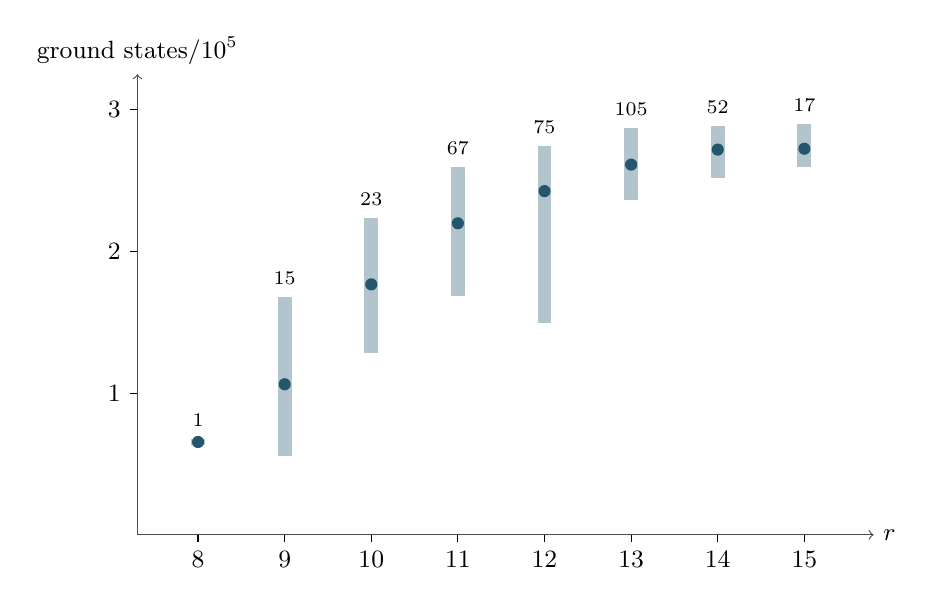
\begin{tikzpicture}[x=11mm,y=18mm,font=\small]
  \draw[->,black!70] (7.3,0)--(15.8,0) node[right,text=black] {$r$};
  \draw[->,black!70] (7.3,0)--(7.3,3.25) node[above,text=black] {ground states$/10^5$};
  \foreach \x in {8,...,15} \draw (\x,0)--++(0,-.05) node[below] {$\x$};
  \foreach \y in {1,2,3} \draw (7.3,\y)--++(-.08,0) node[left] {$\y$};
  \foreach \r/\k/\a/\m/\b in {8/1/0.655/0.655/0.655,9/15/0.573/1.062/1.659,10/23/1.300/1.767/2.217,11/67/1.705/2.198/2.575,12/75/1.516/2.425/2.726,13/105/2.381/2.612/2.847,14/52/2.537/2.718/2.865,15/17/2.616/2.724/2.879} {
    \draw[glowblue!35,line width=5pt] (\r,\a-.02)--(\r,\b+.02);
    \fill[glowblue] (\r,\m) circle[radius=2.2pt];
    \node[above,font=\scriptsize] at (\r,\b+.04) {$\k$};}
\end{tikzpicture}
\caption{The numbers of ground states of the 355 doublings of order 32, all at $\Omega=168$, against the 2-rank $r$: for each value of $r$, the range of these numbers in light blue, their mean in blue, and the number of matrices on top.}\label{fig:order32gs}
\end{figure}

\begin{figure}[htb!]
\centering
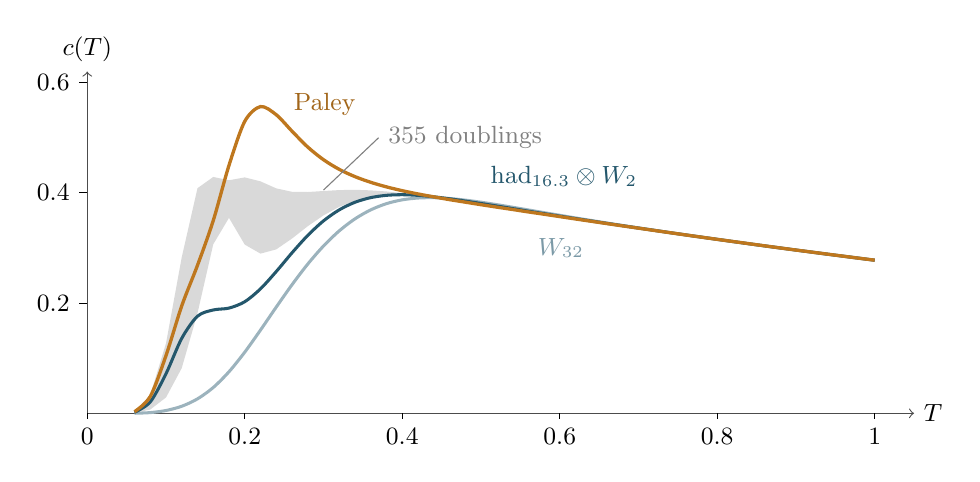
\begin{tikzpicture}[x=100mm,y=70mm,font=\small]
  \draw[->,black!70] (0,0)--(1.05,0) node[right,text=black] {$T$};
  \draw[->,black!70] (0,0)--(0,.62) node[above,text=black] {$c(T)$};
  \foreach \x in {0,0.2,0.4,0.6,0.8,1} \draw (\x,0)--++(0,-.01) node[below] {$\x$};
  \foreach \y in {0.2,0.4,0.6} \draw (0,\y)--++(-.01,0) node[left] {$\y$};
  \fill[black!15] plot coordinates {(0.06,0.0031) (0.08,0.0331) (0.1,0.1269) (0.12,0.2831) (0.14,0.4084) (0.16,0.4288) (0.18,0.4228) (0.2,0.4280) (0.22,0.4208) (0.24,0.4081) (0.26,0.4019) (0.28,0.4015) (0.3,0.4033) (0.32,0.4050) (0.34,0.4055) (0.36,0.4045) (0.38,0.4025) (0.4,0.3995) (0.42,0.3961) (0.44,0.3923) (0.46,0.3885) (0.48,0.3845) (0.5,0.3802) (0.52,0.3757) (0.54,0.3712) (0.56,0.3666) (0.58,0.3621) (0.6,0.3576) (0.62,0.3532) (0.64,0.3488) (0.66,0.3445) (0.68,0.3402) (0.7,0.3360) (0.72,0.3319) (0.74,0.3277) (0.76,0.3236) (0.78,0.3196) (0.8,0.3156) (0.82,0.3117) (0.84,0.3077) (0.86,0.3039) (0.88,0.3000) (0.9,0.2962) (0.92,0.2925) (0.94,0.2887) (0.96,0.2851) (0.98,0.2814) (1,0.2778) (1,0.2778) (0.98,0.2814) (0.96,0.2851) (0.94,0.2887) (0.92,0.2925) (0.9,0.2962) (0.88,0.3000) (0.86,0.3039) (0.84,0.3077) (0.82,0.3116) (0.8,0.3156) (0.78,0.3196) (0.76,0.3236) (0.74,0.3277) (0.72,0.3318) (0.7,0.3359) (0.68,0.3401) (0.66,0.3443) (0.64,0.3485) (0.62,0.3528) (0.6,0.3571) (0.58,0.3614) (0.56,0.3658) (0.54,0.3702) (0.52,0.3745) (0.5,0.3789) (0.48,0.3832) (0.46,0.3875) (0.44,0.3914) (0.42,0.3945) (0.4,0.3959) (0.38,0.3953) (0.36,0.3921) (0.34,0.3855) (0.32,0.3746) (0.3,0.3591) (0.28,0.3394) (0.26,0.3170) (0.24,0.2974) (0.22,0.2897) (0.2,0.3061) (0.18,0.3546) (0.16,0.3066) (0.14,0.1815) (0.12,0.0820) (0.1,0.0287) (0.08,0.0068) (0.06,0.0006)} -- cycle;
  \draw[glowblue!45,line width=1.1pt] plot[smooth] coordinates {(0.06,0.0001) (0.08,0.0013) (0.1,0.0051) (0.12,0.0128) (0.14,0.0262) (0.16,0.0468) (0.18,0.0754) (0.2,0.1109) (0.22,0.1510) (0.24,0.1927) (0.26,0.2332) (0.28,0.2707) (0.3,0.3035) (0.32,0.3310) (0.34,0.3528) (0.36,0.3691) (0.38,0.3804) (0.4,0.3873) (0.42,0.3906) (0.44,0.3912) (0.46,0.3897) (0.48,0.3868) (0.5,0.3830) (0.52,0.3786) (0.54,0.3739) (0.56,0.3690) (0.58,0.3641) (0.6,0.3593) (0.62,0.3545) (0.64,0.3499) (0.66,0.3453) (0.68,0.3408) (0.7,0.3365) (0.72,0.3322) (0.74,0.3279) (0.76,0.3238) (0.78,0.3197) (0.8,0.3157) (0.82,0.3117) (0.84,0.3077) (0.86,0.3038) (0.88,0.3000) (0.9,0.2962) (0.92,0.2924) (0.94,0.2887) (0.96,0.2850) (0.98,0.2814) (1,0.2778)};
  \draw[glowblue,line width=1.1pt] plot[smooth] coordinates {(0.06,0.0019) (0.08,0.0206) (0.1,0.0718) (0.12,0.1360) (0.14,0.1762) (0.16,0.1875) (0.18,0.1909) (0.2,0.2024) (0.22,0.2258) (0.24,0.2572) (0.26,0.2911) (0.28,0.3227) (0.3,0.3491) (0.32,0.3691) (0.34,0.3829) (0.36,0.3913) (0.38,0.3955) (0.4,0.3966) (0.42,0.3954) (0.44,0.3928) (0.46,0.3892) (0.48,0.3851) (0.5,0.3807) (0.52,0.3761) (0.54,0.3715) (0.56,0.3668) (0.58,0.3623) (0.6,0.3577) (0.62,0.3533) (0.64,0.3489) (0.66,0.3445) (0.68,0.3403) (0.7,0.3360) (0.72,0.3319) (0.74,0.3277) (0.76,0.3236) (0.78,0.3196) (0.8,0.3156) (0.82,0.3116) (0.84,0.3077) (0.86,0.3038) (0.88,0.3000) (0.9,0.2962) (0.92,0.2925) (0.94,0.2887) (0.96,0.2851) (0.98,0.2814) (1,0.2778)};
  \draw[glowgold,line width=1.2pt] plot[smooth] coordinates {(0.06,0.0029) (0.08,0.0305) (0.1,0.1047) (0.12,0.1949) (0.14,0.2685) (0.16,0.3496) (0.18,0.4498) (0.2,0.5296) (0.22,0.5565) (0.24,0.5417) (0.26,0.5119) (0.28,0.4831) (0.3,0.4601) (0.32,0.4426) (0.34,0.4294) (0.36,0.4191) (0.38,0.4108) (0.4,0.4039) (0.42,0.3980) (0.44,0.3927) (0.46,0.3877) (0.48,0.3831) (0.5,0.3785) (0.52,0.3741) (0.54,0.3698) (0.56,0.3654) (0.58,0.3612) (0.6,0.3569) (0.62,0.3526) (0.64,0.3484) (0.66,0.3442) (0.68,0.3400) (0.7,0.3359) (0.72,0.3318) (0.74,0.3277) (0.76,0.3236) (0.78,0.3196) (0.8,0.3156) (0.82,0.3117) (0.84,0.3078) (0.86,0.3039) (0.88,0.3000) (0.9,0.2962) (0.92,0.2925) (0.94,0.2888) (0.96,0.2851) (0.98,0.2814) (1,0.2778)};
  \node[glowgold!85!black,right] at (0.25,0.56) {Paley};
  \draw[black!50] (0.3,0.405)--(0.37,0.5) node[right] {355 doublings};
  \node[glowblue,right] at (0.5,0.43) {$\mathrm{had}_{16.3}\otimes W_2$};
  \node[glowblue!60,right] at (0.56,0.3) {$W_{32}$};
\end{tikzpicture}
\caption{The specific heat of the arrays of order 32: the Paley matrix, with ground states at $\Omega=172$, in gold, the region covered by the curves of the 355 doublings, with ground states at $\Omega=168$, in gray, and $\mathrm{had}_{16.3}\otimes W_2$ and $W_{32}$, with ground states at $\Omega=164$ and $160$, in blue.}\label{fig:order32}
\end{figure}

\noindent\textbf{The arrays of order 32.} There are 13710027 Hadamard matrices of order 32, up to equivalence \cite{kta}, and we have used 360 of them, made by \texttt{make32.py}: the Walsh matrix $W_{32}$, the Kronecker products $\mathrm{had}_{16.k}\otimes W_2$ with $k=1,2,3$, the Paley matrix from $q=31$, and 355 doublings $\begin{pmatrix}A&B\\A&-B\end{pmatrix}$, with $A,B$ of order 16, these matrices being kept only when the pair formed by the 4-profiles of $H$ and $H^t$ is new, so that they are inequivalent. Their exact densities of states were computed on 2 laptops, with the scripts \texttt{golovkin.py} and \texttt{valentina.py}, each running \texttt{dos.c} on 180 matrices, in about 1 hour. The 360 densities of states are distinct, the moments agree up to order 14, and the differences of the moments of order 16 to 22 are all proportional to those of $P_4$, as found by \texttt{dosall.py} and \texttt{structure.py}. The densities of states lie in an affine space of dimension 8. For 2 distinct densities of states, the order of the first differing moment is also the order of vanishing at $y=1$ of the difference of their generating functions $F_H(y)=\sum_\omega n_H(\omega)y^{\omega/4}$, and \texttt{structure.py} computes it for all the pairs, at all the orders, with the following results:

\medskip

\begin{center}
\begin{tabular}{|c|c|c|c|c|c|}
\hline
$N$ & pairs & order 16 & order 24 & order 28 & order 32\\
\hline
$24$ & $351$ & $330$ & $21$ & $0$ & $0$\\
$28$ & $43071$ & $42159$ & $911$ & $1$ & $0$\\
$32$ & $64620$ & $64116$ & $494$ & $9$ & $1$\\
$36$ & $36$ & $36$ & $0$ & $0$ & $0$\\
\hline
\end{tabular}
\end{center}

\medskip

\noindent For instance the pair at order 28 for $N=28$ has $\Delta F=16(y-y^{-1})^{28}(y+y^{-1})^7$, and this difference of densities of states, computed by \texttt{pictures.py}, is shown in Figure~\ref{fig:pair28}.

\begin{figure}[htb!]
\centering
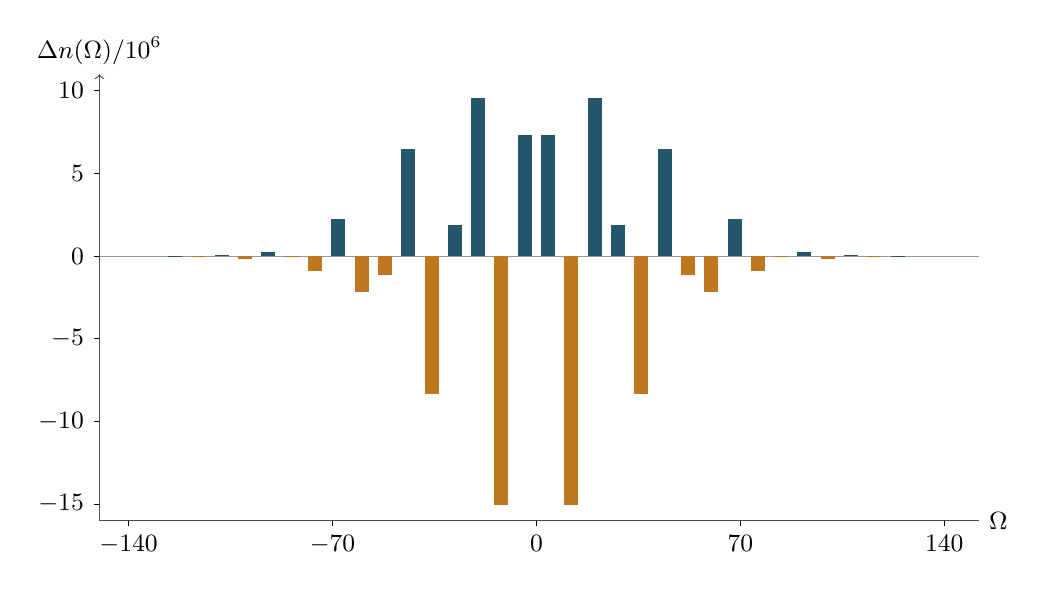
\begin{tikzpicture}[x=.37mm,y=2.1mm,font=\small]
  \draw[black!40] (-150,0)--(152,0);
  \node[right] at (152,-16) {$\Omega$};
  \draw[->,black!70] (-150,-16)--(-150,11) node[above,text=black] {$\Delta n(\Omega)/10^6$};
  \draw[black!70] (-150,-16)--(152,-16);
  \foreach \x in {-140,-70,0,70,140} \draw (\x,-16)--++(0,-.3) node[below] {$\x$};
  \foreach \y in {-15,-10,-5,0,5,10} \draw (-150,\y)--++(-2,0) node[left] {$\y$};
  \foreach \x/\v in {-124/0.003,-108/0.073,-92/0.268,-68/2.216,-44/6.465,-28/1.899,-20/9.583,-4/7.342,4/7.342,20/9.583,28/1.899,44/6.465,68/2.216,92/0.268,108/0.073,124/0.003} \fill[glowblue] (\x-2.4,0) rectangle (\x+2.4,\v);
  \foreach \x/\v in {-116/-0.019,-100/-0.184,-84/-0.017,-76/-0.928,-60/-2.149,-52/-1.136,-36/-8.346,-12/-15.070,12/-15.070,36/-8.346,52/-1.136,60/-2.149,76/-0.928,84/-0.017,100/-0.184,116/-0.019} \fill[glowgold] (\x-2.4,0) rectangle (\x+2.4,\v);
\end{tikzpicture}
\caption{The difference of the densities of states of 2 arrays of order 28 whose moments coincide up to order 26, in units of $10^6$ configurations. It is supported by the levels $\Omega=4(8)$, and given by the coefficients of $16(y-y^{-1})^{28}(y+y^{-1})^7$, with $y$ standing for $x^4$.}\label{fig:pair28}
\end{figure} The ground states are at $\Omega=168=0.928N^{3/2}$ for the 355 doublings, with between $57344$ and $287872$ of them, at $\Omega=164$ for the 3 Kronecker products, and at $\Omega=160$ for $W_{32}$, with $351723520$ of them, while the Paley matrix has its ground states lower, at $\Omega=172$, and only $5952$ of them. For the doublings, the number of ground states tends to increase with the 2-rank $r$, as shown in Figure~\ref{fig:order32gs}, computed by \texttt{pictures.py}, while at $N=16$ the number $2^{14-r}-128$ of crystalline states decreases with $r$.

The specific heat, computed by \texttt{pictures.py} and shown in Figure~\ref{fig:order32}, reflects this distribution of the ground states:

The Paley array has a maximum of height $0.557$ at $T\simeq0.22$, the doublings have maxima of height about $0.42$, at $T\simeq0.15$--$0.20$, and $W_{32}$ and the Kronecker products, which have many more ground states, at a higher energy, only have broad maxima, of height $0.39$, at $T\simeq0.40$--$0.44$. Summarizing, we have:

\begin{samepage}
\begin{thm}\label{thm:order32}
The densities of states of the $360$ Ising arrays of order $32$ above are distinct, and lie in an affine space of dimension $8$. Their moments coincide up to order $14$, and their differences at orders $16$ to $22$ are proportional to those of $P_4$. Their ground states are at $\Omega=168$, except for $W_{32}$, the $3$ Kronecker products and the Paley matrix, where they are at $\Omega=160,164,172$.
\end{thm}
\end{samepage}

\begin{proof}
This follows from the above computation, done in exact arithmetic by \texttt{dosall.py} and \texttt{structure.py}, from the outputs of \texttt{golovkin.py} and \texttt{valentina.py}.
\end{proof}

\medskip

\begin{figure}[htb!]
\centering
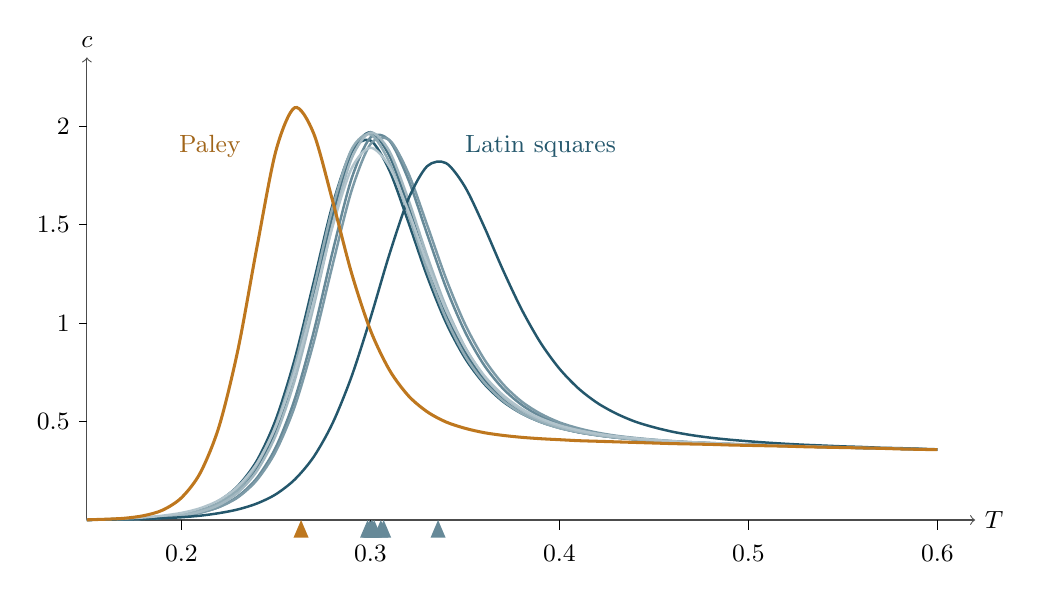
\begin{tikzpicture}[x=240mm,y=25mm,font=\small]
  \draw[->,black!70] (0.15,0)--(0.62,0) node[right,text=black] {$T$};
  \draw[->,black!70] (0.15,0)--(0.15,2.35) node[above,text=black] {$c$};
  \foreach \x in {0.2,0.3,0.4,0.5,0.6} \draw (\x,0)--++(0,-.05) node[below=2pt] {$\x$};
  \foreach \y in {0.5,1,1.5,2} \draw (0.15,\y)--++(-.004,0) node[left] {$\y$};
  \draw[glowblue,line width=.9pt] plot[smooth] coordinates {(0.15,0.002) (0.16,0.003) (0.17,0.006) (0.18,0.010) (0.19,0.018) (0.20,0.031) (0.21,0.056) (0.22,0.098) (0.23,0.174) (0.24,0.303) (0.25,0.512) (0.26,0.819) (0.27,1.209) (0.28,1.602) (0.29,1.873) (0.30,1.928) (0.31,1.777) (0.32,1.515) (0.33,1.239) (0.34,1.003) (0.35,0.823) (0.36,0.694) (0.37,0.603) (0.38,0.541) (0.39,0.498) (0.40,0.468) (0.41,0.446) (0.42,0.431) (0.43,0.419) (0.44,0.410) (0.45,0.403) (0.46,0.398) (0.47,0.393) (0.48,0.389) (0.49,0.385) (0.50,0.382) (0.51,0.379) (0.52,0.376) (0.53,0.374) (0.54,0.371) (0.55,0.369) (0.56,0.366) (0.57,0.364) (0.58,0.362) (0.59,0.360) (0.60,0.357)};
  \draw[glowblue!85,line width=.9pt] plot[smooth] coordinates {(0.15,0.001) (0.16,0.002) (0.17,0.004) (0.18,0.007) (0.19,0.013) (0.20,0.024) (0.21,0.044) (0.22,0.081) (0.23,0.147) (0.24,0.263) (0.25,0.455) (0.26,0.747) (0.27,1.133) (0.28,1.547) (0.29,1.865) (0.30,1.970) (0.31,1.851) (0.32,1.594) (0.33,1.305) (0.34,1.052) (0.35,0.856) (0.36,0.715) (0.37,0.616) (0.38,0.548) (0.39,0.502) (0.40,0.470) (0.41,0.447) (0.42,0.431) (0.43,0.419) (0.44,0.410) (0.45,0.403) (0.46,0.397) (0.47,0.393) (0.48,0.389) (0.49,0.385) (0.50,0.382) (0.51,0.379) (0.52,0.376) (0.53,0.374) (0.54,0.371) (0.55,0.369) (0.56,0.366) (0.57,0.364) (0.58,0.362) (0.59,0.359) (0.60,0.357)};
  \draw[glowblue!70,line width=.9pt] plot[smooth] coordinates {(0.15,0.001) (0.16,0.002) (0.17,0.003) (0.18,0.006) (0.19,0.012) (0.20,0.021) (0.21,0.038) (0.22,0.067) (0.23,0.121) (0.24,0.214) (0.25,0.370) (0.26,0.615) (0.27,0.957) (0.28,1.363) (0.29,1.733) (0.30,1.943) (0.31,1.928) (0.32,1.731) (0.33,1.453) (0.34,1.181) (0.35,0.957) (0.36,0.789) (0.37,0.669) (0.38,0.585) (0.39,0.527) (0.40,0.487) (0.41,0.459) (0.42,0.439) (0.43,0.425) (0.44,0.414) (0.45,0.406) (0.46,0.399) (0.47,0.394) (0.48,0.390) (0.49,0.386) (0.50,0.382) (0.51,0.379) (0.52,0.377) (0.53,0.374) (0.54,0.371) (0.55,0.369) (0.56,0.366) (0.57,0.364) (0.58,0.362) (0.59,0.360) (0.60,0.357)};
  \draw[glowblue!60,line width=.9pt] plot[smooth] coordinates {(0.15,0.001) (0.16,0.002) (0.17,0.004) (0.18,0.007) (0.19,0.012) (0.20,0.021) (0.21,0.037) (0.22,0.066) (0.23,0.116) (0.24,0.204) (0.25,0.350) (0.26,0.578) (0.27,0.903) (0.28,1.296) (0.29,1.672) (0.30,1.909) (0.31,1.931) (0.32,1.763) (0.33,1.499) (0.34,1.227) (0.35,0.996) (0.36,0.820) (0.37,0.692) (0.38,0.602) (0.39,0.540) (0.40,0.496) (0.41,0.466) (0.42,0.444) (0.43,0.428) (0.44,0.417) (0.45,0.408) (0.46,0.401) (0.47,0.395) (0.48,0.391) (0.49,0.387) (0.50,0.383) (0.51,0.380) (0.52,0.377) (0.53,0.374) (0.54,0.371) (0.55,0.369) (0.56,0.367) (0.57,0.364) (0.58,0.362) (0.59,0.360) (0.60,0.357)};
  \draw[glowblue!50,line width=.9pt] plot[smooth] coordinates {(0.15,0.001) (0.16,0.002) (0.17,0.004) (0.18,0.007) (0.19,0.014) (0.20,0.026) (0.21,0.047) (0.22,0.087) (0.23,0.157) (0.24,0.281) (0.25,0.483) (0.26,0.785) (0.27,1.178) (0.28,1.587) (0.29,1.882) (0.30,1.959) (0.31,1.818) (0.32,1.553) (0.33,1.268) (0.34,1.023) (0.35,0.835) (0.36,0.701) (0.37,0.607) (0.38,0.542) (0.39,0.498) (0.40,0.467) (0.41,0.446) (0.42,0.430) (0.43,0.419) (0.44,0.410) (0.45,0.403) (0.46,0.397) (0.47,0.393) (0.48,0.389) (0.49,0.385) (0.50,0.382) (0.51,0.379) (0.52,0.376) (0.53,0.374) (0.54,0.371) (0.55,0.369) (0.56,0.366) (0.57,0.364) (0.58,0.362) (0.59,0.360) (0.60,0.357)};
  \draw[glowblue!42,line width=.9pt] plot[smooth] coordinates {(0.15,0.001) (0.16,0.002) (0.17,0.004) (0.18,0.007) (0.19,0.013) (0.20,0.023) (0.21,0.042) (0.22,0.077) (0.23,0.140) (0.24,0.250) (0.25,0.432) (0.26,0.711) (0.27,1.087) (0.28,1.501) (0.29,1.835) (0.30,1.968) (0.31,1.874) (0.32,1.630) (0.33,1.342) (0.34,1.083) (0.35,0.880) (0.36,0.732) (0.37,0.628) (0.38,0.557) (0.39,0.508) (0.40,0.474) (0.41,0.450) (0.42,0.433) (0.43,0.420) (0.44,0.411) (0.45,0.404) (0.46,0.398) (0.47,0.393) (0.48,0.389) (0.49,0.385) (0.50,0.382) (0.51,0.379) (0.52,0.376) (0.53,0.374) (0.54,0.371) (0.55,0.369) (0.56,0.366) (0.57,0.364) (0.58,0.362) (0.59,0.359) (0.60,0.357)};
  \draw[glowblue,line width=.9pt] plot[smooth] coordinates {(0.15,0.001) (0.16,0.002) (0.17,0.003) (0.18,0.005) (0.19,0.009) (0.20,0.014) (0.21,0.022) (0.22,0.035) (0.23,0.054) (0.24,0.084) (0.25,0.131) (0.26,0.206) (0.27,0.321) (0.28,0.492) (0.29,0.728) (0.30,1.025) (0.31,1.348) (0.32,1.629) (0.33,1.797) (0.34,1.813) (0.35,1.693) (0.36,1.494) (0.37,1.273) (0.38,1.070) (0.39,0.901) (0.40,0.769) (0.41,0.669) (0.42,0.595) (0.43,0.541) (0.44,0.500) (0.45,0.471) (0.46,0.448) (0.47,0.431) (0.48,0.418) (0.49,0.408) (0.50,0.400) (0.51,0.393) (0.52,0.387) (0.53,0.382) (0.54,0.378) (0.55,0.374) (0.56,0.371) (0.57,0.367) (0.58,0.365) (0.59,0.362) (0.60,0.359)};
  \draw[glowblue!35,line width=.9pt] plot[smooth] coordinates {(0.15,0.002) (0.16,0.004) (0.17,0.008) (0.18,0.013) (0.19,0.022) (0.20,0.036) (0.21,0.060) (0.22,0.101) (0.23,0.171) (0.24,0.289) (0.25,0.477) (0.26,0.754) (0.27,1.112) (0.28,1.492) (0.29,1.785) (0.30,1.891) (0.31,1.796) (0.32,1.570) (0.33,1.306) (0.34,1.067) (0.35,0.877) (0.36,0.736) (0.37,0.636) (0.38,0.565) (0.39,0.516) (0.40,0.481) (0.41,0.456) (0.42,0.438) (0.43,0.425) (0.44,0.415) (0.45,0.407) (0.46,0.400) (0.47,0.395) (0.48,0.391) (0.49,0.387) (0.50,0.383) (0.51,0.380) (0.52,0.377) (0.53,0.374) (0.54,0.372) (0.55,0.369) (0.56,0.367) (0.57,0.364) (0.58,0.362) (0.59,0.360) (0.60,0.357)};
  \draw[glowgold,line width=1.1pt] plot[smooth] coordinates {(0.15,0.001) (0.16,0.004) (0.17,0.009) (0.18,0.022) (0.19,0.050) (0.20,0.113) (0.21,0.240) (0.22,0.478) (0.23,0.869) (0.24,1.389) (0.25,1.876) (0.26,2.095) (0.27,1.963) (0.28,1.621) (0.29,1.255) (0.30,0.964) (0.31,0.763) (0.32,0.632) (0.33,0.550) (0.34,0.498) (0.35,0.466) (0.36,0.444) (0.37,0.430) (0.38,0.420) (0.39,0.413) (0.40,0.408) (0.41,0.403) (0.42,0.400) (0.43,0.397) (0.44,0.394) (0.45,0.391) (0.46,0.388) (0.47,0.386) (0.48,0.384) (0.49,0.381) (0.50,0.379) (0.51,0.377) (0.52,0.375) (0.53,0.372) (0.54,0.370) (0.55,0.368) (0.56,0.366) (0.57,0.364) (0.58,0.361) (0.59,0.359) (0.60,0.357)};
  \fill[glowblue!70] (0.2985,0)--(0.2945,-.09)--(0.3025,-.09)--cycle;
  \fill[glowblue!70] (0.3009,0)--(0.2969,-.09)--(0.3049,-.09)--cycle;
  \fill[glowblue!70] (0.3055,0)--(0.3015,-.09)--(0.3095,-.09)--cycle;
  \fill[glowblue!70] (0.307,0)--(0.303,-.09)--(0.311,-.09)--cycle;
  \fill[glowblue!70] (0.2997,0)--(0.2957,-.09)--(0.3037,-.09)--cycle;
  \fill[glowblue!70] (0.302,0)--(0.298,-.09)--(0.306,-.09)--cycle;
  \fill[glowblue!70] (0.3358,0)--(0.3318,-.09)--(0.3398,-.09)--cycle;
  \fill[glowblue!70] (0.3005,0)--(0.2965,-.09)--(0.3045,-.09)--cycle;
  \fill[glowgold] (0.2633,0)--(0.2593,-.09)--(0.2673,-.09)--cycle;
  \node[glowgold!85!black] at (0.215,1.9) {Paley};
  \node[glowblue] at (0.39,1.9) {Latin squares};
\end{tikzpicture}
\caption{The specific heat of the 9 regular arrays of order 36, those coming from Latin squares in blue, and the Paley one in gold, with the crystallization temperatures $T_c$ of Section~\ref{sec:exact} marked by triangles. The rightmost peak is that of the matrix with $46880$ crystalline states, and the leftmost one that of the Paley matrix, with $816$ of them.}\label{fig:order36}
\end{figure}

\noindent\textbf{The arrays of order 36.} The next order where crystals can exist is $N=36$, where the classification of the Hadamard matrices is out of reach. We have used 9 matrices, made by \texttt{make36.py}: 8 regular ones, of the form $H=J-2A$, with $A$ the adjacency matrix of the Latin square graph of a Latin square of order 6, which is strongly regular with parameters $(36,15,6,6)$, so that $H$ is Hadamard \cite{gos}, chosen with distinct 4-row profiles, and the Paley II matrix from $q=17$ \cite{pal}. Their exact densities of states were computed on a laptop, with the script \texttt{frazier.py}, which runs \texttt{dos.c} on the $2^{35}$ vectors $b$, in about 20 minutes per matrix. The moments agree up to order 14, and at order 16 the formula of Theorem~\ref{thm:moments} holds again. The Paley matrix turns out to have 816 crystalline states, so it is equivalent to a regular matrix, and the numbers $c_H$ of crystalline states range from 816 to 46880. The 9 densities of states are linearly independent, and \texttt{structure.py} finds that the coefficients of $(x^6-x^{-6})^{36}$ are not in the span of their differences, so the structure of Theorem~\ref{intro:spectrum} does not persist as such. However, the crystallization temperature of Section~\ref{sec:exact} works remarkably well, as shown in Figure~\ref{fig:order36}:

\begin{samepage}
\begin{thm}\label{thm:order36}
For the $9$ regular arrays of order $36$ above, the specific heat has a sharp maximum, of height about $2$, at a temperature which agrees within $0.0025$ with the crystallization temperature $T_c$, given by $\beta+\log(c_H)/N=2\log2+\Psi(\beta)$, the numbers $c_H$ of crystalline states ranging from $816$ to $46880$.
\end{thm}
\end{samepage}

\begin{proof}
This is the computation in \texttt{crystal.py}, from the densities of states computed by \texttt{dosall.py}, from the outputs of \texttt{frazier.py}, the maxima being at $T=0.2610,\ldots,0.3360$, against $T_c=0.2633,\ldots,0.3358$.
\end{proof}

\begin{thebibliography}{99}
\small\setlength{\itemsep}{1pt}\setlength{\parsep}{0pt}
\phantomsection\addcontentsline{toc}{section}{References}
\bibitem{bhm}
T. Banica, Invitation to Hadamard matrices, {\hypersetup{allcolors=black}\href{https://arxiv.org/pdf/1910.06911}{arXiv:1910.06911}} (2024).
\bibitem{ba1}
T. Banica, The glow of Fourier matrices: universality and fluctuations, \emph{Oper. Matrices} \textbf{9} (2015), 457--474.
\bibitem{bax}
R.J. Baxter, Exactly solved models in statistical mechanics, Academic Press (1982).
\bibitem{bes}
M.R. Best, The excess of a Hadamard matrix, \emph{Indag. Math.} \textbf{39} (1977), 357--361.
\bibitem{bse}
B.B. Bhattacharya and S. Sen, High temperature asymptotics of orthogonal mean-field spin glasses, \emph{J. Stat. Phys.} \textbf{162} (2016), 63--80.
\bibitem{bru}
S.G. Brush, History of the Lenz--Ising model, \emph{Rev. Modern Phys.} \textbf{39} (1967), 883--893.
\bibitem{cis}
P. Chandra, L.B. Ioffe and D. Sherrington, Possible glassiness in a periodic long-range Josephson array, \emph{Phys. Rev. Lett.} \textbf{75} (1995), 713--716.
\bibitem{cot}
Chat, Opus and Teo, Planar rotators with Hadamard couplings, {\hypersetup{allcolors=black}\href{https://zenodo.org/records/24408089}{zenodo:24408089}} (2026).
\bibitem{cdl}
R. Cherrier, D.S. Dean and A. Lef\`evre, Role of the interaction matrix in mean-field spin glass models, \emph{Phys. Rev. E} \textbf{67} (2003), 046112.
\bibitem{cgi}
P. Contucci, S. Graffi and S. Isola, Mean field behaviour of spin systems with orthogonal interaction matrix, \emph{J. Stat. Phys.} \textbf{106} (2002), 895--914.
\bibitem{cmw}
J. Cooper, J. Milas and W.D. Wallis, Hadamard equivalence, in \emph{Combinatorial Mathematics}, Lecture Notes in Math. \textbf{686}, Springer (1978), 126--135.
\bibitem{ckh}
R. Craigen and H. Kharaghani, Weaving Hadamard matrices with maximum excess and classes with small excess, \emph{J. Combin. Des.} \textbf{12} (2004), 233--255.
\bibitem{ckp}
L.F. Cugliandolo, J. Kurchan, G. Parisi and F. Ritort, Matrix models as solvable glass models, \emph{Phys. Rev. Lett.} \textbf{74} (1995), 1012--1015.
\bibitem{der}
B. Derrida, Random-energy model: an exactly solvable model of disordered systems, \emph{Phys. Rev. B} \textbf{24} (1981), 2613--2626.
\bibitem{del}
J. Dong, V. Elser, G. Gyawali, K.Y. Jee, J. Kent-Dobias, A. Mandaiya, M. Renz and Y. Su, Glass phenomenology in the hard matrix model, \emph{J. Stat. Mech. Theory Exp.} (2021).
\bibitem{ean}
S.F. Edwards and P.W. Anderson, Theory of spin glasses, \emph{J. Phys. F} \textbf{5} (1975), 965--974.
\bibitem{fwu}
Z. Fan and Y. Wu, The replica-symmetric free energy for Ising spin glasses with orthogonally invariant couplings, \emph{Probab. Theory Related Fields} \textbf{190} (2024), 1--77.
\bibitem{fko}
N. Farmakis and S. Kounias, The excess of Hadamard matrices and optimal designs, \emph{Discrete Math.} \textbf{67} (1987), 165--176.
\bibitem{fsl}
P.C. Fishburn and N.J.A. Sloane, The solution to Berlekamp's switching game, \emph{Discrete Math.} \textbf{74} (1989), 263--290.
\bibitem{gse}
A.V. Geramita and J. Seberry, Orthogonal designs: quadratic forms and Hadamard matrices, Marcel Dekker (1979).
\bibitem{gos}
J.M. Goethals and J.J. Seidel, Strongly regular graphs derived from combinatorial designs, \emph{Canad. J. Math.} \textbf{22} (1970), 597--614.
\bibitem{gbt}
D. Goyeneche, W. Bruzda, O. Turek, D. Alsina and K. \.Zyczkowski, Local hidden variable values without optimization procedures, \emph{Quantum} \textbf{7} (2023), 911.
\bibitem{hcb}
M. Hall, Combinatorial theory, Wiley (1986).
\bibitem{hal}
M. Hall, Hadamard matrices of order 16, \emph{Jet Propulsion Laboratory Research Summary} \textbf{36-10} (1961), 21--26.
\bibitem{ha2}
M. Hall, Hadamard matrices of order 20, \emph{Jet Propulsion Laboratory Technical Report} \textbf{32-761} (1965).
\bibitem{hlr}
F. Hu, L. Lamata, M. Sanz, X. Chen, X. Chen, C. Wang and E. Solano, Quantum computing cryptography: finding cryptographic Boolean functions with quantum annealing by a 2000 qubit D-wave quantum computer, \emph{Phys. Lett. A} \textbf{384} (2020), 126214.
\bibitem{iwo}
M. Idel and M.M. Wolf, Sinkhorn normal form for unitary matrices, \emph{Linear Algebra Appl.} \textbf{471} (2015), 76--84.
\bibitem{isi}
E. Ising, Beitrag zur Theorie des Ferromagnetismus, \emph{Z. Phys.} \textbf{31} (1925), 253--258.
\bibitem{ill}
N. Ito, J.S. Leon and J.Q. Longyear, Classification of 3-(24,12,5) designs and 24-dimensional Hadamard matrices, \emph{J. Combin. Theory Ser. A} \textbf{31} (1981), 66--93.
\bibitem{jo2}
V.F.R. Jones, On knot invariants related to some statistical mechanical models, \emph{Pacific J. Math.} \textbf{137} (1989), 311--334.
\bibitem{kas}
M. Karpinski and W. Schudy, Linear time approximation schemes for the Gale--Berlekamp game and related minimization problems, in \emph{Proc. 41st ACM Symposium on Theory of Computing} (2009), 313--322.
\bibitem{kha}
H. Kharaghani, An infinite class of Hadamard matrices of maximal excess, \emph{Discrete Math.} \textbf{89} (1991), 307--312.
\bibitem{kta}
H. Kharaghani and B. Tayfeh-Rezaie, Hadamard matrices of order 32, \emph{J. Combin. Des.} \textbf{21} (2013), 212--221.
\bibitem{ki1}
H. Kimura, New Hadamard matrix of order 24, \emph{Graphs Combin.} \textbf{5} (1989), 235--242.
\bibitem{ki2}
H. Kimura, Classification of Hadamard matrices of order 28, \emph{Discrete Math.} \textbf{133} (1994), 171--180.
\bibitem{lle}
P. Langevin and G. Leander, Counting all bent functions in dimension eight\newline 99270589265934370305785861242880, \emph{Des. Codes Cryptogr.} \textbf{59} (2011), 193--205.
\bibitem{len}
W. Lenz, Beitrag zum Verst\"andnis der magnetischen Erscheinungen in festen K\"orpern, \emph{Phys. Z.} \textbf{21} (1920), 613--615.
\bibitem{lsh}
V.P. Leonov and A.N. Shiryaev, On a method of calculation of semi-invariants, \emph{Theory Probab. Appl.} \textbf{4} (1959), 319--329.
\bibitem{mp1}
E. Marinari, G. Parisi and F. Ritort, Replica field theory for deterministic models: binary sequences with low autocorrelation, \emph{J. Phys. A} \textbf{27} (1994), 7615--7646.
\bibitem{mp2}
E. Marinari, G. Parisi and F. Ritort, Replica field theory for deterministic models II: a non-random spin glass with glassy behaviour, \emph{J. Phys. A} \textbf{27} (1994), 7647--7668.
\bibitem{mp3}
E. Marinari, G. Parisi and F. Ritort, The fully frustrated hypercubic model is glassy and aging at large $D$, \emph{J. Phys. A} \textbf{28} (1995), 327--334.
\bibitem{mat}
D.C. Mattis, Solvable spin systems with random interactions, \emph{Phys. Lett. A} \textbf{56} (1976), 421--422.
\bibitem{mck}
B.D. McKay, Hadamard matrices, {\hypersetup{allcolors=black}\href{https://users.cecs.anu.edu.au/~bdm/data/hadamard.html}{users.cecs.anu.edu.au/\textasciitilde bdm/data/hadamard.html}}.
\bibitem{mpv}
M. M\'ezard, G. Parisi and M.A. Virasoro, Spin glass theory and beyond, World Scientific (1987).
\bibitem{ons}
L. Onsager, Crystal statistics. I. A two-dimensional model with an order-disorder transition, \emph{Phys. Rev.} \textbf{65} (1944), 117--149.
\bibitem{pal}
R.E.A.C. Paley, On orthogonal matrices, \emph{J. Math. Phys.} \textbf{12} (1933), 311--320.
\bibitem{par}
G. Parisi, Infinite number of order parameters for spin-glasses, \emph{Phys. Rev. Lett.} \textbf{43} (1979), 1754--1756.
\bibitem{ppo}
G. Parisi and M. Potters, Mean-field equations for spin models with orthogonal interaction matrices, \emph{J. Phys. A} \textbf{28} (1995), 5267--5285.
\bibitem{pot}
V.N. Potapov, Upper bounds on the numbers of binary plateaued and bent functions, \emph{Cryptogr. Commun.} \textbf{16} (2024), 1347--1356.
\bibitem{ptt}
V.N. Potapov, A.A. Taranenko and Yu.V. Tarannikov, Asymptotic bounds on numbers of bent functions and partitions of the Boolean hypercube into linear and affine subspaces, \emph{Des. Codes Cryptogr.} \textbf{92} (2024), 639--651.
\bibitem{rvi}
R.M. Roth and K. Viswanathan, On the hardness of decoding the Gale--Berlekamp code, \emph{IEEE Trans. Inform. Theory} \textbf{54} (2008), 1050--1060.
\bibitem{rot}
O.S. Rothaus, On ``bent'' functions, \emph{J. Combin. Theory Ser. A} \textbf{20} (1976), 300--305.
\bibitem{ski}
D. Sherrington and S. Kirkpatrick, Solvable model of a spin-glass, \emph{Phys. Rev. Lett.} \textbf{35} (1975), 1792--1796.
\bibitem{slc}
M. Shi, Y. Li, W. Cheng, D. Crnkovi\'c, D. Krotov and P. Sol\'e, Self-dual Hadamard bent sequences, \emph{J. Syst. Sci. Complex.} \textbf{36} (2023), 894--908.
\bibitem{slo}
N.J.A. Sloane, Unsolved problems related to the covering radius of codes, in \emph{Open problems in communication and computation}, Springer (1987), 51--56.
\bibitem{scg}
P. Sol\'e, W. Cheng, S. Guilley and O. Rioul, Bent sequences over Hadamard codes for physically unclonable functions, in \emph{Proc. IEEE International Symposium on Information Theory} (2021), 801--806.
\bibitem{spe}
E. Spence, Classification of Hadamard matrices of order 24 and 28, \emph{Discrete Math.} \textbf{140} (1995), 185--243.
\bibitem{tal}
M. Talagrand, The Parisi formula, \emph{Ann. of Math.} \textbf{163} (2006), 221--263.
\bibitem{com}
Teo B and Claude O, Complex Hadamard matrices in bistochastic form, in preparation (2026).
\bibitem{tok}
N. Tokareva, Bent functions: results and applications to cryptography, Academic Press (2015).
\bibitem{tou}
G. Toulouse, Theory of the frustration effect in spin glasses: I, \emph{Commun. Phys.} \textbf{2} (1977), 115--119.
\bibitem{vdw}
B.L. van der Waerden, Die lange Reichweite der regelm\"assigen Atomanordnung in Mischkristallen, \emph{Z. Phys.} \textbf{118} (1941), 473--488.
\bibitem{wls}
I.M. Wanless, Permanents of matrices of signed ones, \emph{Linear Multilinear Algebra} \textbf{53} (2005), 427--433.
\bibitem{wan}
G.H. Wannier, Antiferromagnetism. The triangular Ising net, \emph{Phys. Rev.} \textbf{79} (1950), 357--364.
\bibitem{wei}
P. Weiss, L'hypoth\`ese du champ mol\'eculaire et la propri\'et\'e ferromagn\'etique, \emph{J. Phys. Theor. Appl.} \textbf{6} (1907), 661--690.
\end{thebibliography}
\end{document}
